\documentclass[usegeometry=true]{scrartcl}
\usepackage[ngerman]{babel}
\usepackage[T1]{fontenc}
\usepackage{lmodern}
\usepackage[utf8]{inputenc}
\usepackage[hidelinks]{hyperref}
\usepackage{amssymb}
\usepackage{graphicx}
\usepackage{array}
\usepackage{xcolor}
\usepackage[left=2cm,right=2cm,top=2cm,bottom=2cm,bindingoffset=1cm,includeheadfoot]{geometry}
\usepackage[onehalfspacing]{setspace}
\usepackage{csquotes}
\usepackage[backend=biber,style=numeric]{biblatex}
\addbibresource{../literature.bib}
\setlength{\emergencystretch}{2em}
\newcommand{\offen}[1]{\par\noindent\textit{Noch auszuarbeiten: #1}\par}
\subject{Projektmodul Informationsvisualisierung, Sommersemester 2026}
\title{Informationsvisualisierung\\\large Regionale Wetterunterschiede}
\author{Paul Göttert \and Pit Sorgalla}
\date{10. Oktober 2026}
\begin{document}
\maketitle
\tableofcontents
\newpage

\section{Einleitung}
Für einen Stationsvergleich müssen Wetterinteressierte drei Informationen
zusammenführen: den Zeitpunkt eines Unterschieds, die zugehörigen
Wettergrößen und den Verlauf innerhalb eines Tages. Eine einzelne
Messwerttabelle bietet genaue Zahlen, erfordert dafür aber den wiederholten
Wechsel zwischen Stationen, Zeitpunkten und Größen. Das Zielproblem dieser
Arbeit ist, diese Suche und Zuordnung in einer gemeinsamen Anwendung zu
unterstützen. Drei Fragen leiten den Entwurf: Wie unterscheiden sich
gleichzeitige Temperaturverläufe? Welche Tagesprofile erfüllen mehrere
Wetterbedingungen? Wann kehrt sich die Richtung eines Stationsunterschieds
um? Die Antworten werden an beobachteten Daten von 2024 untersucht.
\subsection{Anwendungshintergrund}
Beim rückblickenden Wettervergleich sind drei Ebenen zu unterscheiden:
ein Messwert zu einer Uhrzeit, die Zusammenfassung eines Tages und die
Einordnung im Jahr. Wer zwei Orte vergleichen möchte, muss dieselben
Zeitpunkte und vergleichbare Messabdeckung betrachten. Wer Tage mit
mehreren Bedingungen sucht, muss dagegen die Bedingungen auf denselben
Stations-/Tag beziehen. Ein hohes Tageswindmittel ist beispielsweise
keine Aussage über eine einzelne Böe; eine Niederschlagssumme beschreibt
eine Menge und keinen Temperaturverlauf.

Die DWD-Daten auf dem Universitätsserver ermöglichen diese rückblickenden
Fragen für das abgeschlossene Jahr 2024. Die zentrale Frage lautet,
wie sich die Bedingungen ausgewählter Stationen unterscheiden und welche
Tage eine Detailprüfung rechtfertigen. Unterschiedliche Stationslagen
liefern Vergleichskontexte (Tabelle~\ref{tab:stations}); ihre Auswahl
begründet jedoch keine Ursache beobachteter Unterschiede.
Der feste Jahresumfang begrenzt den Entwurf und erlaubt die vollständige
Prüfung von Tageszuordnung und Messabdeckung.

\subsection{Zielgruppen}
Die Anwendung richtet sich an Wetterinteressierte, die beobachtete
Daten selbst untersuchen möchten, ohne meteorologische Spezialkenntnisse
vorauszusetzen. Zwei Informationsbedürfnisse strukturieren den Entwurf.
Beim Ortsvergleich werden Richtung, Größe und Verlauf eines Unterschieds
gesucht: gemeinsame Zeitachsen, Stationsfarben und genaue Tageswerte
unterstützen diese Aufgabe. Bei der Suche nach Wetterepisoden werden
mehrere Bedingungen verknüpft und anschließend die zugehörigen Tage
geprüft: Profilintervalle, Trefferzahl und Datumsauswahl unterstützen dies.
Der Jahresüberblick verbindet beide Bedürfnisse mit der zeitlichen
Einordnung auffälliger Tage.

Vorausgesetzt werden das Lesen von Datum und Temperaturkurven sowie
ein Grundverständnis der Einheiten °C, Prozent, m/s und mm. Erklärt werden
müssen die verschiedenen Tageskennzahlen, die UND-Verknüpfung der
Profilfilter und die rekursive Leserichtung. Diese Erklärungen stehen
neben den jeweiligen Ansichten; die Lesehilfe zeigt zusätzlich die
Blockfolge. Eine Suche erleichtert den Zugang zu einem bekannten Datum.
Erforderlich sind ein Browser und der Veranstaltungszugang.
Diese Bedürfnisse sind Entwurfsannahmen, keine erhobenen Nutzerbefunde.
Das System beantwortet rückblickende Vergleichsfragen; Vorhersagen,
Sicherheitsentscheidungen und langfristige Klimatrends werden damit
nicht begründet.

\subsection{Überblick und Beiträge}
Der Bericht untersucht vier Stationen und 366 Tage des Jahres 2024
mit Temperatur, Feuchtigkeit, Wind und Niederschlag. Drei Beiträge
werden in den folgenden Kapiteln belegt. Erstens verbindet die Anwendung
Jahresorientierung durch Recursive Pattern, mehrdimensionale Profilauswahl
durch parallele Koordinaten und zeitliche Details durch Linien; die
Anwendungsfälle zeigen den Wechsel zwischen diesen Aufgaben.
Zweitens trennt die Elm-Vorverarbeitung Momentanwerte und Intervalle
und prüft vor Tageskennzahlen die Messabdeckung (Abschnitt~2).
Drittens verbindet der Differenzmodus das Vorzeichen eines geordneten
Stationsvergleichs mit nachgewiesener gemeinsamer Abdeckung und den
zugehörigen Tagesdetails (Abschnitt~5.3).
Die Arbeit kombiniert und untersucht bekannte Techniken für diesen
Wetterdatensatz.

\section{Daten}
Der Untersuchungszeitraum ist das Schaltjahr 2024 mit 366 Tagen.
Ausgewählt wurden Wittenberg (Stations-ID 5629), Leipzig/Halle (2932),
Brocken (722) und Hamburg-Fuhlsbuettel (1975). Die Auswahl stellt zwei ähnlich hoch gelegenen Stationen in
Mitteldeutschland eine deutlich höher gelegene und eine nördlichere,
niedrig gelegene Station gegenüber. Die DWD-Stationsliste liefert dafür
die Lage- und Höhenangaben in Tabelle~\ref{tab:stations}
\autocite{dwd2026stations}. So lassen sich Verläufe zunächst zwischen
Wittenberg und Leipzig/Halle vergleichen und anschließend mit Brocken
und Hamburg kontrastieren. Die Lagemerkmale motivieren die Auswahl,
isolieren aber weder den Höheneffekt noch andere Standortfaktoren.
Zusätzlich entscheidend sind die vier gemeinsam verfügbaren Wettergrößen
und die zuvor geprüfte hohe Jahresabdeckung. Die Auswahl dient
vergleichbaren Analyseaufgaben und ist keine Stichprobe Deutschlands.
\begin{table}[htbp]
  \centering\small
  \begin{tabular}{lrrr}
    Station & Breite (°N) & Länge (°E) & Höhe (m) \\
    \hline
    Wittenberg & 51,8891 & 12,6446 & 105 \\
    Leipzig/Halle & 51,4347 & 12,2396 & 131 \\
    Brocken & 51,7986 & 10,6183 & 1135 \\
    Hamburg-Fuhlsbüttel & 53,6332 & 9,9881 & 11 \\
  \end{tabular}
  \caption{Lagekontext aus der DWD-Stationsliste, abgerufen am
  4. Oktober 2026. Die Liste ist keine Rekonstruktion möglicher
  Standort- oder Geräteänderungen während 2024.}
  \label{tab:stations}
\end{table}

Die Jahresprüfung umfasste
Temperatur und relative Feuchtigkeit, Windgeschwindigkeit sowie Niederschlag.
Für jede Station enthält das Zehn-Minuten-Raster 52\,704 Zeitpunkte je
abgefragter View. Insgesamt wurden 632\,448 Datensätze aus drei Views
geprüft. Ein vorhandener Zeitstempel bedeutet dabei nicht, dass alle
Messgrößen einen gültigen Wert besitzen.

Die Temperatur ist ein Momentanwert in zwei Metern Höhe. Windwerte beziehen
sich auf das vorhergehende Zehn-Minuten-Intervall; Niederschlag ist eine
Intervallsumme. Die Originalbeschreibungen des DWD erläutern diese
unterschiedlichen Messgrößen \autocite{dwd2024temperature,dwd2024wind,dwd2024precipitation}.
Die Daten werden direkt per HTTP als JSON-Listen aus dem Schema
\texttt{dwd} gelesen. Die drei Messansichten sind
\texttt{v\_air\_temperature}, \texttt{v\_wind} und
\texttt{v\_precipitation}. Tabelle~\ref{tab:fields} beschreibt die
verwendeten Felder. Jede Messzeile besitzt außerdem eine Stations-ID,
einen Zeitstempel und eine Qualitätsklasse. Die Views liefern bereits
umgerechnete Werte; es erfolgt keine zweite Skalierung.
\begin{table}[htbp]
  \centering
  \small
  \begin{tabular}{p{0.39\linewidth}p{0.12\linewidth}p{0.36\linewidth}}
    Feld & Einheit & Verwendete Tageskennzahl \\
    \hline
    \texttt{lufttemperatur\_c} & °C & Mittel der Momentanwerte \\
    \texttt{rel\_feuchte\_prozent} & \% & Mittel der Feuchtigkeitswerte \\
    \texttt{windgeschw\_ms} & m/s & Mittel der Intervallmittel \\
    \texttt{niederschlag\_mm} & mm & Summe der Intervallmengen \\
  \end{tabular}
  \caption{Felder und Tagesaggregation der gewählten Messansichten.
  Jede ausgegebene Tageskennzahl benötigt 144 verwendbare Werte.}
  \label{tab:fields}
\end{table}

Die Anmeldung fordert ein Token am Endpunkt \texttt{/token} an.
Messanfragen senden anschließend einen Bearer-Token und
\texttt{Accept-Profile: dwd}. Stations- und Zeitfilter begrenzen die
Antworten; Zeitstempel werden aufsteigend sortiert. Die Anwendung
verwendet die Uni-Schnittstelle und benötigt keine lokalen Messdateien.
Die lokalen CSV-Nachweise sind getrennte Prüfgrundlagen und werden nicht
als Datenquelle der Benutzeroberfläche eingelesen.

Die Anwendung verwendet UTC-Tage. Für Temperatur reichen die Zeitpunkte von
00:00 bis 23:50 Uhr. Ein Tagesmittel wird nur aus 144 vorhandenen,
verwendbaren Temperaturwerten gebildet. Fehlende Werte werden nicht
interpoliert. Für Wind und Niederschlag ist nach der festgelegten nominalen
Intervallzuordnung der Zeitraum von 00:10 Uhr bis einschließlich 00:00 Uhr
des Folgetags vorgesehen. Die dokumentierte gerätebedingte Zeitunsicherheit
des Niederschlags wird nicht durch eine unbelegte Verschiebung korrigiert.

Im aktuellen Programm werden Temperatur und relative Feuchtigkeit eines
Tages oder monatsweise für das Jahr per HTTP abgerufen. JSON-Nullwerte und die Fehlwertcodes $-999$ sowie
$-99{,}9$ werden als fehlend behandelt. Fremde Stations-IDs, doppelte
Zeitstempel, mehr als 144 Datensätze und Abweichungen vom angefragten
Zehn-Minuten-Raster führen zu einer Fehlermeldung. Abweichende
Qualitätsklassen werden angezeigt; ein Tagesmittel wird derzeit nur für
vollständige Reihen mit Qualitätsklasse 3 ausgegeben. Werte der Klasse 0
werden im Diagramm nicht gezeichnet.
Die Jahresaggregation gruppiert validierte Zeitpunkte nach Station und
UTC-Datum. Temperatur- und Feuchtigkeitsmittel besitzen getrennte
Abdeckungswerte. Zusätzlich wird die längste Temperaturfehlstelle aus dem
vollständigen Raster von 144 Positionen berechnet, einschließlich Lücken am
Tagesanfang oder -ende. Ohne Datensätze entstehen ein fehlendes Tagesmittel,
eine Abdeckung von null und eine Fehlstelle von 1440 Minuten.
Beim Browserabgleich stimmten alle 2928 Stations-/Tages-/Feld-Auswertungen
für Temperatur und Feuchtigkeit mit dem unabhängig zuvor in PowerShell
erzeugten Jahresnachweis überein. Es stehen 1450 vollständige
Temperaturtage zur Verfügung.
Wind und Niederschlag werden ebenfalls monatsweise aus den Uni-Views
abgerufen. Die Anfrage verwendet Tagesbeginn exklusiv und Monatsende
einschließlich. Damit gehört zum Dezember auch der Intervallendwert vom
1. Januar 2025 um 00:00 Uhr. Elm erzeugt die erwarteten Intervallenden
jedes Tages und ordnet jeden Zeitstempel einer eindeutigen Tagesposition zu.
Wind wird gemittelt, Niederschlag summiert. Beide Kennzahlen benötigen
144 vorhandene Werte und die verwendbare Qualitätsklasse. Nullwerte im
Niederschlag bleiben vorhandene Werte, auch wenn die Tagesmenge null ist.
Fehlende Intervalle führen zu einer fehlenden vollständigen Tageskennzahl.
Die Uni-Metadaten unterscheiden Klasse 0 (Error), 1 (nur formale Prüfung),
2 (nach individuellen Kriterien geprüft) und 3 (automatische Prüfung und
Korrektur). Der vollständig untersuchte Datenbestand trägt Klasse 3.
Diese Anwendung gibt Tagesaggregate nur bei Klasse 3 für sämtliche Zeilen
aus. Andere Klassen werden als Abweichung angezeigt; vorhandene Rohwerte
der Klassen 1 und 2 bleiben im Temperaturdetail sichtbar. Klasse 0 wird
nicht gezeichnet. Diese vorsichtige Projektregel ist keine allgemeine
Rangordnung der Messgenauigkeit und kein meteorologischer
Fehlerfreiheitsnachweis.

Die vollständige Abdeckungsregel wurde gegen Mindestanteile von 90 und
95\,\% verglichen. Eine zusätzliche Variante beschränkt Lücken auf
60 Minuten und fordert mindestens 33 von 36 Werten in jedem
Sechs-Stunden-Abschnitt. Für den vorliegenden Bestand ergeben 95\,\%
mit diesen Zusatzbedingungen dieselben verwendbaren Tage wie 100\,\%.
Die einfachere vollständige Regel verliert somit gegenüber dieser
geprüften Alternative keine Tage. Sie verhindert insbesondere, dass eine
unvollständige Niederschlagssumme als vollständige Tagessumme erscheint.
Sie ist eine begründete Entscheidung für diesen Datenumfang, keine
Vorgabe des Lehrenden und keine Freigabe für andere Jahre.

Die DWD-Beschreibungen belegen UTC und Messintervallbedeutung
\autocite[jeweils~S.~2]{dwd2024temperature,dwd2024wind}.
Für Niederschlag bleibt die dokumentierte Gerätezeitunsicherheit relevant
\autocite[S.~2--3]{dwd2024precipitation}.
Für 2024 geltende Uni-Parametereinträge wurden ebenfalls auf UTC geprüft.
Ein zusätzlicher Originalabgleich bestätigte für Wittenberg alle
52\,704 Jahreszeitpunkte in allen vier Messfeldern einschließlich
Fehlstellen. Dieser Nachweis betrifft die Originale Wittenbergs;
ein gleichartiger vollständiger DWD-Originalabgleich aller vier Stationen
wird nicht behauptet. Die drei übrigen Stationen sind durch die
vollständige Uni-Jahresprüfung und die dokumentierten Metadaten abgedeckt.

\section{Visualisierungen}
Die drei implementierten Techniken unterstützen unterschiedliche Schritte des
regionalen Vergleichs: Orientierung im Jahr, Vergleich mehrerer Größen und
Untersuchung zeitlicher Details.
\subsection{Analyse der Anwendungsaufgaben}
Der Verlaufvergleich verlangt, Temperaturhöhe, Abstand und Veränderungen
mehrerer Stationen zu identischen Zeitpunkten zu lesen. Zeit ist dafür
eine geordnete gemeinsame Achse. Die Profilfrage verlangt eine Schnittmenge
mehrerer Bedingungen, etwa hohes Windmittel und 0\,mm Niederschlag.
Vier verschieden skalierte Attribute gehören dabei zu demselben
Stations-/Tagesdatensatz. Die Suche nach einer Temperaturdifferenzumkehr
verlangt zunächst die Suche nach einem Vorzeichen und anschließend die
Auswahl des zugehörigen Datums zur Detailprüfung. Im Jahresraster wird
Zeit auf feste räumliche Positionen abgebildet; dessen Leserichtung
ist Teil des notwendigen mentalen Modells. Abschnitt~5 führt alle drei
Aufgaben mit tatsächlichen Daten durch.

Die Stationsfarbe kennzeichnet eine Kategorie und keine Rangfolge.
Bei Tagesaggregaten beziehen sich die vier Profilwerte auf denselben
UTC-Tag, aber nicht auf eine gemeinsame Uhrzeit. Der Jahresrasterabstand
ist kein geografischer Abstand. Leserichtung, Einheiten und Aggregation
werden deshalb ausdrücklich erläutert.
\subsection{Anforderungen an die Visualisierungen}
Die Anforderungen werden den konkreten Fragen und ihren Nachweisen
zugeordnet (Tabelle~\ref{tab:requirements}). Für alle Ansichten gelten
dieselben Qualitätsregeln: Fehlwerte bleiben fehlend, Rohwerte und
Tagesaggregate werden bezeichnet und gemeinsame Auswahlen lassen sich
zurücksetzen.

\begin{table}[htbp]
  \centering\small
  \begin{tabular}{>{\raggedright\arraybackslash}p{0.22\linewidth}>{\raggedright\arraybackslash}p{0.34\linewidth}>{\raggedright\arraybackslash}p{0.34\linewidth}}
    Frage & Anforderung und Umsetzung & Überprüfbarer Nachweis \\
    \hline
    Gleichzeitige Temperaturen vergleichen & Gemeinsame Zeit- und Temperaturskala; Linien mit offenen Fehlstellen & Juli-Woche: 1008 Werte je Station; Abschnitt~5.1 \\
    Mehrere Wetterbedingungen verknüpfen & Vier getrennte Einheiten; UND-Filter und Trefferzahl in parallelen Koordinaten & 16 Windprofile; kein Treffer mit zusätzlich 0\,mm; Abschnitt~5.2 \\
    Vorzeichenwechsel im Jahr finden & Stabile Tagespositionen; divergierende Differenzfarben; verknüpfte Details & 28. Dezember: $-10{,}72$\,°C für Wittenberg minus Brocken; Abschnitt~5.3 \\
  \end{tabular}
  \caption{Aufgaben, Anforderungen und Nachweise der drei Techniken.}
  \label{tab:requirements}
\end{table}

Die Begründung orientiert sich an Expressivität, Effektivität und
Angemessenheit aus der Vorlesung: Eine Abbildung soll die beabsichtigte
Datenaussage erhalten, die konkrete Aufgabe für die Zielgruppe unterstützen
und mit vertretbaren Ressourcen erzeugt werden
\autocite[Folien~18--22]{hinneburg2020infovis}. Diese Kriterien strukturieren
den Entwurf; technische Tests allein belegen keine intuitive Bedienbarkeit.
\subsection{Präsentation der Visualisierungen}
\subsubsection{Visualisierung Eins}
Das erste implementierte Diagramm zeigt Temperatur auf einer gemeinsamen
vertikalen Skala und die Uhrzeit eines UTC-Tages auf der horizontalen Achse.
Jede Station besitzt eine feste Farbe. Unterbrechungen fehlender Werte
bleiben sichtbar; einzelne isolierte Messwerte erscheinen als Punkte.
Die Tabelle ergänzt Messabdeckung, vollständiges Tagesmittel und Status.

Die ergänzende Zeitraumansicht umfasst Start- und Endtag einschließlich.
Bis sieben Tage zeigt sie Zehn-Minuten-Temperaturen, ab acht Tagen
vollständige Tagesmittel aus den geladenen Jahresdaten. Die verwendete
Auflösung steht unmittelbar über dem Diagramm. Tagesmittel liegen in der
Darstellung auf der Tagesmitte; sie geben keine Temperaturmessung um
12 Uhr wieder. Die gemeinsame vertikale Skala wird aus den dargestellten
Stationsreihen bestimmt und bleibt beim Profilfiltern unverändert.
Linien verbinden ausschließlich zeitlich benachbarte vorhandene Werte;
fehlende Tagesmittel bleiben auch in der gröberen Darstellung als Lücken
sichtbar. Isolierte Werte werden als Punkte gezeichnet.
Die Grenze von sieben Tagen ist eine gewählte Startkonfiguration und
noch nicht durch eine Nutzerstudie als optimal belegt.
Sie begrenzt die Rohwertmenge auf höchstens 1008 Werte je Station
und erlaubt die Betrachtung einer vollständigen Woche. Für größere
Zeiträume stehen Jahresaggregate bereits zur Verfügung. Damit ist die
Grenze als Ressourcen- und Detailkompromiss begründet; acht Tage besitzen
keine grundsätzlich andere meteorologische Bedeutung.
\begin{figure}[htbp]
  \centering
  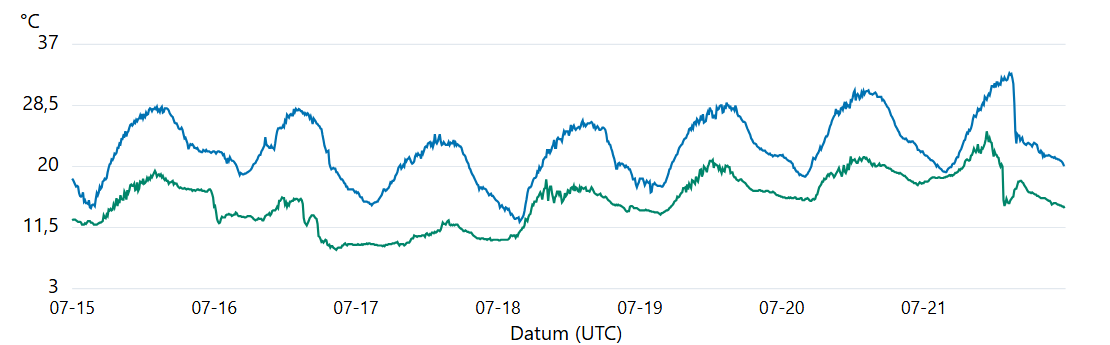
\includegraphics[width=\linewidth]{Abbildungen/mehrtagesansicht.png}
  \par\smallskip
  {\footnotesize\textcolor[HTML]{0072b2}{\rule{12pt}{2pt}} Wittenberg
  \quad\textcolor[HTML]{00856a}{\rule{12pt}{2pt}} Brocken\par}
  \caption{Echte Zeitraumansicht vom 15. bis 21. Juli 2024 mit
  Zehn-Minuten-Temperaturen von Wittenberg und Brocken. Beide Stationen
  besitzen 1008 von 1008 vorhandenen Werten. Die wiederkehrenden
  Tagesverläufe bleiben neben dem Stationsunterschied erkennbar.}
  \label{fig:range}
\end{figure}
Die Positionskodierung erlaubt, die Höhe zweier Temperaturen an derselben
Zeitposition unmittelbar zu vergleichen. Die Linie unterstützt das Lesen
zeitlicher Veränderungen; Stationen unterscheiden sich zusätzlich durch
Farbe und Beschriftung. Ihre Verbindung bedeutet keine Messung zwischen
zwei Rasterpunkten. Das Diagramm bleibt expressiv, indem es nur gültige
benachbarte Werte verbindet und die Auflösung ausdrücklich bezeichnet.
Eine vertikale Nullbasis ist für Temperaturverläufe nicht erforderlich;
die gemeinsame Achse und ihre Grenzen bleiben jedoch sichtbar.

Die Alternativen lösen unterschiedliche Teilaufgaben. Eine Tabelle
liefert genaue Einzelwerte und Rangfolgen; für die Frage, wann ein
Stationsabstand innerhalb der Woche wächst, müssten jedoch viele Zeilen
verglichen werden. Die Linien legen dafür beide Temperaturen an dieselbe
Zeitposition. Getrennte Panels reduzieren Verdeckung, verlangen bei
gleichen Skalen aber den Blickwechsel zwischen zwei vertikalen Positionen;
mit unterschiedlichen Skalen wären scheinbar gleiche Kurvenabstände
irreführend. Eine einzelne Differenzlinie zeigte den Abstand direkt,
verlöre jedoch die absoluten Temperaturen beider Orte. Deshalb kombiniert
der Entwurf überlagerte Linien für höchstens vier Stationen mit
Stationswahl und einer genauen Tabelle.

Horizon Graphs reduzieren den Platzbedarf durch Schichtung und Farbe.
Heer et al. untersuchen, wie Höhe und Schichtung die Leistung bei
Zeitreihenvergleichen beeinflussen \autocite{heer2009horizon}.
Das begründet die Prüfung von Darstellungsdichte und Aufgabe, belegt aber
keine Überlegenheit unseres Wetterdiagramms. Für den gleichzeitigen
Vergleich weniger absoluter Temperaturen vermeidet die gemeinsame
gewöhnliche Skala einen zusätzlichen Dekodierschritt. Verdeckung bleibt
eine Grenze; sie wird durch Eingrenzung vermindert und nicht als gelöst
ausgegeben.
\subsubsection{Visualisierung Zwei}
Die implementierten parallelen Koordinaten zeichnen eine Linie pro
vollständigem Stations-/Tagesprofil. Die vier vertikalen Achsen kodieren
Temperaturmittel, Feuchtigkeitsmittel, Windmittel und Niederschlagssumme.
Jede Achse besitzt ihre eigene Einheit. Die stationstypische Linienfarbe
wird aus dem Tagesdiagramm übernommen.

Die festen Skalen reichen von $-15$ bis 30\,°C, 0 bis 100\,\%,
0 bis 30\,m/s und 0 bis 60\,mm. Sie wurden anhand der zuvor geprüften
Jahresdaten gewählt; beim Filtern werden sie nicht verändert. Die
Browserprüfung bestätigte, dass alle dargestellten Profilwerte innerhalb
dieser Bereiche liegen. Diese Wertebereiche gelten für den gewählten
Projektumfang. Eine Erweiterung auf andere Jahre oder Stationen erfordert
eine erneute Skalenprüfung.

Von 1464 Stations-/Tagen besitzen 1442 alle vier erforderlichen
Tageskennzahlen. Die 22 übrigen Profile werden gezählt und nicht als
vollständige Linien gezeichnet. Ihre vorhandenen Einzelkennzahlen bleiben
in der Tagesübersicht zugänglich. Reguläre Linien besitzen eine geringe
Deckkraft; Linien des ausgewählten Tages werden stärker gezeichnet und
liegen über dem Kontext. Wertefilter blenden unpassende Profile ab.
Die Darstellungswahl erlaubt zusätzlich, nur passende Profile oder nur
passende Profile des ausgewählten Tages zu zeichnen. Sie verändert
weder die Filter noch die Trefferzahl; die Anzahl gezeichneter Profile
wird gesondert angezeigt.
Die große Zahl überlagerter Linien macht genaue Einzelvergleiche ohne
Auswahl schwierig; Filter und Tagesdetails unterstützen die Untersuchung.
Diese Gestaltungsfragen stehen im Zusammenhang mit den in der Literatur
behandelten Möglichkeiten und Grenzen paralleler Koordinaten
\autocite{heinrich2013parallel}.
\begin{figure}[htbp]
  \centering
  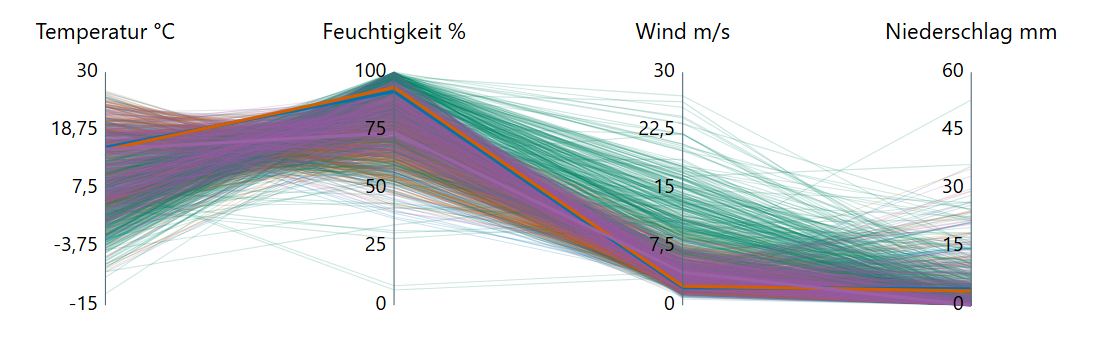
\includegraphics[width=\linewidth]{Abbildungen/parallele_koordinaten.png}
  \par\smallskip
  {\footnotesize Achsen von links nach rechts: Temperatur $-15$ bis 30\,°C;
  Feuchtigkeit 0 bis 100\,\%; Wind 0 bis 30\,m/s;
  Niederschlag 0 bis 60\,mm.\par}
  {\footnotesize
  \textcolor[HTML]{0072b2}{\rule{10pt}{2pt}} Wittenberg \quad
  \textcolor[HTML]{d55e00}{\rule{10pt}{2pt}} Leipzig/Halle \quad
  \textcolor[HTML]{00856a}{\rule{10pt}{2pt}} Brocken \quad
  \textcolor[HTML]{9a61a4}{\rule{10pt}{2pt}} Hamburg\par}
  \caption{Diagrammausschnitt der implementierten parallelen Koordinaten:
  1442 vollständige Wetterprofile, hervorgehobener Tag 19. Juni 2024.
  Für Brocken fehlen sieben Niederschlagsintervalle; dessen Profil wird
  deshalb nicht hervorgehoben. Einzelkennzahlen, Filter und Trefferzahl
  sind in der Anwendung zusätzlich zugänglich.}
  \label{fig:profiles}
\end{figure}
Die vier Achsen trennen quantitative Attribute mit unterschiedlichen
Einheiten; verbundene Positionen gehören zu einem Stations-/Tag.
Verbindungssegmente stellen weder zeitliche Übergänge noch eine
physikalische Zwischenmessgröße dar. Diese Bedeutung ist für die
Expressivität entscheidend. Temperatur und Feuchtigkeit stehen zuerst,
Wind und Niederschlag folgen als ergänzende Wettergrößen. Die Reihenfolge
ist für die gewählten Aufgaben fest und nicht als beste Anordnung für
sämtliche Korrelationen belegt.
Für die Frage nach Wind und Niederschlag liegen diese beiden Achsen
nebeneinander. Zwei Intervalle bilden ihre Schnittmenge, während
Temperatur und Feuchtigkeit den Kontext der verbleibenden Profile
sichtbar halten. So bleibt beim zusätzlichen Filter unmittelbar
erkennbar, ob dieselben Stations-/Tage beide Bedingungen erfüllen.

Der Forschungsüberblick behandelt Achsenreihenfolge, Interaktion und
Überlagerung als zentrale Gestaltungsfragen
\autocite[Abschnitte~5--6]{heinrich2013parallel}. Hier verringern geringe
Deckkraft und hervorgehobene Auswahl die visuelle Konkurrenz, beseitigen
aber die Überlagerung von 1442 Profilen nicht. Linienintensität erlaubt
deshalb keine verlässliche Häufigkeitsmessung. Die angezeigte Trefferzahl
und Detailtabelle ergänzen die grafische Übersicht. Eine sortierte Tabelle
wäre für exakte Werte und Rangfolgen direkter; eine Scatterplot-Matrix
unterstützte Paarbeziehungen, benötigte für vier Größen jedoch mehrere
Teilbilder. Parallele Koordinaten unterstützen hier besonders die
gleichzeitige Eingrenzung über vier Attribute. Der datenidentische
Wind-/Niederschlagsvergleich in Abbildung~\ref{fig:profile-comparison}
zeigt zugleich, wann zwei räumliche Achsen für eine engere Frage
leichter lesbar sind als vier verbundene Achsen.
\subsubsection{Visualisierung Drei}
Die implementierte Jahresübersicht ordnet Tage in neun Blöcken mit je
42 Positionen an. Das äußere Raster besitzt drei Spalten und drei Zeilen;
jedes innere Raster besitzt sieben Spalten und sechs Zeilen. Der eigene
Koordinatenerzeuger übernimmt die zeilenweise rekursive Traversierung aus
dem in der Veranstaltung bereitgestellten Verfahren. Die rekursive
Anordnung unterstützt hier die räumlich kompakte Darstellung einer
geordneten Folge; die Originalarbeit von Keim et al. ist eine methodische
Grundlage, kein Nachweis der Eignung dieser konkreten Wetterdarstellung
\autocite{keim1995recursive}.

366 Tage belegen 378 Positionen. Die zwölf übrigen Plätze bleiben leer und
besitzen eine gepunktete Umrandung. Innerhalb eines Blocks wird von links
nach rechts und zeilenweise nach unten gelesen, anschließend wird zum
nächsten Block gewechselt. Ein Block umfasst sechs Wochen und ist kein
Kalendermonat. Datumsbereiche beschriften die Blöcke; Zellen mit der Ziffer
1 kennzeichnen Monatsanfänge.

Eine gemeinsame, feste Farbskala kodiert das Temperaturtagesmittel in sieben
Bereichen: unter 0\,°C, 0 bis unter 5\,°C, 5 bis unter 10\,°C,
10 bis unter 15\,°C, 15 bis unter 20\,°C, 20 bis unter 25\,°C und
mindestens 25\,°C. Dunkle Farben stehen für niedrigere, hellere für höhere
Temperaturen. Diese Bereiche werden beim Filtern nicht neu berechnet.
Die Klasseneinteilung erlaubt eine grobe Jahresorientierung, verbirgt aber
Unterschiede innerhalb eines Bereichs. Der genaue Wert ist deshalb über
die Zelleninformation zugänglich.

Schraffuren unterscheiden fehlende vollständige Tagesmittel von einem
echten Nullwert. Noch ungeladene Monate und Abruffehler besitzen eigene
Darstellungen; sie werden nicht als Messwertlücken ausgegeben. Die
orangene Umrandung markiert den im Tagesdiagramm ausgewählten Tag über
alle sichtbaren Stationen hinweg.
\begin{figure}[htbp]
  \centering
  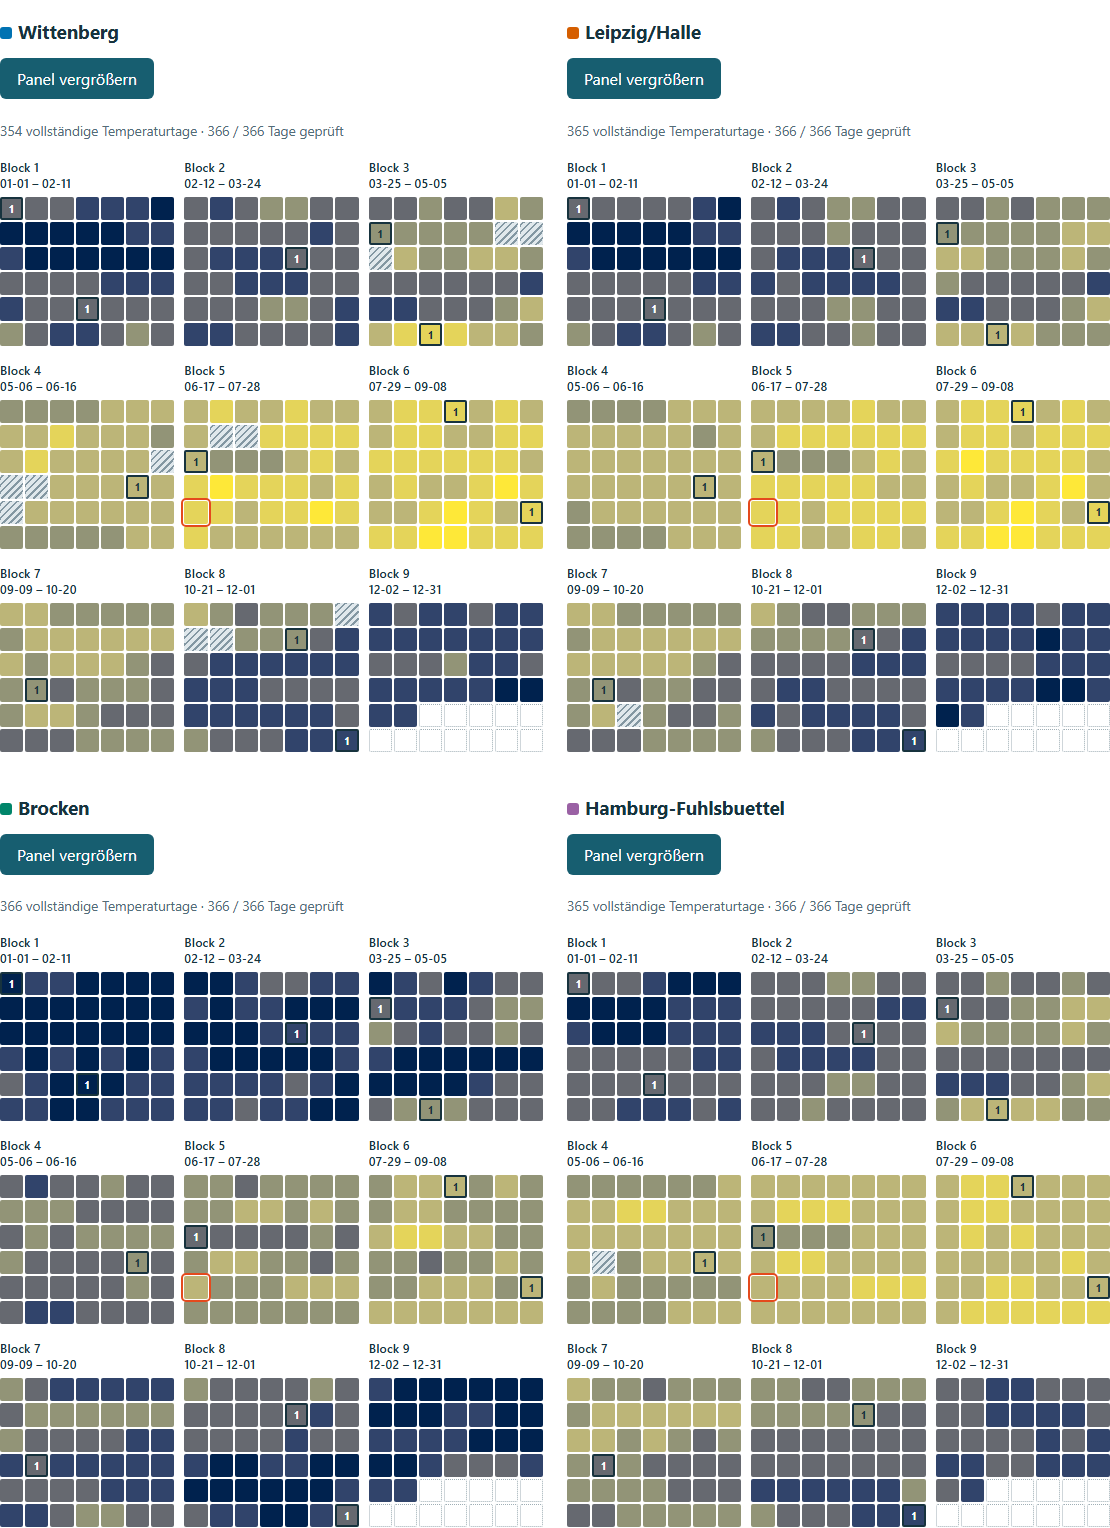
\includegraphics[width=\linewidth,height=0.72\textheight,keepaspectratio]{Abbildungen/jahresuebersicht.png}
  \par\smallskip
  {\footnotesize Temperaturmittel (°C):
  \textcolor[HTML]{00224e}{\rule{1em}{0.7em}}~$<0$\quad
  \textcolor[HTML]{31446b}{\rule{1em}{0.7em}}~$0$ bis $<5$\quad
  \textcolor[HTML]{666970}{\rule{1em}{0.7em}}~$5$ bis $<10$\quad
  \textcolor[HTML]{929477}{\rule{1em}{0.7em}}~$10$ bis $<15$\quad
  \textcolor[HTML]{bcb578}{\rule{1em}{0.7em}}~$15$ bis $<20$\quad
  \textcolor[HTML]{e4d45a}{\rule{1em}{0.7em}}~$20$ bis $<25$\quad
  \textcolor[HTML]{fee838}{\rule{1em}{0.7em}}~$\geq25$.\par}
  \caption{Tatsächliche Recursive-Pattern-Jahresübersicht nach dem geprüften
  Browserabruf am 3. Oktober 2026. Alle Panels verwenden dieselbe
  Tagesanordnung und dieselben festen Temperaturbereiche. Markiert ist der
  15. Juli; schraffierte Temperaturtage sind unvollständig, die zwölf
  gepunkteten Plätze am Ende gehören nicht zum Jahr.}
  \label{fig:year}
\end{figure}
Für die Orientierung im Jahr wird ein Tageswert auf eine Zelle abgebildet.
Identische Tagespositionen und eine gemeinsame Skala unterstützen den
Stationsvergleich. Die rekursive Gruppierung ordnet eine Zeitfolge
kompakt an \autocite{keim1995recursive}; die hier gewählten 42-Tage-Blöcke
übernehmen die zeilenweise Variante der Lehrmaterialien. Eine Zelle ist
eine Tagesaggregation und keine verlustfreie Darstellung aller Rohwerte.
Farben ermöglichen die Suche nach groben Bereichen; genaue quantitative
Vergleiche werden durch die Klassen begrenzt und benötigen Details.

Die Klassengrenzen bleiben beim Filtern unverändert, damit eine Farbe
ihre Bedeutung behält. Eine Kalender-Heatmap hätte vertrautere Monats-
und Wochenbezüge. Die rekursive Anordnung benötigt deshalb Blockbereiche,
Monatsanfänge und eine ausdrückliche Leserichtung. Eine Jahreslinie würde
genaue Wertabstände und Nulldurchgänge besser darstellen, bietet aber eine
andere räumliche Übersicht. Recursive Pattern wird hier für Orientierung
und Tageswahl eingesetzt; die Vorlesungstechnik allein begründet keinen
Wahrnehmungsvorteil gegenüber diesen Alternativen.
Identische Datumspositionen erleichtern den Vergleich mehrerer Panels.
Die zusätzliche Lesehilfe nummeriert die Blockfolge von 1 bis 9;
kräftigere Rahmen markieren Monatsanfänge. Diese Hilfen reduzieren
Orientierungsaufwand, ersetzen aber nicht die vertrauten Monatsbezüge
eines Kalenders. Den direkten Entwurfsvergleich für dieselbe
Vorzeichenfrage zeigt Abbildung~\ref{fig:calendar-comparison}.

Der Differenzmodus ersetzt die Stationspanels durch ein Panel für ein
geordnetes Stationspaar A und B. Jede Zelle kodiert das Temperaturmittel
von A minus B. Die feste divergierende Farbskala ist um null zentriert:
Blau bedeutet A kälter, Rot A wärmer und die neutrale Mitte eine Differenz
von null. Die Grenzen liegen bei $-10$, $-5$, $-2$, 0, 2, 5 und
10\,°C; die Legende benennt auch die offenen und geschlossenen Grenzen.
Eine vollständige Differenz erfordert dieselben 144 verwendbaren
Zeitpunkte und zwei vollständige Tagesmittel. Elm speichert deshalb
zusätzlich die Menge vorhandener Temperatur-Zeitplätze je Tag und bildet
ihre Schnittmenge. Bei vollständiger gemeinsamer Abdeckung ist die
Differenz der beiden Mittel gleich dem Mittel der paarweisen Differenzen.
Bei unvollständiger Abdeckung bleibt die Tagesdifferenz fehlend; Zahl und
längste Fehlstelle der gemeinsamen Zeitplätze bleiben ablesbar.
\begin{figure}[htbp]
  \centering
  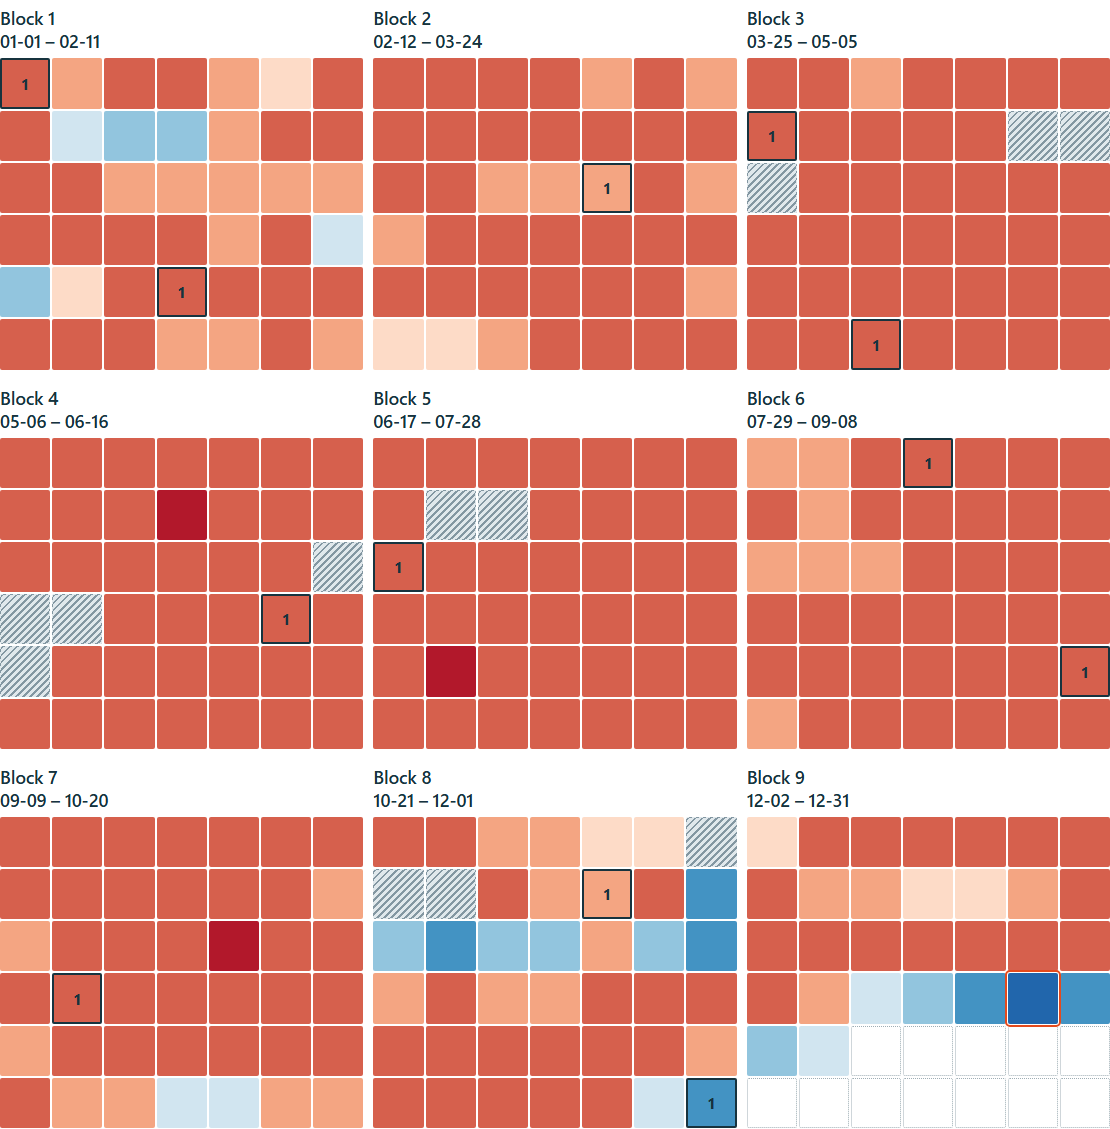
\includegraphics[width=\linewidth,height=0.68\textheight,keepaspectratio]{Abbildungen/jahresdetail.png}
  \par\smallskip
  {\footnotesize Differenz $\Delta =$ Wittenberg minus Brocken (°C):\par
  \begin{tabular}{lll}
  \textcolor[HTML]{2166ac}{\rule{1em}{0.7em}}~$\Delta\leq-10$ &
  \textcolor[HTML]{4393c3}{\rule{1em}{0.7em}}~$-10<\Delta\leq-5$ &
  \textcolor[HTML]{92c5de}{\rule{1em}{0.7em}}~$-5<\Delta\leq-2$\\
  \textcolor[HTML]{d1e5f0}{\rule{1em}{0.7em}}~$-2<\Delta<0$ &
  \textcolor[HTML]{888888}{\fbox{\textcolor[HTML]{f7f7f7}{\rule{0.8em}{0.5em}}}}~$\Delta=0$ &
  \textcolor[HTML]{fddbc7}{\rule{1em}{0.7em}}~$0<\Delta<2$\\
  \textcolor[HTML]{f4a582}{\rule{1em}{0.7em}}~$2\leq\Delta<5$ &
  \textcolor[HTML]{d6604d}{\rule{1em}{0.7em}}~$5\leq\Delta<10$ &
  \textcolor[HTML]{b2182b}{\rule{1em}{0.7em}}~$\Delta\geq10$
  \end{tabular}\par}
  \caption{Vergrößertes Jahrespanel des geprüften Differenzmodus für Wittenberg minus Brocken,
  ausgewählter 28. Dezember 2024. Dunkle Rahmen markieren Monatsanfänge,
  die orange Markierung bezeichnet den ausgewählten Tag.
  354 Tage besitzen vollständige gemeinsame Vergleichswerte;
  Schraffuren markieren die zwölf unvollständigen Tage. Die zwölf
  unbenutzten Rasterplätze am Ende bleiben gesondert gekennzeichnet.
  Negative und positive Unterschiede verwenden dieselbe feste Farbskala.}
  \label{fig:difference}
\end{figure}

\subsection{Interaktion}
Ein Stationswechsel aktualisiert Jahrespanels und Profile unmittelbar.
Tagesdetails und ein bereits übernommener Zeitraum werden nach
250\,ms ohne weitere Stationsänderung automatisch übernommen. Dabei bleibt der
geladene Detailtag erhalten; eine noch nicht übernommene Datumseingabe
wird nicht versehentlich geladen. Ein neues Datum wird weiterhin mit
der Schaltfläche bestätigt. Bei leerer Stationswahl werden Tages- und
Zeitraumdaten aus der Anzeige entfernt. Anfragegenerationen verhindern,
dass verspätete Antworten vorheriger Auswahlen zurückkehren.

Ein Klick oder eine Aktivierung per Eingabetaste
in der Jahresübersicht übernimmt den Zelltag und lädt die Tagesdetails.
Die übrigen aktiven Stationen bleiben für den Vergleich ausgewählt.
Auch ein Tag mit fehlendem Tagesmittel bleibt auswählbar, damit die
vorhandenen Rohwerte und deren Abdeckung überprüft werden können.
Die Auswahl wird umgekehrt auch beim Laden über das Datumsfeld in den
Jahrespanels markiert. Pfeiltasten bewegen ausschließlich den Fokus um
einen oder sieben Tage; erst die Aktivierung löst einen Tagesabruf aus.
Unter jeder Profilachse erlauben zwei Regler die Auswahl einer unteren und
oberen Wertgrenze. Aktive Intervalle werden durch logisches UND verbunden.
Nur vollständige Profile, die alle Intervalle erfüllen, gelten als passend.
Ihre Tageszellen bleiben in der Jahresübersicht hervorgehoben;
andere Zellen werden abgeblendet. Im Tagesdiagramm werden die
Temperaturreihen unpassender Stations-/Tage abgeblendet und bleiben als
Rohwertkontext erhalten. Linien verbinden weiterhin ausschließlich
zeitlich benachbarte vorhandene Messwerte, unabhängig von der Profilwahl.

Ein Klick auf eine Profillinie übernimmt deren Datum für die Tagesdetails.
Die Linien des gewählten Tages lassen sich auch per Tastatur aktivieren.
Zusätzlich bietet eine native Auswahl die aktuell passenden Profile an.
Die Suche grenzt diese Liste nach Stationsnamen und Datum ein; sowohl
ISO-Datum als auch Tag.Monat.Jahr sind möglich. Mehrere Suchwörter gelten
gemeinsam, unabhängig von Groß- und Kleinschreibung. Die Suche verändert
nur den Zugang zur Auswahl, nicht die Wetterfilter oder die Diagramme;
ihre separate Trefferzahl benennt diesen Unterschied. Eine leere Liste
wird deaktiviert. So bleibt ein bekanntes Datum ohne präzisen Linienklick
erreichbar. Die Rücksetztaste entfernt Profilintervalle und Suchtext und stellt
die Darstellung des Gesamtkontexts wieder her,
ohne Datum oder Stationswahl zu verändern.

Start- und Enddatumsfelder übernehmen einen zusammenhängenden Zeitraum.
Die Jahresübersicht bleibt vollständig sichtbar und markiert den
Zeitbereich. Parallele Koordinaten zeigen nur die Profile dieses Bereichs;
außerhalb liegende Tage werden nicht als unvollständige Profile gezählt.
Im Zeitraumdiagramm bleiben unpassende Profile als abgeblendeter
Temperaturkontext erhalten. Passende, nicht benachbarte Tage werden
nicht über dazwischenliegende Tage hinweg verbunden. Im Differenzpanel
müssen beide Stationsprofile die aktiven Werteintervalle erfüllen.

Die Aktivierung eines Tages außerhalb des gewählten Zeitraums hebt diesen
mit einem sichtbaren Hinweis auf. Ein Stationspaarwechsel setzt den
Zeitraum ebenfalls zurück. Die beiden Vergleichsstationen bleiben im
Differenzmodus ausgewählt. Das globale Zurücksetzen entfernt Zeitraum,
Profilintervalle und Differenzmodus und stellt alle vier Stationen sowie
den 15. Juli als Detaildatum wieder her. Geladene Jahresdaten bleiben dabei
erhalten; Abmeldung löscht dagegen die Sitzungscaches.
Einzelne Jahrespanels lassen sich auf die verfügbare Breite vergrößern;
auf schmalen Geräten bleibt das größere Raster innerhalb des Panels
horizontal verschiebbar. Positionen, Farben und Tagesauswahl ändern sich
dabei nicht (Abbildung~\ref{fig:difference}).
Die Verknüpfung folgt dem Zusammenspiel von Auswahl, Filterung, Navigation
und koordinierten Ansichten \autocite{heer2012interactive}. Der Jahresklick
wechselt vom Überblick zum zeitlichen Detail. Profilintervalle grenzen
mehrdimensionale Datensätze ein und behalten ihre zeitliche Lage im Jahr.
Die Zeitraumwahl reduziert Profile, erhält aber den Jahreskontext.
Damit muss das Datum eines auffälligen Profils nicht manuell in einer
anderen Ansicht gesucht werden. Die drei tatsächlichen Anwendungsabläufe
belegen die Weitergabe der Auswahl. Ob dies für die Zielgruppe schneller
oder verständlicher als unabhängige Ansichten ist, bleibt zu evaluieren.
Der automatische Stationswechsel vermeidet einen zusätzlichen
Übernahmeschritt. Eine kurze Wartezeit bündelt schnelle Änderungen;
validierte Stations-/Tagesdaten werden innerhalb der Sitzung wiederverwendet.
Die Schaltflächen zum Laden des Detailtags und zum erneuten Zeitraumabruf
umgehen diese Rohwertcaches ausdrücklich. Generationen schützen den Zustand,
brechen aber bereits laufende Anfragen nicht physisch ab. Geladene Jahres- und Profildaten werden
ohne erneuten Abruf gefiltert. Ein neuer Stationspaarvergleich setzt
den Zeitraum zurück, damit alte Zeitraumdaten nicht einem anderen Paar
zugeordnet werden.

Eine rechteckige Auswahl im Jahresraster wurde nicht umgesetzt, weil sie
bei den Blockwechseln keinen eindeutigen zusammenhängenden Zeitraum
repräsentiert. Start-/Enddatum beschreiben diesen stattdessen ausdrücklich.
Achsenumordnung ist für die feste Frage nach mehreren Werteintervallen
nicht erforderlich; die Anwendung untersucht keine beliebigen
Korrelationshypothesen. Deshalb bleibt die Reihenfolge beschriftet und
stabil. Grafisches Zoomen wurde zugunsten einer ausdrücklich gewählten
Zeitspanne und benannter Auflösung weggelassen. Auch die Profilwahl hat
eine Grenze: Per Tastatur sind die Linien des bereits ausgewählten Tages
aktivierbar; die native Profilauswahl ergänzt deshalb einen Zugang zu allen
aktuell passenden Profilen. Beliebige Tage können über Jahreszellen oder das
Datumsfeld gewählt werden. Damit wird keine vollständige Barrierefreiheit
behauptet.

\section{Implementierung}
\begin{figure}[htbp]
  \centering
  \begingroup
\setlength{\unitlength}{1pt}
\begin{picture}(420,124)
\put(0,84){\framebox(120,36){\shortstack{\small Main: Auswahl / Msg\\\small Zustandsübergang}}}
\put(150,84){\framebox(120,36){\shortstack{\small Api / Profiles\\\small HTTP-Kommando}}}
\put(300,84){\framebox(120,36){\shortstack{\small Uni-Schnittstelle\\\small JSON-Antwort}}}
\put(120,102){\vector(1,0){30}}
\put(270,102){\vector(1,0){30}}
\put(360,84){\vector(0,-1){36}}
\put(300,12){\framebox(120,36){\shortstack{\small Weather / Profiles\\\small Decoder / Validierung}}}
\put(150,12){\framebox(120,36){\shortstack{\small Year / Profiles\\\small Tagesaggregation}}}
\put(0,12){\framebox(120,36){\shortstack{\small Main.Model / Views\\\small Kennzahlen / Anzeige}}}
\put(300,30){\vector(-1,0){30}}
\put(150,30){\vector(-1,0){30}}
\end{picture}
\endgroup

  \caption{Datenfluss eines erfolgreichen Abrufs. Nutzeraktionen erzeugen
  Elm-Nachrichten und HTTP-Kommandos; gültige Antworten werden aggregiert
  und dargestellt. Fehlerantworten gehen in einen sichtbaren Fehlerzustand.
  Generationen verhindern die Übernahme veralteter Antworten.
  Der lokale Server liefert nur statische Dateien.}
  \label{fig:architecture}
\end{figure}
Die Anwendung verwendet Elm 0.19.1. Abbildung~\ref{fig:architecture}
ordnet die Module nach dem Datenfluss: \texttt{Main} verwaltet Auswahl,
Nachrichten und Zustandsübergänge; \texttt{Api} kapselt Anmeldung und
Messdatenanfragen. \texttt{Weather} stellt Messwerttyp, Decoder,
UTC-Grenzen und Validierung bereit. \texttt{Year} und \texttt{Profiles}
bilden Tageskennzahlen; letzteres verwaltet zusätzlich die Wind-/Regenabrufe.

Die Darstellung ist getrennt: \texttt{Recursive} erzeugt Positionen,
\texttt{YearView} zeichnet Jahrespanels und \texttt{ProfileView}
Profile, Filter und Auswahl. \texttt{Difference} berechnet gemeinsame
Abdeckung und Differenzen. \texttt{Range} verwaltet Zeiträume und begrenzte
Rohwertabrufe, \texttt{RangeView} zeichnet die Reihen.
\texttt{DailyCache} begrenzt die wiederverwendeten validierten
Stations-/Tagesreihen. Die folgenden
Model-Auszüge erklären den gemeinsamen Interaktionszustand.

Anfragen tragen eine fortlaufende Generation. Späte Antworten eines älteren
Abrufs werden verworfen, sodass sie einen neueren Zustand nicht
überschreiben. Passwort und Sitzungstoken werden nicht in Local Storage oder
Session Storage gespeichert. Der lokale Node-Server liefert ausschließlich
die statischen Anwendungsdateien; die HTTP-Anfragen sendet Elm direkt an den
Uni-Server.

Der Jahresabruf umfasst 48 Stationsmonate. Eine Warteschlange lässt höchstens
zwei Jahresanfragen gleichzeitig zu. Anfragen verlangen maximal 5000 Zeilen
pro Seite. Ist das Monatsraster noch nicht vollständig, wird mit dem
Offset der tatsächlich erhaltenen Zeilen weitergeladen, bis eine leere
Abschlussseite eintrifft oder alle erwarteten Zeitpunkte vorliegen.
Validierung erfolgt vor Übernahme des Monats. Ein Sicherheitslimit von zwölf
Seiten verhindert unbegrenzte Anfragefolgen; eine Überschreitung wird als
Abruffehler angezeigt. Nach der Aggregation werden die Monatsrohwerte
verworfen, erfolgreiche Tagesaggregate bleiben für die Sitzung erhalten.
Fehlgeschlagene Monate lassen sich erneut laden, ohne erfolgreiche Monate
abermals abzurufen. Tages- und Jahresanfragen verwenden getrennte
Generationen, damit ein Tageswechsel keinen Jahresabruf ungültig macht.
Nach dem Temperatur-Jahresabruf werden 96 weitere Feld-/Stationsmonate
für Wind und Niederschlag geladen, wiederum mit höchstens zwei
gleichzeitigen Anfragen. Dieser zweite Abruf kann erst nach Abschluss der
ersten Jahreswarteschlange gestartet werden. Erfolgreiche Intervallmonate
bleiben bei gezielter Wiederholung fehlgeschlagener Monate erhalten.
Abmeldung löscht Kennzahlen und Filter; alte Antworten dürfen den neuen
Sitzungszustand nicht überschreiben.

Der Datenfluss beginnt mit einer Auswahl in \texttt{Main}; ein
HTTP-Kommando aus \texttt{Api} liefert eine Nachricht mit
\texttt{Result}. Validierte Messwerte werden zu Tageskennzahlen
aggregiert und an die View-Module übergeben. Fehler bleiben als eigener
Zustand sichtbar. Der folgende Auszug enthält ausschließlich die für
Auswahl und Antworten wesentlichen Felder des tatsächlichen Models;
Anmeldung, Warteschlangen und weitere Felder sind ausgelassen.
\begin{verbatim}
type alias Model =
    { selected : Set Int
    , dateInput : String
    , requestDay : Maybe String
    , yearDays : Dict Int (Dict String Year.Daily)
    , profiles : Profiles.Model
    , filters : Dict Int ( Float, Float )
    , range : Range.Model
    , generation : Int
    -- Weitere Felder sind hier ausgelassen.
    }
\end{verbatim}
Zwei relevante Konstruktoren aus \texttt{Msg} sind
\texttt{ChooseYearDay} und \texttt{GotMeasurements}.
Die erste Nachricht trägt Stations-ID und Datum, die zweite zusätzlich
die Anfragegeneration und das Ergebnis als
\texttt{Result Http.Error (List Measurement)}.
Ein Jahresklick löst \texttt{ChooseYearDay} aus: Das Datum und der Fokus
werden übernommen, die Station wird in die Auswahl eingefügt und
\texttt{Load} startet den Tagesabruf. Dieser setzt den geladenen
Tageskontext und erhöht die Anfragegeneration. Erst eine passende
\texttt{GotMeasurements}-Antwort aktualisiert das Ergebnis.
\texttt{ProfileFilter} verändert dagegen die Intervallgrenzen ohne neuen
Datenabruf; die Views berechnen daraus gemeinsame Hervorhebungen.

Die technischen Prüfungen vergleichen die Jahreskennzahlen mit getrennt
erzeugten CSV-Nachweisen: 2928 Temperatur-/Feuchtigkeitsauswertungen,
5768 Kennzahlen der 1442 Profile und 2196 Paar-/Tagesvergleiche.
Kontrollierte Antworten prüfen insbesondere Pagination, Fehlwerte,
Mitternacht, Schaltjahr, Jahresende und verspätete Antworten.
Der echte HTTP-Zugriff deckte einen unzulässigen CORS-Header
\texttt{Prefer} auf; dessen Entfernung behob den Browserabruf.
Die Prüfskripte liegen unter \texttt{app/scripts}; die zugehörigen
CSV-Nachweise liegen unter \texttt{Datenpruefung} und \texttt{Entwurf}.

Die Zeitraumwarteschlange erlaubt höchstens zwei gleichzeitige
Zeitraumanfragen. Eine Woche mit vier Stationen umfasst 4032
Temperatur-Zeitplätze. Die beiden getrennten Rohwertcaches für Detailtage
und Zeiträume speichern jeweils höchstens 28 zuletzt abgelegte
Stations-/Tagesreihen: zusammen höchstens 8064 Zeitplätze mit Temperatur
und Feuchtigkeit. Das ist eine Grenze der Cache-Einträge, keine Messung
des gesamten Speicherverbrauchs; angezeigte Ergebnisse und laufende
Antwortpuffer kommen hinzu. Fehlgeschlagene oder ungültige Antworten
werden nicht gecacht. Abmeldung und neue Anmeldung leeren beide Caches.
Ein ausdrücklich erneuter Tages- oder Zeitraumabruf umgeht den jeweiligen
Cache. Ohne diesen Schritt bleiben erfolgreich geladene Daten bis zur
Verdrängung wiederverwendbar; Änderungen am Server werden dann nicht
automatisch erkannt.

Längere Zeiträume verwenden Tagesaggregate des Jahrescaches. Die
gleichzeitig aktualisierten Einzeltagesdetails besitzen einen getrennten
Abruf; die Grenze von zwei gilt daher nicht für alle HTTP-Anfragen
zusammen. Stationsänderungen erhöhen sofort die Antwortgeneration und
eine Revisionsnummer. Erst die nach 250\,ms noch aktuelle Revision startet
die nächste Übernahme. Die Verzögerung ist eine Entwurfsentscheidung,
kein gemessener optimaler Wert. Alte Antworten werden verworfen; bereits
laufende HTTP-Anfragen werden nicht physisch abgebrochen.

Die Vergleichsprüfung bestätigt gemeinsame Temperaturabdeckung,
Vorzeichen und die Sieben-/Acht-Tage-Grenze. Der erweiterte Profilfall
prüft außerdem die gemeinsame Wind-/Niederschlagsauswahl, ein leeres
Ergebnis und die Rücknahme nur einer Bedingung. Diese Nachweise belegen
Berechnungen und Zustandsübergänge; sie ersetzen keine Bewertung der
Verständlichkeit durch die Zielgruppe.

Ein zentraler Rohdatentyp in \texttt{Weather.elm} lautet:
\begin{verbatim}
type alias Measurement =
    { stationId : Int
    , timestamp : String
    , temperature : Maybe Float
    , humidity : Maybe Float
    , quality : Int
    }
\end{verbatim}
\texttt{Maybe Float} trennt fehlende Werte von vorhandenen Nullwerten.
Decoderfehler und HTTP-Fehler werden dagegen mit \texttt{Result}
behandelt. Das Hauptmodel speichert Stationsmengen als \texttt{Set Int}
und Jahreskennzahlen als verschachtelte \texttt{Dict}-Struktur mit
Stations-ID und Datum. Ein \texttt{Year.Daily} enthält getrennte
Temperatur-/Feuchtigkeitsabdeckung, optionale Mittel, die längste
Temperaturlücke und die Menge vorhandener Temperatur-Zeitplätze.
Diese Menge ermöglicht die exakte gemeinsame Abdeckung eines
Stationspaars ohne die Speicherung sämtlicher Jahresrohwerte.
Wind-/Niederschlagskennzahlen liegen in einer \texttt{Dict}-Struktur mit
Stations-ID, Messart und Datum. Jedes \texttt{Profiles.Stat} enthält
Anzahl, optionalen Wert, Lücke und Qualitätsabweichung. Profilfilter
speichern je Achse untere und obere Grenze; mehrere Intervalle gelten
gemeinsam. Der Suchtext \texttt{profileQuery} beschränkt ausschließlich
die native Auswahlliste. Der Zustand der Zeitraumansicht enthält Datumsgrenzen,
Stationsauswahl, Ergebnisse, Warteschlange und eigene Abrufgeneration.

Der Aufwand lässt sich nach einfachen Grundlagen und schwierigen
Erweiterungen unterscheiden. Das zeilenweise rekursive Grundverfahren
war durch das bereitgestellte \texttt{createPixelMap}-Beispiel bereits
konkret vorgegeben. Der eigene kurze Koordinatenerzeuger übernimmt dessen
Prinzip mit außen nach innen angeordneten Ebenen; der Abgleich aller
378 Positionen dokumentiert diese Beziehung. Die Quellenbezeichnung
steht im Modul \texttt{Recursive} und im Entwurfsnachweis.
SVG-Achsen, Linien und Formularereignisse waren überschaubare
Grundbausteine. Vollständige Übungsmodule wurden dabei nicht unverändert übernommen.

Aufwändiger waren das Zusammenführen der nominalen Wind-/Regenintervalle,
die Feldabdeckung, gemeinsame Temperaturzeitplätze und der Umgang mit
späten HTTP-Antworten. Diese Teile benötigten separate Zustände und
gezielte Fehlerprüfungen. Dabei wurden unter anderem ein unzulässiger CORS-Header entfernt und
ein Test an die gerundeten Anzeigewerte angepasst.
Eine belastbare Stundenaufzeichnung liegt nicht vor. Der technische
Entwurf und Code wurden überwiegend durch den Assistenten erstellt;
eigene Beiträge werden im KI-Abschnitt getrennt dokumentiert.

Die Datenhaltung wird durch begrenzte Monatsseiten, verworfene Monatsrohwerte,
höchstens sieben dargestellte Rohwerttage pro Zeitraum und die beschriebenen
Rohwertcaches begrenzt. Jahresaggregate und Zeitplatzmengen bleiben für die Sitzung verfügbar.
Die Jahresübersicht besitzt vier gleich angeordnete Raster; die
Profilansicht kann bis zu 1442 Linien enthalten. Technische Prüfungen
bestätigen Funktion und mobile Breite, ersetzen aber keine Messung von
Ladezeit, Bildrate oder Speicherverbrauch. Die Anwendung ist auf vier
Stationen und 2024 festgelegt. Serververfügbarkeit, Tokenlaufzeit und
CORS bleiben externe Abhängigkeiten. Eine Erweiterung des Datenumfangs
erfordert neue Prüfungen von Skalen, Messabdeckung und Darstellungsdichte.

Die Datei \texttt{START.txt} beschreibt Installation, Programmstart und
Berichtserzeugung. Quellcode und LaTeX-Dateien liegen im lokalen
Git-Repository. Der Link steht im Anhang.

\subsection*{KI-Nutzung und Überprüfung}
Für die Entwicklung und die Ausarbeitung des Berichts wurde Codex als
KI-Assistent eingesetzt. Zunächst wurden im Dialog die Fragen festgelegt, die die Anwendung
beantworten soll, und passende Visualisierungstechniken ausgewählt. Ich entschied mich für Wetterdaten
und übernahm die besprochenen Vorschläge für Zeitreihen, parallele
Koordinaten und Recursive Pattern. Daraus wurden die erforderlichen
Datenstrukturen, Aggregationen und Verknüpfungen der Ansichten abgeleitet.

Als Kontext erhielt der Assistent die Veranstaltungsanforderungen,
Informationen zu den vorhandenen Daten und ihrer Bereitstellung,
Übungsbeispiele sowie die in der Vorlesung verlinkten Erläuterungen zu
den verwendeten Techniken. Das bereitgestellte rekursive Verfahren diente
beispielsweise als Grundlage für die Tagesanordnung. Die Kolleginnenarbeit
wurde ergänzend als Anschauungsmaterial betrachtet; maßgeblich blieben
die aktuellen Veranstaltungsanforderungen.

Auf dieser Grundlage erstellte Codex das erste Elm-Grundgerüst und
wesentliche Teile der weiteren Implementierung, der Prüfskripte sowie
der Berichtstexte. Die Ergebnisse wurden anschließend schrittweise
durchgesehen und überarbeitet. Ich bewertete die dargestellten Ergebnisse,
traf Auswahlentscheidungen und veranlasste Änderungen, wenn Darstellung
oder Bedienung nicht den beabsichtigten Aufgaben entsprachen. Kleinere
Layoutkorrekturen nahm ich auch direkt vor, etwa an den Abmessungen von
Boxen und der Positionierung von Beschriftungen. Diese Eingriffe wurden
nicht einzeln nach Datei und Zeitpunkt protokolliert. Größere Änderungen
wurden im weiteren Dialog durch den Assistenten umgesetzt.

Die technische Kontrolle umfasste den Elm-Compiler, automatisierte
Browserprüfungen mit echten und kontrollierten HTTP-Antworten sowie
Abgleiche mit getrennt erzeugten CSV-Auswertungen. Codex führte diese automatisierten Prüfungen aus.
Ich sah mir die Anwendung zusätzlich selbst an. Konkrete Korrekturen betrafen unter anderem einen
unzulässigen CORS-Header, Fehlstellen in Zeitreihen und die Behandlung
verspäteter Antworten nach Auswahländerungen.

Codex erleichterte vor allem die Umsetzung und die wiederholten Tests.
Die Ergebnisse mussten dennoch geprüft werden: Auch kompilierender Code
kann Tage falsch zuordnen oder eine schwer verständliche Bedienung ergeben.
Meine Beiträge waren die Themen- und Variantenwahl, die Durchsicht,
Entscheidungen über Änderungen und kleinere Layoutanpassungen.
Große Teile des Codes und des Berichts stammen von Codex. Der \hyperref[app:ai-workflow]{Anhang zum KI-Vorgehen} fasst die
Kontextgrundlage und die Überarbeitungsschritte zusammen.

\section{Anwendungsfälle}
Die folgenden drei Abläufe untersuchen konkrete Fragen der Zielgruppe mit
den tatsächlichen Stationsdaten von 2024. Sie wurden am 4. Oktober 2026
automatisiert im Browser mit echten HTTP-Abrufen durchgeführt und gegen
die unabhängigen Jahresauswertungen geprüft. Die Abbildungen zeigen diese Anwendungsläufe.
Die Prüfung zeigt, ob sich die drei Aufgaben mit der Anwendung bearbeiten
lassen. Wie gut andere Personen damit zurechtkommen, wurde nicht in einer
Nutzerstudie untersucht; auch Bearbeitungszeiten wurden nicht gemessen.

\subsection{Anwendung Visualisierung Eins}
Die Frage lautet: Wie unterscheiden sich die Temperaturen von Wittenberg
und Brocken im Juli 2024, und was zeigt eine genauere Betrachtung der
Woche vom 15. bis 21. Juli? Das Stationspaar wird ausgewählt und der
Zeitraum auf den 1. bis 31. Juli gesetzt. Die Ansicht verwendet
beschriftete Tagesmittel; beide Reihen enthalten 31 vollständige Tage.
Anschließend wird der Zeitraum auf den 15. bis 21. Juli eingegrenzt.
Die Darstellung wechselt zu Zehn-Minuten-Werten mit je 1008 vorhandenen
Werten, wie Abbildung~\ref{fig:range} zeigt.

In der Wochenansicht sind wiederkehrende Tagesverläufe und eine gemeinsame
Abkühlung zum 17. Juli erkennbar. In beiden Reihen besitzt der 17. Juli das
niedrigste Tagesmittel der Woche: Wittenberg 19,35\,°C und Brocken
10,13\,°C. Die Tagesmittel Wittenbergs sind an allen sieben Tagen höher.
Die Differenz reicht von 6,03\,°C am 18. Juli bis 10,04\,°C am 16. Juli.
Am 15. Juli beträgt sie 6,88\,°C. Alle Differenzen wurden vor der Rundung
aus vollständigen, zeitlich vergleichbaren Reihen berechnet.
\begin{figure}[htbp]
  \centering
  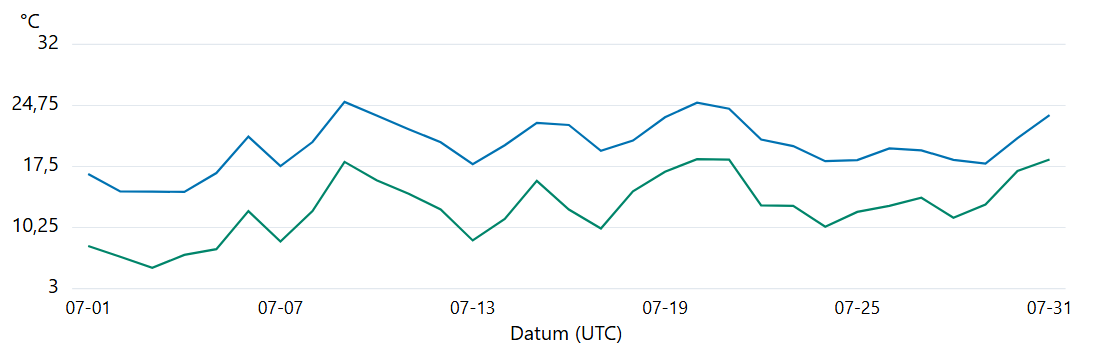
\includegraphics[width=\linewidth,height=0.36\textheight,keepaspectratio]{Abbildungen/anwendungsfall_monat.png}
  \par\smallskip
  {\footnotesize\textcolor[HTML]{0072b2}{\rule{12pt}{2pt}} Wittenberg
  \quad\textcolor[HTML]{00856a}{\rule{12pt}{2pt}} Brocken\par}
  \caption{Juli 2024 als vollständiger Tagesmittelvergleich zwischen
  Wittenberg und Brocken. Die beschriftete Auflösung unterscheidet sich
  ausdrücklich vom Wochenvergleich in Abbildung~\ref{fig:range}.}
  \label{fig:case-month}
\end{figure}

Der Nutzen für Wetterinteressierte besteht hier darin, vom Monatsüberblick
eine gemeinsame Veränderung zur genaueren Wochenprüfung auszuwählen.
An derselben horizontalen Position lassen sich beide Temperaturen
vergleichen. Bei getrennten Linienpanels muss diese Position zwischen
zwei Panels übertragen werden; eine Tabelle verlangt für den Wochenbefund
den Vergleich von sieben Zeilen. Eine sortierte Tabelle wäre dagegen
für die genaue Rangfolge der Tagesmittel direkter. Die gemeinsame Skala
und zwei unterscheidbare Reihen begründen hier die überlagerte Linie.
Diese Leseoperationen sind keine gemessenen Bearbeitungszeiten.

Tagesmittel verdecken die Veränderungen innerhalb eines Tages; die
Wochenansicht ergänzt deshalb die zeitlichen Details. Höhere Tagesmittel
beweisen nicht, dass eine Station zu jedem Zeitpunkt wärmer war.
Das Ergebnis gilt für diesen Zeitraum und diese Stationen und belegt
weder eine meteorologische Ursache noch einen langfristigen Klimatrend.

\subsection{Anwendung Visualisierung Zwei}
Die Frage lautet: Gibt es vollständige Tagesprofile mit einem Windmittel
von mindestens 20\,m/s und zugleich 0\,mm gemessenem Niederschlag?
Sie untersucht eine Schnittmenge zweier Wetterbedingungen statt einer
Rangliste. Für die Zielgruppe ist damit nachvollziehbar, welche
Tageskontexte eine ausgewählte Windbedingung begleiten. Temperatur und
Feuchtigkeit liefern zusätzlich den Kontext; Tageskennzahlen belegen
keine Gleichzeitigkeit innerhalb des Tages.

Nach globalem Zurücksetzen werden alle vier Stationen im gesamten Jahr
betrachtet. Die Winduntergrenze wird auf 20\,m/s gesetzt, alle anderen
Achsen bleiben uneingeschränkt. Es verbleiben 16 vollständige Profile,
sämtlich Brocken. Deren Linien verbinden hohe Windmittel mit positiven
Niederschlagssummen. Die unabhängig geprüften Summen reichen von
0,75 bis 24,41\,mm.

Anschließend wird die Niederschlagsobergrenze auf 0\,mm gesetzt. Da die
Untergrenze ebenfalls 0 beträgt, fordert der Filter genau den vorhandenen
Nullwert. Es bleiben keine passenden Profile und keine hervorgehobenen
Stations-/Tage im Jahresraster (Abbildung~\ref{fig:case-drywind}).
Die Anzeige benennt das leere Ergebnis; es ist kein Abruffehler.
Die Rücknahme nur der Niederschlagsbedingung auf 60\,mm stellt die
16 Windprofile wieder her. So ist die Wirkung der zweiten Bedingung
nachvollziehbar, ohne die erste Auswahl zu verlieren.
\begin{figure}[htbp]
  \centering
  {\small (a) Nur Windmittel $\geq20$\,m/s: 16 Treffer\par}
  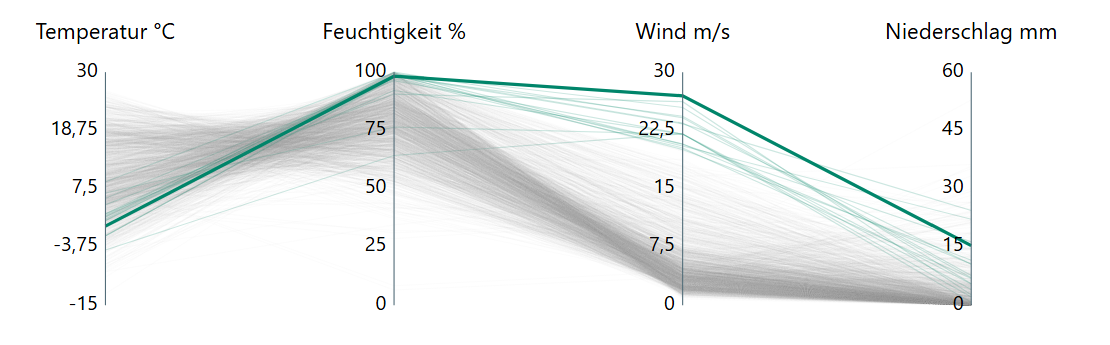
\includegraphics[width=\linewidth]{Abbildungen/anwendungsfall_wind.png}
  {\small (b) Zusätzlich Niederschlag $=0$\,mm: 0 Treffer\par}
  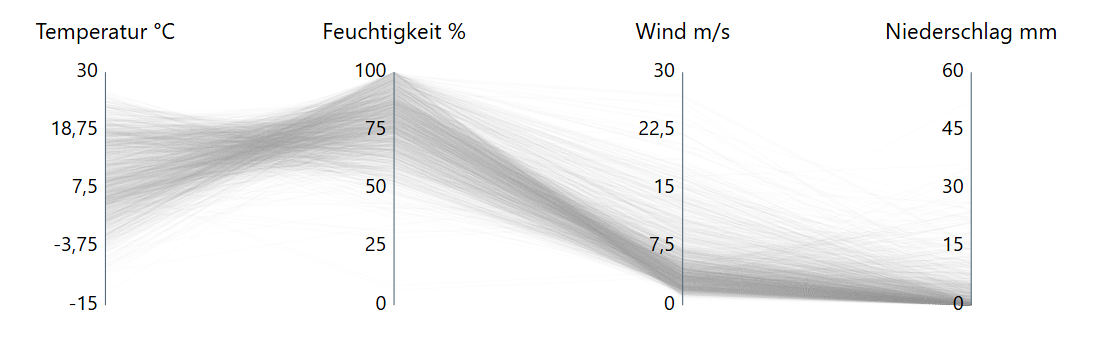
\includegraphics[width=\linewidth]{Abbildungen/anwendungsfall_wind_ohne_regen.png}
  \par\smallskip
  {\footnotesize Aktive Bedingungen: Wind $\geq20$\,m/s UND
  Niederschlag $=0$\,mm. Treffer: 0 von 1442 vollständigen Profilen.\par}
  \caption{Dieselben Achsenskalierungen vor und nach dem zweiten Filter.
  Die 16 passenden Windprofile besitzen positive Niederschlagssummen;
  die zusätzliche Bedingung entfernt sämtliche Treffer. Abgeblendete
  Profile bleiben in beiden Diagrammausschnitten als Kontext sichtbar.}
  \label{fig:case-drywind}
\end{figure}

Für ein konkretes Vergleichsprofil wird nach Rücknahme der
Niederschlagsbedingung der 22. Januar über die Profilauswahl geöffnet.
Brocken besitzt 0,28\,°C Temperaturmittel, 98,28\,\% Feuchtigkeitsmittel,
26,95\,m/s Windmittel und 15,35\,mm Niederschlagssumme.
Jede Kennzahl beruht auf 144 vorhandenen Werten. Die übrigen Stationen
bleiben im Detailvergleich erhalten (Tabelle~\ref{tab:windcase}).
Das größte verwendbare Windmittel ist ein zusätzlicher rechnerischer
Befund, kein Hauptargument für die Wahl paralleler Koordinaten.
\begin{table}[htbp]
  \centering
  \small
  \begin{tabular}{lrrrr}
    Station & Temperatur & Feuchtigkeit & Wind & Niederschlag \\
    & (°C) & (\%) & (m/s) & (mm) \\
    \hline
    Wittenberg & 6,43 & 77,74 & 5,22 & 1,77 \\
    Leipzig/Halle & 6,62 & 76,33 & 8,77 & 0,11 \\
    Brocken & 0,28 & 98,28 & 26,95 & 15,35 \\
    Hamburg-Fuhlsbuettel & 8,31 & 79,76 & 8,36 & 5,95 \\
  \end{tabular}
  \caption{Vollständige Stationsprofile vom 22. Januar 2024 (UTC).
  Temperatur, Feuchtigkeit und Wind sind Tagesmittel;
  Niederschlag ist eine Tagessumme.}
  \label{tab:windcase}
\end{table}

Eine sortierte Tabelle liefert exakte Werte und Maxima; die gemeinsame
Filterung muss auch dort dieselben Stations-/Tage betreffen. Die
datenidentische Projektion in Abbildung~\ref{fig:profile-comparison}
macht die engere Zweigrößenfrage räumlich direkt lesbar: Alle 16 grünen
Punkte liegen oberhalb beziehungsweise auf der Windgrenze und rechts
von 0\,mm. Ihre Niederschlagssummen reichen von 0,75 bis 24,41\,mm.
Für genau diese Frage ist das Streudiagramm eine gut begründete
Alternative; die zusätzliche 0-mm-Bedingung schneidet keinen grünen Punkt.
Es zeigt Temperatur und Feuchtigkeit jedoch nicht. Die parallelen
Koordinaten behalten diese Größen am selben Profil und erlauben weitere
Intervalle ohne Ansichtswechsel. Ihr Vorteil betrifft den erweiterten
Aufgabenumfang, während die Projektion weniger Achsenwechsel erfordert.
Die neue Wahl zwischen Gesamtkontext, passenden Profilen und ausgewähltem
Tag reduziert bei Bedarf die Linienmenge; die Trefferzahl bleibt dabei
unverändert. Ein Zeitvorteil wurde für keine Variante gemessen.
\begin{figure}[htbp]
  \centering
  \resizebox{\linewidth}{!}{% Geprüfte Projektion von 1442 vollständigen Profilen; 16 Windtreffer.
\begingroup\setlength{\unitlength}{1pt}
\begin{picture}(420,225)
\put(50,35){\rule{310pt}{0.5pt}}
\put(50,35){\rule{0.5pt}{160pt}}
\put(50,142){\color[HTML]{00856a}\rule{310pt}{0.5pt}}
\put(365,138){\scriptsize 20 m/s}
\put(50,32){\rule{0.4pt}{3pt}}
\put(40,19){\makebox(20,8){\scriptsize 0}}
\put(127.5,32){\rule{0.4pt}{3pt}}
\put(117.5,19){\makebox(20,8){\scriptsize 15}}
\put(205,32){\rule{0.4pt}{3pt}}
\put(195,19){\makebox(20,8){\scriptsize 30}}
\put(282.5,32){\rule{0.4pt}{3pt}}
\put(272.5,19){\makebox(20,8){\scriptsize 45}}
\put(360,32){\rule{0.4pt}{3pt}}
\put(350,19){\makebox(20,8){\scriptsize 60}}
\put(47,35){\rule{3pt}{0.4pt}}
\put(23,31){\makebox(20,8)[r]{\scriptsize 0}}
\put(47,88.33333333333333){\rule{3pt}{0.4pt}}
\put(23,84.33333333333333){\makebox(20,8)[r]{\scriptsize 10}}
\put(47,141.66666666666666){\rule{3pt}{0.4pt}}
\put(23,137.66666666666666){\makebox(20,8)[r]{\scriptsize 20}}
\put(47,195){\rule{3pt}{0.4pt}}
\put(23,191){\makebox(20,8)[r]{\scriptsize 30}}
\put(63.712,125.674){\color[HTML]{89959e}\rule{1.2pt}{1.2pt}}
\put(177.430,129.948){\color[HTML]{89959e}\rule{1.2pt}{1.2pt}}
\put(88.150,116.048){\color[HTML]{89959e}\rule{1.2pt}{1.2pt}}
\put(69.343,100.048){\color[HTML]{89959e}\rule{1.2pt}{1.2pt}}
\put(54.412,59.189){\color[HTML]{89959e}\rule{1.2pt}{1.2pt}}
\put(56.633,102.733){\color[HTML]{89959e}\rule{1.2pt}{1.2pt}}
\put(54.412,125.437){\color[HTML]{89959e}\rule{1.2pt}{1.2pt}}
\put(49.400,110.256){\color[HTML]{89959e}\rule{1.2pt}{1.2pt}}
\put(49.400,93.615){\color[HTML]{89959e}\rule{1.2pt}{1.2pt}}
\put(49.400,87.433){\color[HTML]{89959e}\rule{1.2pt}{1.2pt}}
\put(52.293,89.959){\color[HTML]{89959e}\rule{1.2pt}{1.2pt}}
\put(59.837,121.478){\color[HTML]{89959e}\rule{1.2pt}{1.2pt}}
\put(72.702,121.356){\color[HTML]{89959e}\rule{1.2pt}{1.2pt}}
\put(76.318,123.515){\color[HTML]{89959e}\rule{1.2pt}{1.2pt}}
\put(62.627,111.863){\color[HTML]{89959e}\rule{1.2pt}{1.2pt}}
\put(73.735,86.085){\color[HTML]{89959e}\rule{1.2pt}{1.2pt}}
\put(52.810,79.248){\color[HTML]{89959e}\rule{1.2pt}{1.2pt}}
\put(49.968,114.956){\color[HTML]{89959e}\rule{1.2pt}{1.2pt}}
\put(50.123,121.344){\color[HTML]{89959e}\rule{1.2pt}{1.2pt}}
\put(51.673,116.033){\color[HTML]{89959e}\rule{1.2pt}{1.2pt}}
\put(113.002,125.681){\color[HTML]{89959e}\rule{1.2pt}{1.2pt}}
\put(50.175,99.533){\color[HTML]{89959e}\rule{1.2pt}{1.2pt}}
\put(49.400,92.559){\color[HTML]{89959e}\rule{1.2pt}{1.2pt}}
\put(49.400,102.956){\color[HTML]{89959e}\rule{1.2pt}{1.2pt}}
\put(49.710,108.722){\color[HTML]{89959e}\rule{1.2pt}{1.2pt}}
\put(56.685,109.011){\color[HTML]{89959e}\rule{1.2pt}{1.2pt}}
\put(66.192,111.093){\color[HTML]{89959e}\rule{1.2pt}{1.2pt}}
\put(62.833,129.433){\color[HTML]{89959e}\rule{1.2pt}{1.2pt}}
\put(114.810,140.304){\color[HTML]{89959e}\rule{1.2pt}{1.2pt}}
\put(132.273,92.863){\color[HTML]{89959e}\rule{1.2pt}{1.2pt}}
\put(99.310,67.319){\color[HTML]{89959e}\rule{1.2pt}{1.2pt}}
\put(122.198,115.256){\color[HTML]{89959e}\rule{1.2pt}{1.2pt}}
\put(77.713,72.485){\color[HTML]{89959e}\rule{1.2pt}{1.2pt}}
\put(71.462,88.433){\color[HTML]{89959e}\rule{1.2pt}{1.2pt}}
\put(77.507,91.230){\color[HTML]{89959e}\rule{1.2pt}{1.2pt}}
\put(49.555,100.530){\color[HTML]{89959e}\rule{1.2pt}{1.2pt}}
\put(81.588,117.059){\color[HTML]{89959e}\rule{1.2pt}{1.2pt}}
\put(67.793,103.256){\color[HTML]{89959e}\rule{1.2pt}{1.2pt}}
\put(81.898,121.700){\color[HTML]{89959e}\rule{1.2pt}{1.2pt}}
\put(51.622,96.278){\color[HTML]{89959e}\rule{1.2pt}{1.2pt}}
\put(90.837,111.819){\color[HTML]{89959e}\rule{1.2pt}{1.2pt}}
\put(138.783,107.941){\color[HTML]{89959e}\rule{1.2pt}{1.2pt}}
\put(73.735,105.463){\color[HTML]{89959e}\rule{1.2pt}{1.2pt}}
\put(65.210,120.426){\color[HTML]{89959e}\rule{1.2pt}{1.2pt}}
\put(49.658,123.570){\color[HTML]{89959e}\rule{1.2pt}{1.2pt}}
\put(54.102,115.444){\color[HTML]{89959e}\rule{1.2pt}{1.2pt}}
\put(49.762,106.189){\color[HTML]{89959e}\rule{1.2pt}{1.2pt}}
\put(49.400,86.504){\color[HTML]{89959e}\rule{1.2pt}{1.2pt}}
\put(49.400,73.352){\color[HTML]{89959e}\rule{1.2pt}{1.2pt}}
\put(49.400,71.689){\color[HTML]{89959e}\rule{1.2pt}{1.2pt}}
\put(49.400,90.944){\color[HTML]{89959e}\rule{1.2pt}{1.2pt}}
\put(49.400,92.770){\color[HTML]{89959e}\rule{1.2pt}{1.2pt}}
\put(49.400,88.074){\color[HTML]{89959e}\rule{1.2pt}{1.2pt}}
\put(49.400,61.533){\color[HTML]{89959e}\rule{1.2pt}{1.2pt}}
\put(49.400,51.493){\color[HTML]{89959e}\rule{1.2pt}{1.2pt}}
\put(57.977,53.581){\color[HTML]{89959e}\rule{1.2pt}{1.2pt}}
\put(49.400,60.178){\color[HTML]{89959e}\rule{1.2pt}{1.2pt}}
\put(53.637,88.978){\color[HTML]{89959e}\rule{1.2pt}{1.2pt}}
\put(49.400,98.411){\color[HTML]{89959e}\rule{1.2pt}{1.2pt}}
\put(49.400,79.819){\color[HTML]{89959e}\rule{1.2pt}{1.2pt}}
\put(49.400,94.107){\color[HTML]{89959e}\rule{1.2pt}{1.2pt}}
\put(50.433,98.226){\color[HTML]{89959e}\rule{1.2pt}{1.2pt}}
\put(50.382,88.456){\color[HTML]{89959e}\rule{1.2pt}{1.2pt}}
\put(59.630,77.915){\color[HTML]{89959e}\rule{1.2pt}{1.2pt}}
\put(49.607,89.296){\color[HTML]{89959e}\rule{1.2pt}{1.2pt}}
\put(73.322,108.048){\color[HTML]{89959e}\rule{1.2pt}{1.2pt}}
\put(66.915,101.244){\color[HTML]{89959e}\rule{1.2pt}{1.2pt}}
\put(49.400,63.433){\color[HTML]{89959e}\rule{1.2pt}{1.2pt}}
\put(49.400,57.207){\color[HTML]{89959e}\rule{1.2pt}{1.2pt}}
\put(49.400,53.048){\color[HTML]{89959e}\rule{1.2pt}{1.2pt}}
\put(49.400,60.504){\color[HTML]{89959e}\rule{1.2pt}{1.2pt}}
\put(51.983,91.622){\color[HTML]{89959e}\rule{1.2pt}{1.2pt}}
\put(59.372,101.726){\color[HTML]{89959e}\rule{1.2pt}{1.2pt}}
\put(118.375,90.430){\color[HTML]{89959e}\rule{1.2pt}{1.2pt}}
\put(123.903,126.448){\color[HTML]{89959e}\rule{1.2pt}{1.2pt}}
\put(60.612,85.763){\color[HTML]{89959e}\rule{1.2pt}{1.2pt}}
\put(49.400,95.696){\color[HTML]{89959e}\rule{1.2pt}{1.2pt}}
\put(49.400,61.500){\color[HTML]{89959e}\rule{1.2pt}{1.2pt}}
\put(96.572,127.633){\color[HTML]{89959e}\rule{1.2pt}{1.2pt}}
\put(72.082,129.763){\color[HTML]{89959e}\rule{1.2pt}{1.2pt}}
\put(49.400,77.989){\color[HTML]{89959e}\rule{1.2pt}{1.2pt}}
\put(49.607,57.133){\color[HTML]{89959e}\rule{1.2pt}{1.2pt}}
\put(105.355,92.789){\color[HTML]{89959e}\rule{1.2pt}{1.2pt}}
\put(87.065,123.715){\color[HTML]{89959e}\rule{1.2pt}{1.2pt}}
\put(86.652,111.248){\color[HTML]{89959e}\rule{1.2pt}{1.2pt}}
\put(100.137,129.622){\color[HTML]{89959e}\rule{1.2pt}{1.2pt}}
\put(55.135,123.715){\color[HTML]{89959e}\rule{1.2pt}{1.2pt}}
\put(49.400,104.356){\color[HTML]{89959e}\rule{1.2pt}{1.2pt}}
\put(49.400,105.674){\color[HTML]{89959e}\rule{1.2pt}{1.2pt}}
\put(52.138,90.526){\color[HTML]{89959e}\rule{1.2pt}{1.2pt}}
\put(51.105,105.507){\color[HTML]{89959e}\rule{1.2pt}{1.2pt}}
\put(49.400,92.467){\color[HTML]{89959e}\rule{1.2pt}{1.2pt}}
\put(49.400,97.519){\color[HTML]{89959e}\rule{1.2pt}{1.2pt}}
\put(49.865,97.519){\color[HTML]{89959e}\rule{1.2pt}{1.2pt}}
\put(49.710,115.419){\color[HTML]{89959e}\rule{1.2pt}{1.2pt}}
\put(53.482,94.326){\color[HTML]{89959e}\rule{1.2pt}{1.2pt}}
\put(91.457,107.974){\color[HTML]{89959e}\rule{1.2pt}{1.2pt}}
\put(76.887,106.537){\color[HTML]{89959e}\rule{1.2pt}{1.2pt}}
\put(66.863,63.093){\color[HTML]{89959e}\rule{1.2pt}{1.2pt}}
\put(55.548,72.170){\color[HTML]{89959e}\rule{1.2pt}{1.2pt}}
\put(185.903,113.978){\color[HTML]{89959e}\rule{1.2pt}{1.2pt}}
\put(99.465,80.441){\color[HTML]{89959e}\rule{1.2pt}{1.2pt}}
\put(49.555,81.659){\color[HTML]{89959e}\rule{1.2pt}{1.2pt}}
\put(51.932,58.426){\color[HTML]{89959e}\rule{1.2pt}{1.2pt}}
\put(49.400,55.459){\color[HTML]{89959e}\rule{1.2pt}{1.2pt}}
\put(62.782,87.167){\color[HTML]{89959e}\rule{1.2pt}{1.2pt}}
\put(89.132,86.093){\color[HTML]{89959e}\rule{1.2pt}{1.2pt}}
\put(49.400,101.000){\color[HTML]{89959e}\rule{1.2pt}{1.2pt}}
\put(49.400,84.337){\color[HTML]{89959e}\rule{1.2pt}{1.2pt}}
\put(49.400,94.667){\color[HTML]{89959e}\rule{1.2pt}{1.2pt}}
\put(49.400,65.763){\color[HTML]{89959e}\rule{1.2pt}{1.2pt}}
\put(49.400,74.415){\color[HTML]{89959e}\rule{1.2pt}{1.2pt}}
\put(49.400,79.481){\color[HTML]{89959e}\rule{1.2pt}{1.2pt}}
\put(49.813,87.415){\color[HTML]{89959e}\rule{1.2pt}{1.2pt}}
\put(53.017,83.759){\color[HTML]{89959e}\rule{1.2pt}{1.2pt}}
\put(49.865,64.415){\color[HTML]{89959e}\rule{1.2pt}{1.2pt}}
\put(75.698,103.622){\color[HTML]{89959e}\rule{1.2pt}{1.2pt}}
\put(49.400,59.685){\color[HTML]{89959e}\rule{1.2pt}{1.2pt}}
\put(49.400,73.363){\color[HTML]{89959e}\rule{1.2pt}{1.2pt}}
\put(49.400,58.041){\color[HTML]{89959e}\rule{1.2pt}{1.2pt}}
\put(49.400,62.152){\color[HTML]{89959e}\rule{1.2pt}{1.2pt}}
\put(49.400,51.748){\color[HTML]{89959e}\rule{1.2pt}{1.2pt}}
\put(49.400,59.500){\color[HTML]{89959e}\rule{1.2pt}{1.2pt}}
\put(49.400,74.422){\color[HTML]{89959e}\rule{1.2pt}{1.2pt}}
\put(49.400,75.844){\color[HTML]{89959e}\rule{1.2pt}{1.2pt}}
\put(49.400,95.452){\color[HTML]{89959e}\rule{1.2pt}{1.2pt}}
\put(49.400,108.604){\color[HTML]{89959e}\rule{1.2pt}{1.2pt}}
\put(58.803,99.478){\color[HTML]{89959e}\rule{1.2pt}{1.2pt}}
\put(50.020,99.474){\color[HTML]{89959e}\rule{1.2pt}{1.2pt}}
\put(52.500,54.500){\color[HTML]{89959e}\rule{1.2pt}{1.2pt}}
\put(160.122,48.937){\color[HTML]{89959e}\rule{1.2pt}{1.2pt}}
\put(69.602,50.648){\color[HTML]{89959e}\rule{1.2pt}{1.2pt}}
\put(91.922,96.030){\color[HTML]{89959e}\rule{1.2pt}{1.2pt}}
\put(124.420,90.656){\color[HTML]{89959e}\rule{1.2pt}{1.2pt}}
\put(50.175,69.489){\color[HTML]{89959e}\rule{1.2pt}{1.2pt}}
\put(52.087,68.452){\color[HTML]{89959e}\rule{1.2pt}{1.2pt}}
\put(159.347,50.667){\color[HTML]{89959e}\rule{1.2pt}{1.2pt}}
\put(75.595,65.574){\color[HTML]{89959e}\rule{1.2pt}{1.2pt}}
\put(72.133,68.978){\color[HTML]{89959e}\rule{1.2pt}{1.2pt}}
\put(53.998,84.878){\color[HTML]{89959e}\rule{1.2pt}{1.2pt}}
\put(167.510,103.867){\color[HTML]{89959e}\rule{1.2pt}{1.2pt}}
\put(137.905,57.681){\color[HTML]{89959e}\rule{1.2pt}{1.2pt}}
\put(52.397,77.052){\color[HTML]{89959e}\rule{1.2pt}{1.2pt}}
\put(90.320,85.411){\color[HTML]{89959e}\rule{1.2pt}{1.2pt}}
\put(57.098,83.600){\color[HTML]{89959e}\rule{1.2pt}{1.2pt}}
\put(49.400,69.674){\color[HTML]{89959e}\rule{1.2pt}{1.2pt}}
\put(49.710,63.956){\color[HTML]{89959e}\rule{1.2pt}{1.2pt}}
\put(90.630,92.596){\color[HTML]{89959e}\rule{1.2pt}{1.2pt}}
\put(49.400,71.800){\color[HTML]{89959e}\rule{1.2pt}{1.2pt}}
\put(49.400,62.563){\color[HTML]{89959e}\rule{1.2pt}{1.2pt}}
\put(49.400,79.537){\color[HTML]{89959e}\rule{1.2pt}{1.2pt}}
\put(49.555,72.441){\color[HTML]{89959e}\rule{1.2pt}{1.2pt}}
\put(73.167,88.489){\color[HTML]{89959e}\rule{1.2pt}{1.2pt}}
\put(76.938,105.381){\color[HTML]{89959e}\rule{1.2pt}{1.2pt}}
\put(55.083,81.707){\color[HTML]{89959e}\rule{1.2pt}{1.2pt}}
\put(49.400,71.611){\color[HTML]{89959e}\rule{1.2pt}{1.2pt}}
\put(50.382,90.248){\color[HTML]{89959e}\rule{1.2pt}{1.2pt}}
\put(92.903,114.267){\color[HTML]{89959e}\rule{1.2pt}{1.2pt}}
\put(49.400,106.741){\color[HTML]{89959e}\rule{1.2pt}{1.2pt}}
\put(56.788,89.963){\color[HTML]{89959e}\rule{1.2pt}{1.2pt}}
\put(67.535,74.144){\color[HTML]{89959e}\rule{1.2pt}{1.2pt}}
\put(52.138,65.811){\color[HTML]{89959e}\rule{1.2pt}{1.2pt}}
\put(99.362,85.930){\color[HTML]{89959e}\rule{1.2pt}{1.2pt}}
\put(55.032,89.011){\color[HTML]{89959e}\rule{1.2pt}{1.2pt}}
\put(49.400,68.437){\color[HTML]{89959e}\rule{1.2pt}{1.2pt}}
\put(49.400,55.144){\color[HTML]{89959e}\rule{1.2pt}{1.2pt}}
\put(49.400,77.941){\color[HTML]{89959e}\rule{1.2pt}{1.2pt}}
\put(57.305,70.967){\color[HTML]{89959e}\rule{1.2pt}{1.2pt}}
\put(322.510,68.278){\color[HTML]{89959e}\rule{1.2pt}{1.2pt}}
\put(49.400,88.285){\color[HTML]{89959e}\rule{1.2pt}{1.2pt}}
\put(49.400,65.881){\color[HTML]{89959e}\rule{1.2pt}{1.2pt}}
\put(108.352,87.000){\color[HTML]{89959e}\rule{1.2pt}{1.2pt}}
\put(145.965,84.052){\color[HTML]{89959e}\rule{1.2pt}{1.2pt}}
\put(85.928,96.011){\color[HTML]{89959e}\rule{1.2pt}{1.2pt}}
\put(52.500,78.885){\color[HTML]{89959e}\rule{1.2pt}{1.2pt}}
\put(97.863,106.437){\color[HTML]{89959e}\rule{1.2pt}{1.2pt}}
\put(51.673,101.167){\color[HTML]{89959e}\rule{1.2pt}{1.2pt}}
\put(49.400,120.741){\color[HTML]{89959e}\rule{1.2pt}{1.2pt}}
\put(49.400,86.915){\color[HTML]{89959e}\rule{1.2pt}{1.2pt}}
\put(49.400,71.748){\color[HTML]{89959e}\rule{1.2pt}{1.2pt}}
\put(49.400,80.126){\color[HTML]{89959e}\rule{1.2pt}{1.2pt}}
\put(103.598,78.726){\color[HTML]{89959e}\rule{1.2pt}{1.2pt}}
\put(87.840,59.859){\color[HTML]{89959e}\rule{1.2pt}{1.2pt}}
\put(129.483,82.952){\color[HTML]{89959e}\rule{1.2pt}{1.2pt}}
\put(53.998,99.556){\color[HTML]{89959e}\rule{1.2pt}{1.2pt}}
\put(60.560,83.689){\color[HTML]{89959e}\rule{1.2pt}{1.2pt}}
\put(50.588,63.570){\color[HTML]{89959e}\rule{1.2pt}{1.2pt}}
\put(82.725,111.070){\color[HTML]{89959e}\rule{1.2pt}{1.2pt}}
\put(56.427,90.937){\color[HTML]{89959e}\rule{1.2pt}{1.2pt}}
\put(49.400,49.063){\color[HTML]{89959e}\rule{1.2pt}{1.2pt}}
\put(49.400,57.630){\color[HTML]{89959e}\rule{1.2pt}{1.2pt}}
\put(49.400,62.207){\color[HTML]{89959e}\rule{1.2pt}{1.2pt}}
\put(57.253,68.215){\color[HTML]{89959e}\rule{1.2pt}{1.2pt}}
\put(54.412,90.107){\color[HTML]{89959e}\rule{1.2pt}{1.2pt}}
\put(109.282,79.515){\color[HTML]{89959e}\rule{1.2pt}{1.2pt}}
\put(60.612,70.033){\color[HTML]{89959e}\rule{1.2pt}{1.2pt}}
\put(49.607,61.722){\color[HTML]{89959e}\rule{1.2pt}{1.2pt}}
\put(52.190,84.263){\color[HTML]{89959e}\rule{1.2pt}{1.2pt}}
\put(168.440,60.319){\color[HTML]{89959e}\rule{1.2pt}{1.2pt}}
\put(60.715,70.907){\color[HTML]{89959e}\rule{1.2pt}{1.2pt}}
\put(49.400,56.730){\color[HTML]{89959e}\rule{1.2pt}{1.2pt}}
\put(49.400,59.719){\color[HTML]{89959e}\rule{1.2pt}{1.2pt}}
\put(51.983,51.981){\color[HTML]{89959e}\rule{1.2pt}{1.2pt}}
\put(173.710,55.096){\color[HTML]{89959e}\rule{1.2pt}{1.2pt}}
\put(79.883,66.974){\color[HTML]{89959e}\rule{1.2pt}{1.2pt}}
\put(186.575,54.456){\color[HTML]{89959e}\rule{1.2pt}{1.2pt}}
\put(54.618,87.652){\color[HTML]{89959e}\rule{1.2pt}{1.2pt}}
\put(49.400,51.222){\color[HTML]{89959e}\rule{1.2pt}{1.2pt}}
\put(49.400,55.063){\color[HTML]{89959e}\rule{1.2pt}{1.2pt}}
\put(50.847,67.685){\color[HTML]{89959e}\rule{1.2pt}{1.2pt}}
\put(49.400,60.874){\color[HTML]{89959e}\rule{1.2pt}{1.2pt}}
\put(70.480,109.930){\color[HTML]{89959e}\rule{1.2pt}{1.2pt}}
\put(49.400,82.322){\color[HTML]{89959e}\rule{1.2pt}{1.2pt}}
\put(49.400,60.385){\color[HTML]{89959e}\rule{1.2pt}{1.2pt}}
\put(49.400,61.419){\color[HTML]{89959e}\rule{1.2pt}{1.2pt}}
\put(49.400,65.544){\color[HTML]{89959e}\rule{1.2pt}{1.2pt}}
\put(49.400,60.996){\color[HTML]{89959e}\rule{1.2pt}{1.2pt}}
\put(49.400,78.419){\color[HTML]{89959e}\rule{1.2pt}{1.2pt}}
\put(49.400,82.800){\color[HTML]{89959e}\rule{1.2pt}{1.2pt}}
\put(65.055,65.663){\color[HTML]{89959e}\rule{1.2pt}{1.2pt}}
\put(76.525,70.611){\color[HTML]{89959e}\rule{1.2pt}{1.2pt}}
\put(49.555,65.304){\color[HTML]{89959e}\rule{1.2pt}{1.2pt}}
\put(49.400,78.822){\color[HTML]{89959e}\rule{1.2pt}{1.2pt}}
\put(83.758,100.844){\color[HTML]{89959e}\rule{1.2pt}{1.2pt}}
\put(49.400,103.211){\color[HTML]{89959e}\rule{1.2pt}{1.2pt}}
\put(50.123,128.074){\color[HTML]{89959e}\rule{1.2pt}{1.2pt}}
\put(69.963,115.470){\color[HTML]{89959e}\rule{1.2pt}{1.2pt}}
\put(51.673,89.433){\color[HTML]{89959e}\rule{1.2pt}{1.2pt}}
\put(49.400,54.381){\color[HTML]{89959e}\rule{1.2pt}{1.2pt}}
\put(49.400,69.789){\color[HTML]{89959e}\rule{1.2pt}{1.2pt}}
\put(49.400,73.211){\color[HTML]{89959e}\rule{1.2pt}{1.2pt}}
\put(49.658,82.581){\color[HTML]{89959e}\rule{1.2pt}{1.2pt}}
\put(61.490,55.463){\color[HTML]{89959e}\rule{1.2pt}{1.2pt}}
\put(49.400,70.496){\color[HTML]{89959e}\rule{1.2pt}{1.2pt}}
\put(49.400,65.715){\color[HTML]{89959e}\rule{1.2pt}{1.2pt}}
\put(49.400,58.100){\color[HTML]{89959e}\rule{1.2pt}{1.2pt}}
\put(49.400,64.715){\color[HTML]{89959e}\rule{1.2pt}{1.2pt}}
\put(49.400,57.596){\color[HTML]{89959e}\rule{1.2pt}{1.2pt}}
\put(49.400,100.089){\color[HTML]{89959e}\rule{1.2pt}{1.2pt}}
\put(49.400,85.089){\color[HTML]{89959e}\rule{1.2pt}{1.2pt}}
\put(49.400,69.822){\color[HTML]{89959e}\rule{1.2pt}{1.2pt}}
\put(152.733,70.515){\color[HTML]{89959e}\rule{1.2pt}{1.2pt}}
\put(144.725,79.900){\color[HTML]{89959e}\rule{1.2pt}{1.2pt}}
\put(105.872,115.081){\color[HTML]{89959e}\rule{1.2pt}{1.2pt}}
\put(122.973,107.322){\color[HTML]{89959e}\rule{1.2pt}{1.2pt}}
\put(59.268,71.059){\color[HTML]{89959e}\rule{1.2pt}{1.2pt}}
\put(54.412,93.333){\color[HTML]{89959e}\rule{1.2pt}{1.2pt}}
\put(49.865,121.022){\color[HTML]{89959e}\rule{1.2pt}{1.2pt}}
\put(50.330,109.859){\color[HTML]{89959e}\rule{1.2pt}{1.2pt}}
\put(52.397,105.126){\color[HTML]{89959e}\rule{1.2pt}{1.2pt}}
\put(58.545,81.948){\color[HTML]{89959e}\rule{1.2pt}{1.2pt}}
\put(49.555,92.689){\color[HTML]{89959e}\rule{1.2pt}{1.2pt}}
\put(69.808,91.885){\color[HTML]{89959e}\rule{1.2pt}{1.2pt}}
\put(49.555,90.589){\color[HTML]{89959e}\rule{1.2pt}{1.2pt}}
\put(49.400,79.004){\color[HTML]{89959e}\rule{1.2pt}{1.2pt}}
\put(49.400,51.300){\color[HTML]{89959e}\rule{1.2pt}{1.2pt}}
\put(51.415,67.659){\color[HTML]{89959e}\rule{1.2pt}{1.2pt}}
\put(107.267,95.948){\color[HTML]{89959e}\rule{1.2pt}{1.2pt}}
\put(111.245,112.844){\color[HTML]{89959e}\rule{1.2pt}{1.2pt}}
\put(74.355,92.744){\color[HTML]{89959e}\rule{1.2pt}{1.2pt}}
\put(49.710,75.063){\color[HTML]{89959e}\rule{1.2pt}{1.2pt}}
\put(82.880,104.830){\color[HTML]{89959e}\rule{1.2pt}{1.2pt}}
\put(187.092,84.611){\color[HTML]{89959e}\rule{1.2pt}{1.2pt}}
\put(140.333,72.100){\color[HTML]{89959e}\rule{1.2pt}{1.2pt}}
\put(162.963,90.767){\color[HTML]{89959e}\rule{1.2pt}{1.2pt}}
\put(88.098,80.441){\color[HTML]{89959e}\rule{1.2pt}{1.2pt}}
\put(50.588,63.015){\color[HTML]{89959e}\rule{1.2pt}{1.2pt}}
\put(50.537,80.978){\color[HTML]{89959e}\rule{1.2pt}{1.2pt}}
\put(70.428,101.000){\color[HTML]{89959e}\rule{1.2pt}{1.2pt}}
\put(125.350,95.248){\color[HTML]{89959e}\rule{1.2pt}{1.2pt}}
\put(164.927,128.459){\color[HTML]{89959e}\rule{1.2pt}{1.2pt}}
\put(51.002,75.622){\color[HTML]{89959e}\rule{1.2pt}{1.2pt}}
\put(55.032,105.441){\color[HTML]{89959e}\rule{1.2pt}{1.2pt}}
\put(88.925,120.837){\color[HTML]{89959e}\rule{1.2pt}{1.2pt}}
\put(49.917,62.344){\color[HTML]{89959e}\rule{1.2pt}{1.2pt}}
\put(49.607,75.289){\color[HTML]{89959e}\rule{1.2pt}{1.2pt}}
\put(49.400,110.174){\color[HTML]{89959e}\rule{1.2pt}{1.2pt}}
\put(49.400,83.541){\color[HTML]{89959e}\rule{1.2pt}{1.2pt}}
\put(49.400,54.341){\color[HTML]{89959e}\rule{1.2pt}{1.2pt}}
\put(63.867,107.233){\color[HTML]{89959e}\rule{1.2pt}{1.2pt}}
\put(51.828,102.852){\color[HTML]{89959e}\rule{1.2pt}{1.2pt}}
\put(70.842,104.211){\color[HTML]{89959e}\rule{1.2pt}{1.2pt}}
\put(54.773,93.689){\color[HTML]{89959e}\rule{1.2pt}{1.2pt}}
\put(49.400,56.770){\color[HTML]{89959e}\rule{1.2pt}{1.2pt}}
\put(52.707,89.004){\color[HTML]{89959e}\rule{1.2pt}{1.2pt}}
\put(51.880,86.937){\color[HTML]{89959e}\rule{1.2pt}{1.2pt}}
\put(49.400,70.737){\color[HTML]{89959e}\rule{1.2pt}{1.2pt}}
\put(58.855,93.411){\color[HTML]{89959e}\rule{1.2pt}{1.2pt}}
\put(69.085,104.422){\color[HTML]{89959e}\rule{1.2pt}{1.2pt}}
\put(75.595,84.326){\color[HTML]{89959e}\rule{1.2pt}{1.2pt}}
\put(90.837,70.381){\color[HTML]{89959e}\rule{1.2pt}{1.2pt}}
\put(49.865,80.044){\color[HTML]{89959e}\rule{1.2pt}{1.2pt}}
\put(58.235,102.337){\color[HTML]{89959e}\rule{1.2pt}{1.2pt}}
\put(71.203,62.352){\color[HTML]{89959e}\rule{1.2pt}{1.2pt}}
\put(49.400,57.533){\color[HTML]{89959e}\rule{1.2pt}{1.2pt}}
\put(49.400,56.548){\color[HTML]{89959e}\rule{1.2pt}{1.2pt}}
\put(49.400,61.526){\color[HTML]{89959e}\rule{1.2pt}{1.2pt}}
\put(49.400,62.752){\color[HTML]{89959e}\rule{1.2pt}{1.2pt}}
\put(49.400,69.330){\color[HTML]{89959e}\rule{1.2pt}{1.2pt}}
\put(52.397,81.722){\color[HTML]{89959e}\rule{1.2pt}{1.2pt}}
\put(49.400,73.630){\color[HTML]{89959e}\rule{1.2pt}{1.2pt}}
\put(50.640,73.007){\color[HTML]{89959e}\rule{1.2pt}{1.2pt}}
\put(70.532,71.537){\color[HTML]{89959e}\rule{1.2pt}{1.2pt}}
\put(57.718,88.322){\color[HTML]{89959e}\rule{1.2pt}{1.2pt}}
\put(84.223,76.330){\color[HTML]{89959e}\rule{1.2pt}{1.2pt}}
\put(94.143,99.852){\color[HTML]{89959e}\rule{1.2pt}{1.2pt}}
\put(50.175,78.848){\color[HTML]{89959e}\rule{1.2pt}{1.2pt}}
\put(51.725,100.796){\color[HTML]{89959e}\rule{1.2pt}{1.2pt}}
\put(100.912,117.767){\color[HTML]{89959e}\rule{1.2pt}{1.2pt}}
\put(69.550,105.770){\color[HTML]{89959e}\rule{1.2pt}{1.2pt}}
\put(236.640,122.659){\color[HTML]{89959e}\rule{1.2pt}{1.2pt}}
\put(78.385,116.844){\color[HTML]{89959e}\rule{1.2pt}{1.2pt}}
\put(53.378,106.167){\color[HTML]{89959e}\rule{1.2pt}{1.2pt}}
\put(74.975,118.200){\color[HTML]{89959e}\rule{1.2pt}{1.2pt}}
\put(59.992,133.233){\color[HTML]{89959e}\rule{1.2pt}{1.2pt}}
\put(59.217,103.274){\color[HTML]{89959e}\rule{1.2pt}{1.2pt}}
\put(104.632,124.989){\color[HTML]{89959e}\rule{1.2pt}{1.2pt}}
\put(114.913,131.078){\color[HTML]{89959e}\rule{1.2pt}{1.2pt}}
\put(52.448,64.485){\color[HTML]{89959e}\rule{1.2pt}{1.2pt}}
\put(49.400,82.596){\color[HTML]{89959e}\rule{1.2pt}{1.2pt}}
\put(49.400,92.789){\color[HTML]{89959e}\rule{1.2pt}{1.2pt}}
\put(69.240,121.937){\color[HTML]{89959e}\rule{1.2pt}{1.2pt}}
\put(78.333,94.159){\color[HTML]{89959e}\rule{1.2pt}{1.2pt}}
\put(66.088,84.211){\color[HTML]{89959e}\rule{1.2pt}{1.2pt}}
\put(54.670,117.785){\color[HTML]{89959e}\rule{1.2pt}{1.2pt}}
\put(161.930,126.667){\color[HTML]{89959e}\rule{1.2pt}{1.2pt}}
\put(64.435,120.174){\color[HTML]{89959e}\rule{1.2pt}{1.2pt}}
\put(64.797,86.878){\color[HTML]{89959e}\rule{1.2pt}{1.2pt}}
\put(100.602,107.867){\color[HTML]{89959e}\rule{1.2pt}{1.2pt}}
\put(53.533,100.800){\color[HTML]{89959e}\rule{1.2pt}{1.2pt}}
\put(49.400,70.281){\color[HTML]{89959e}\rule{1.2pt}{1.2pt}}
\put(49.400,51.656){\color[HTML]{89959e}\rule{1.2pt}{1.2pt}}
\put(49.400,71.648){\color[HTML]{89959e}\rule{1.2pt}{1.2pt}}
\put(62.988,105.311){\color[HTML]{89959e}\rule{1.2pt}{1.2pt}}
\put(77.248,129.085){\color[HTML]{89959e}\rule{1.2pt}{1.2pt}}
\put(56.995,114.433){\color[HTML]{89959e}\rule{1.2pt}{1.2pt}}
\put(176.707,140.311){\color[HTML]{89959e}\rule{1.2pt}{1.2pt}}
\put(62.162,116.770){\color[HTML]{89959e}\rule{1.2pt}{1.2pt}}
\put(100.653,118.041){\color[HTML]{89959e}\rule{1.2pt}{1.2pt}}
\put(69.912,109.481){\color[HTML]{89959e}\rule{1.2pt}{1.2pt}}
\put(52.190,85.085){\color[HTML]{89959e}\rule{1.2pt}{1.2pt}}
\put(57.098,64.919){\color[HTML]{89959e}\rule{1.2pt}{1.2pt}}
\put(49.400,46.304){\color[HTML]{89959e}\rule{1.2pt}{1.2pt}}
\put(49.400,51.189){\color[HTML]{89959e}\rule{1.2pt}{1.2pt}}
\put(49.400,53.663){\color[HTML]{89959e}\rule{1.2pt}{1.2pt}}
\put(49.762,87.219){\color[HTML]{89959e}\rule{1.2pt}{1.2pt}}
\put(49.400,115.100){\color[HTML]{89959e}\rule{1.2pt}{1.2pt}}
\put(52.707,134.507){\color[HTML]{89959e}\rule{1.2pt}{1.2pt}}
\put(72.185,64.652){\color[HTML]{89959e}\rule{1.2pt}{1.2pt}}
\put(161.413,62.426){\color[HTML]{89959e}\rule{1.2pt}{1.2pt}}
\put(136.562,72.896){\color[HTML]{89959e}\rule{1.2pt}{1.2pt}}
\put(50.175,59.341){\color[HTML]{89959e}\rule{1.2pt}{1.2pt}}
\put(71.565,64.741){\color[HTML]{89959e}\rule{1.2pt}{1.2pt}}
\put(69.188,63.878){\color[HTML]{89959e}\rule{1.2pt}{1.2pt}}
\put(49.400,54.493){\color[HTML]{89959e}\rule{1.2pt}{1.2pt}}
\put(49.865,57.389){\color[HTML]{89959e}\rule{1.2pt}{1.2pt}}
\put(49.400,41.785){\color[HTML]{89959e}\rule{1.2pt}{1.2pt}}
\put(49.400,46.756){\color[HTML]{89959e}\rule{1.2pt}{1.2pt}}
\put(49.400,45.196){\color[HTML]{89959e}\rule{1.2pt}{1.2pt}}
\put(49.865,50.885){\color[HTML]{89959e}\rule{1.2pt}{1.2pt}}
\put(71.203,63.637){\color[HTML]{89959e}\rule{1.2pt}{1.2pt}}
\put(65.003,61.604){\color[HTML]{89959e}\rule{1.2pt}{1.2pt}}
\put(54.102,56.478){\color[HTML]{89959e}\rule{1.2pt}{1.2pt}}
\put(53.585,59.741){\color[HTML]{89959e}\rule{1.2pt}{1.2pt}}
\put(49.400,57.537){\color[HTML]{89959e}\rule{1.2pt}{1.2pt}}
\put(51.105,46.937){\color[HTML]{89959e}\rule{1.2pt}{1.2pt}}
\put(60.818,67.078){\color[HTML]{89959e}\rule{1.2pt}{1.2pt}}
\put(49.400,66.474){\color[HTML]{89959e}\rule{1.2pt}{1.2pt}}
\put(49.400,74.452){\color[HTML]{89959e}\rule{1.2pt}{1.2pt}}
\put(80.142,78.989){\color[HTML]{89959e}\rule{1.2pt}{1.2pt}}
\put(78.127,74.185){\color[HTML]{89959e}\rule{1.2pt}{1.2pt}}
\put(93.937,92.067){\color[HTML]{89959e}\rule{1.2pt}{1.2pt}}
\put(49.400,62.522){\color[HTML]{89959e}\rule{1.2pt}{1.2pt}}
\put(83.965,72.919){\color[HTML]{89959e}\rule{1.2pt}{1.2pt}}
\put(49.400,56.422){\color[HTML]{89959e}\rule{1.2pt}{1.2pt}}
\put(49.400,54.596){\color[HTML]{89959e}\rule{1.2pt}{1.2pt}}
\put(49.400,49.519){\color[HTML]{89959e}\rule{1.2pt}{1.2pt}}
\put(50.433,55.385){\color[HTML]{89959e}\rule{1.2pt}{1.2pt}}
\put(56.633,68.863){\color[HTML]{89959e}\rule{1.2pt}{1.2pt}}
\put(56.427,67.781){\color[HTML]{89959e}\rule{1.2pt}{1.2pt}}
\put(53.585,66.630){\color[HTML]{89959e}\rule{1.2pt}{1.2pt}}
\put(59.010,71.367){\color[HTML]{89959e}\rule{1.2pt}{1.2pt}}
\put(76.008,71.200){\color[HTML]{89959e}\rule{1.2pt}{1.2pt}}
\put(90.630,79.467){\color[HTML]{89959e}\rule{1.2pt}{1.2pt}}
\put(117.497,76.937){\color[HTML]{89959e}\rule{1.2pt}{1.2pt}}
\put(51.518,59.522){\color[HTML]{89959e}\rule{1.2pt}{1.2pt}}
\put(49.452,50.226){\color[HTML]{89959e}\rule{1.2pt}{1.2pt}}
\put(110.005,60.641){\color[HTML]{89959e}\rule{1.2pt}{1.2pt}}
\put(52.035,53.322){\color[HTML]{89959e}\rule{1.2pt}{1.2pt}}
\put(59.940,54.667){\color[HTML]{89959e}\rule{1.2pt}{1.2pt}}
\put(55.807,52.704){\color[HTML]{89959e}\rule{1.2pt}{1.2pt}}
\put(50.640,59.181){\color[HTML]{89959e}\rule{1.2pt}{1.2pt}}
\put(93.007,56.967){\color[HTML]{89959e}\rule{1.2pt}{1.2pt}}
\put(68.362,54.200){\color[HTML]{89959e}\rule{1.2pt}{1.2pt}}
\put(54.722,60.544){\color[HTML]{89959e}\rule{1.2pt}{1.2pt}}
\put(50.692,59.893){\color[HTML]{89959e}\rule{1.2pt}{1.2pt}}
\put(143.795,56.604){\color[HTML]{89959e}\rule{1.2pt}{1.2pt}}
\put(67.897,64.207){\color[HTML]{89959e}\rule{1.2pt}{1.2pt}}
\put(49.968,63.196){\color[HTML]{89959e}\rule{1.2pt}{1.2pt}}
\put(65.520,62.874){\color[HTML]{89959e}\rule{1.2pt}{1.2pt}}
\put(67.225,66.944){\color[HTML]{89959e}\rule{1.2pt}{1.2pt}}
\put(53.482,76.815){\color[HTML]{89959e}\rule{1.2pt}{1.2pt}}
\put(58.700,55.556){\color[HTML]{89959e}\rule{1.2pt}{1.2pt}}
\put(66.812,54.381){\color[HTML]{89959e}\rule{1.2pt}{1.2pt}}
\put(49.400,47.348){\color[HTML]{89959e}\rule{1.2pt}{1.2pt}}
\put(49.400,46.559){\color[HTML]{89959e}\rule{1.2pt}{1.2pt}}
\put(49.400,53.859){\color[HTML]{89959e}\rule{1.2pt}{1.2pt}}
\put(49.400,65.885){\color[HTML]{89959e}\rule{1.2pt}{1.2pt}}
\put(49.400,55.259){\color[HTML]{89959e}\rule{1.2pt}{1.2pt}}
\put(51.467,54.626){\color[HTML]{89959e}\rule{1.2pt}{1.2pt}}
\put(49.400,55.778){\color[HTML]{89959e}\rule{1.2pt}{1.2pt}}
\put(49.400,54.719){\color[HTML]{89959e}\rule{1.2pt}{1.2pt}}
\put(49.400,64.133){\color[HTML]{89959e}\rule{1.2pt}{1.2pt}}
\put(49.400,52.026){\color[HTML]{89959e}\rule{1.2pt}{1.2pt}}
\put(49.400,56.263){\color[HTML]{89959e}\rule{1.2pt}{1.2pt}}
\put(49.400,59.844){\color[HTML]{89959e}\rule{1.2pt}{1.2pt}}
\put(49.400,66.519){\color[HTML]{89959e}\rule{1.2pt}{1.2pt}}
\put(49.400,65.244){\color[HTML]{89959e}\rule{1.2pt}{1.2pt}}
\put(49.400,56.319){\color[HTML]{89959e}\rule{1.2pt}{1.2pt}}
\put(49.400,46.707){\color[HTML]{89959e}\rule{1.2pt}{1.2pt}}
\put(51.725,53.281){\color[HTML]{89959e}\rule{1.2pt}{1.2pt}}
\put(49.400,60.478){\color[HTML]{89959e}\rule{1.2pt}{1.2pt}}
\put(75.905,57.530){\color[HTML]{89959e}\rule{1.2pt}{1.2pt}}
\put(80.917,68.296){\color[HTML]{89959e}\rule{1.2pt}{1.2pt}}
\put(49.400,49.204){\color[HTML]{89959e}\rule{1.2pt}{1.2pt}}
\put(50.020,63.519){\color[HTML]{89959e}\rule{1.2pt}{1.2pt}}
\put(49.917,59.989){\color[HTML]{89959e}\rule{1.2pt}{1.2pt}}
\put(55.290,42.948){\color[HTML]{89959e}\rule{1.2pt}{1.2pt}}
\put(63.143,55.459){\color[HTML]{89959e}\rule{1.2pt}{1.2pt}}
\put(53.533,59.000){\color[HTML]{89959e}\rule{1.2pt}{1.2pt}}
\put(52.552,57.326){\color[HTML]{89959e}\rule{1.2pt}{1.2pt}}
\put(53.275,67.696){\color[HTML]{89959e}\rule{1.2pt}{1.2pt}}
\put(57.150,52.452){\color[HTML]{89959e}\rule{1.2pt}{1.2pt}}
\put(49.400,61.196){\color[HTML]{89959e}\rule{1.2pt}{1.2pt}}
\put(49.400,48.959){\color[HTML]{89959e}\rule{1.2pt}{1.2pt}}
\put(101.377,60.722){\color[HTML]{89959e}\rule{1.2pt}{1.2pt}}
\put(49.452,59.244){\color[HTML]{89959e}\rule{1.2pt}{1.2pt}}
\put(49.400,53.159){\color[HTML]{89959e}\rule{1.2pt}{1.2pt}}
\put(53.172,46.496){\color[HTML]{89959e}\rule{1.2pt}{1.2pt}}
\put(132.377,54.130){\color[HTML]{89959e}\rule{1.2pt}{1.2pt}}
\put(78.643,63.226){\color[HTML]{89959e}\rule{1.2pt}{1.2pt}}
\put(81.692,52.030){\color[HTML]{89959e}\rule{1.2pt}{1.2pt}}
\put(90.888,59.533){\color[HTML]{89959e}\rule{1.2pt}{1.2pt}}
\put(76.990,61.781){\color[HTML]{89959e}\rule{1.2pt}{1.2pt}}
\put(49.400,57.337){\color[HTML]{89959e}\rule{1.2pt}{1.2pt}}
\put(58.132,57.963){\color[HTML]{89959e}\rule{1.2pt}{1.2pt}}
\put(61.077,47.278){\color[HTML]{89959e}\rule{1.2pt}{1.2pt}}
\put(62.007,58.467){\color[HTML]{89959e}\rule{1.2pt}{1.2pt}}
\put(49.865,59.196){\color[HTML]{89959e}\rule{1.2pt}{1.2pt}}
\put(54.722,62.907){\color[HTML]{89959e}\rule{1.2pt}{1.2pt}}
\put(51.518,58.581){\color[HTML]{89959e}\rule{1.2pt}{1.2pt}}
\put(49.400,59.352){\color[HTML]{89959e}\rule{1.2pt}{1.2pt}}
\put(50.020,68.174){\color[HTML]{89959e}\rule{1.2pt}{1.2pt}}
\put(74.820,61.011){\color[HTML]{89959e}\rule{1.2pt}{1.2pt}}
\put(62.575,54.244){\color[HTML]{89959e}\rule{1.2pt}{1.2pt}}
\put(56.065,46.367){\color[HTML]{89959e}\rule{1.2pt}{1.2pt}}
\put(49.400,53.637){\color[HTML]{89959e}\rule{1.2pt}{1.2pt}}
\put(102.772,67.515){\color[HTML]{89959e}\rule{1.2pt}{1.2pt}}
\put(55.652,48.207){\color[HTML]{89959e}\rule{1.2pt}{1.2pt}}
\put(53.947,50.978){\color[HTML]{89959e}\rule{1.2pt}{1.2pt}}
\put(49.400,49.144){\color[HTML]{89959e}\rule{1.2pt}{1.2pt}}
\put(53.017,55.019){\color[HTML]{89959e}\rule{1.2pt}{1.2pt}}
\put(63.608,50.574){\color[HTML]{89959e}\rule{1.2pt}{1.2pt}}
\put(58.132,49.115){\color[HTML]{89959e}\rule{1.2pt}{1.2pt}}
\put(72.443,54.737){\color[HTML]{89959e}\rule{1.2pt}{1.2pt}}
\put(59.165,54.056){\color[HTML]{89959e}\rule{1.2pt}{1.2pt}}
\put(49.503,60.148){\color[HTML]{89959e}\rule{1.2pt}{1.2pt}}
\put(49.400,51.967){\color[HTML]{89959e}\rule{1.2pt}{1.2pt}}
\put(49.400,54.874){\color[HTML]{89959e}\rule{1.2pt}{1.2pt}}
\put(49.400,62.074){\color[HTML]{89959e}\rule{1.2pt}{1.2pt}}
\put(49.400,67.852){\color[HTML]{89959e}\rule{1.2pt}{1.2pt}}
\put(49.400,60.770){\color[HTML]{89959e}\rule{1.2pt}{1.2pt}}
\put(49.400,46.963){\color[HTML]{89959e}\rule{1.2pt}{1.2pt}}
\put(90.630,62.833){\color[HTML]{89959e}\rule{1.2pt}{1.2pt}}
\put(49.400,49.526){\color[HTML]{89959e}\rule{1.2pt}{1.2pt}}
\put(49.400,51.807){\color[HTML]{89959e}\rule{1.2pt}{1.2pt}}
\put(49.400,47.715){\color[HTML]{89959e}\rule{1.2pt}{1.2pt}}
\put(49.400,45.437){\color[HTML]{89959e}\rule{1.2pt}{1.2pt}}
\put(49.400,50.907){\color[HTML]{89959e}\rule{1.2pt}{1.2pt}}
\put(49.400,50.041){\color[HTML]{89959e}\rule{1.2pt}{1.2pt}}
\put(49.400,59.396){\color[HTML]{89959e}\rule{1.2pt}{1.2pt}}
\put(49.400,63.430){\color[HTML]{89959e}\rule{1.2pt}{1.2pt}}
\put(49.400,65.474){\color[HTML]{89959e}\rule{1.2pt}{1.2pt}}
\put(49.400,67.470){\color[HTML]{89959e}\rule{1.2pt}{1.2pt}}
\put(49.400,70.937){\color[HTML]{89959e}\rule{1.2pt}{1.2pt}}
\put(49.400,66.167){\color[HTML]{89959e}\rule{1.2pt}{1.2pt}}
\put(53.482,53.130){\color[HTML]{89959e}\rule{1.2pt}{1.2pt}}
\put(49.503,48.063){\color[HTML]{89959e}\rule{1.2pt}{1.2pt}}
\put(50.692,49.356){\color[HTML]{89959e}\rule{1.2pt}{1.2pt}}
\put(49.400,65.122){\color[HTML]{89959e}\rule{1.2pt}{1.2pt}}
\put(201.248,55.296){\color[HTML]{89959e}\rule{1.2pt}{1.2pt}}
\put(49.762,49.704){\color[HTML]{89959e}\rule{1.2pt}{1.2pt}}
\put(49.400,54.052){\color[HTML]{89959e}\rule{1.2pt}{1.2pt}}
\put(51.932,47.244){\color[HTML]{89959e}\rule{1.2pt}{1.2pt}}
\put(60.302,49.556){\color[HTML]{89959e}\rule{1.2pt}{1.2pt}}
\put(123.128,49.881){\color[HTML]{89959e}\rule{1.2pt}{1.2pt}}
\put(85.153,56.933){\color[HTML]{89959e}\rule{1.2pt}{1.2pt}}
\put(74.768,46.774){\color[HTML]{89959e}\rule{1.2pt}{1.2pt}}
\put(102.875,46.685){\color[HTML]{89959e}\rule{1.2pt}{1.2pt}}
\put(49.400,49.656){\color[HTML]{89959e}\rule{1.2pt}{1.2pt}}
\put(49.400,64.504){\color[HTML]{89959e}\rule{1.2pt}{1.2pt}}
\put(49.400,57.248){\color[HTML]{89959e}\rule{1.2pt}{1.2pt}}
\put(57.460,50.867){\color[HTML]{89959e}\rule{1.2pt}{1.2pt}}
\put(60.663,58.296){\color[HTML]{89959e}\rule{1.2pt}{1.2pt}}
\put(49.400,53.893){\color[HTML]{89959e}\rule{1.2pt}{1.2pt}}
\put(49.968,50.489){\color[HTML]{89959e}\rule{1.2pt}{1.2pt}}
\put(55.548,55.856){\color[HTML]{89959e}\rule{1.2pt}{1.2pt}}
\put(49.400,63.059){\color[HTML]{89959e}\rule{1.2pt}{1.2pt}}
\put(95.487,51.681){\color[HTML]{89959e}\rule{1.2pt}{1.2pt}}
\put(76.732,61.026){\color[HTML]{89959e}\rule{1.2pt}{1.2pt}}
\put(69.912,55.807){\color[HTML]{89959e}\rule{1.2pt}{1.2pt}}
\put(49.452,53.915){\color[HTML]{89959e}\rule{1.2pt}{1.2pt}}
\put(49.452,62.263){\color[HTML]{89959e}\rule{1.2pt}{1.2pt}}
\put(65.675,64.396){\color[HTML]{89959e}\rule{1.2pt}{1.2pt}}
\put(67.897,54.622){\color[HTML]{89959e}\rule{1.2pt}{1.2pt}}
\put(53.895,49.022){\color[HTML]{89959e}\rule{1.2pt}{1.2pt}}
\put(90.992,41.707){\color[HTML]{89959e}\rule{1.2pt}{1.2pt}}
\put(49.400,57.026){\color[HTML]{89959e}\rule{1.2pt}{1.2pt}}
\put(49.400,44.589){\color[HTML]{89959e}\rule{1.2pt}{1.2pt}}
\put(54.618,56.096){\color[HTML]{89959e}\rule{1.2pt}{1.2pt}}
\put(52.087,62.393){\color[HTML]{89959e}\rule{1.2pt}{1.2pt}}
\put(49.400,54.585){\color[HTML]{89959e}\rule{1.2pt}{1.2pt}}
\put(49.400,44.548){\color[HTML]{89959e}\rule{1.2pt}{1.2pt}}
\put(49.400,51.981){\color[HTML]{89959e}\rule{1.2pt}{1.2pt}}
\put(49.400,52.915){\color[HTML]{89959e}\rule{1.2pt}{1.2pt}}
\put(221.243,52.000){\color[HTML]{89959e}\rule{1.2pt}{1.2pt}}
\put(49.503,57.411){\color[HTML]{89959e}\rule{1.2pt}{1.2pt}}
\put(50.950,49.133){\color[HTML]{89959e}\rule{1.2pt}{1.2pt}}
\put(95.435,52.374){\color[HTML]{89959e}\rule{1.2pt}{1.2pt}}
\put(171.850,49.552){\color[HTML]{89959e}\rule{1.2pt}{1.2pt}}
\put(59.992,57.181){\color[HTML]{89959e}\rule{1.2pt}{1.2pt}}
\put(50.692,55.226){\color[HTML]{89959e}\rule{1.2pt}{1.2pt}}
\put(74.820,64.159){\color[HTML]{89959e}\rule{1.2pt}{1.2pt}}
\put(60.818,65.226){\color[HTML]{89959e}\rule{1.2pt}{1.2pt}}
\put(55.548,69.611){\color[HTML]{89959e}\rule{1.2pt}{1.2pt}}
\put(49.400,62.185){\color[HTML]{89959e}\rule{1.2pt}{1.2pt}}
\put(50.795,53.107){\color[HTML]{89959e}\rule{1.2pt}{1.2pt}}
\put(49.400,57.048){\color[HTML]{89959e}\rule{1.2pt}{1.2pt}}
\put(67.638,48.337){\color[HTML]{89959e}\rule{1.2pt}{1.2pt}}
\put(49.400,50.489){\color[HTML]{89959e}\rule{1.2pt}{1.2pt}}
\put(50.175,57.107){\color[HTML]{89959e}\rule{1.2pt}{1.2pt}}
\put(54.050,65.670){\color[HTML]{89959e}\rule{1.2pt}{1.2pt}}
\put(49.400,56.267){\color[HTML]{89959e}\rule{1.2pt}{1.2pt}}
\put(49.400,53.026){\color[HTML]{89959e}\rule{1.2pt}{1.2pt}}
\put(104.373,54.552){\color[HTML]{89959e}\rule{1.2pt}{1.2pt}}
\put(82.983,59.448){\color[HTML]{89959e}\rule{1.2pt}{1.2pt}}
\put(49.400,42.241){\color[HTML]{89959e}\rule{1.2pt}{1.2pt}}
\put(49.400,43.670){\color[HTML]{89959e}\rule{1.2pt}{1.2pt}}
\put(49.400,51.722){\color[HTML]{89959e}\rule{1.2pt}{1.2pt}}
\put(61.283,50.026){\color[HTML]{89959e}\rule{1.2pt}{1.2pt}}
\put(61.490,57.333){\color[HTML]{89959e}\rule{1.2pt}{1.2pt}}
\put(56.737,52.278){\color[HTML]{89959e}\rule{1.2pt}{1.2pt}}
\put(49.400,58.633){\color[HTML]{89959e}\rule{1.2pt}{1.2pt}}
\put(49.400,45.363){\color[HTML]{89959e}\rule{1.2pt}{1.2pt}}
\put(120.597,51.163){\color[HTML]{89959e}\rule{1.2pt}{1.2pt}}
\put(110.367,42.274){\color[HTML]{89959e}\rule{1.2pt}{1.2pt}}
\put(112.278,57.237){\color[HTML]{89959e}\rule{1.2pt}{1.2pt}}
\put(49.400,44.519){\color[HTML]{89959e}\rule{1.2pt}{1.2pt}}
\put(49.400,46.996){\color[HTML]{89959e}\rule{1.2pt}{1.2pt}}
\put(49.400,47.167){\color[HTML]{89959e}\rule{1.2pt}{1.2pt}}
\put(49.400,46.889){\color[HTML]{89959e}\rule{1.2pt}{1.2pt}}
\put(49.400,45.859){\color[HTML]{89959e}\rule{1.2pt}{1.2pt}}
\put(72.857,44.315){\color[HTML]{89959e}\rule{1.2pt}{1.2pt}}
\put(51.363,55.704){\color[HTML]{89959e}\rule{1.2pt}{1.2pt}}
\put(49.400,44.919){\color[HTML]{89959e}\rule{1.2pt}{1.2pt}}
\put(49.400,50.570){\color[HTML]{89959e}\rule{1.2pt}{1.2pt}}
\put(73.683,50.781){\color[HTML]{89959e}\rule{1.2pt}{1.2pt}}
\put(49.400,49.507){\color[HTML]{89959e}\rule{1.2pt}{1.2pt}}
\put(65.623,62.607){\color[HTML]{89959e}\rule{1.2pt}{1.2pt}}
\put(49.400,55.415){\color[HTML]{89959e}\rule{1.2pt}{1.2pt}}
\put(49.400,52.793){\color[HTML]{89959e}\rule{1.2pt}{1.2pt}}
\put(49.400,48.496){\color[HTML]{89959e}\rule{1.2pt}{1.2pt}}
\put(49.400,59.693){\color[HTML]{89959e}\rule{1.2pt}{1.2pt}}
\put(204.452,46.463){\color[HTML]{89959e}\rule{1.2pt}{1.2pt}}
\put(49.400,47.944){\color[HTML]{89959e}\rule{1.2pt}{1.2pt}}
\put(59.165,53.174){\color[HTML]{89959e}\rule{1.2pt}{1.2pt}}
\put(49.400,40.770){\color[HTML]{89959e}\rule{1.2pt}{1.2pt}}
\put(49.658,42.044){\color[HTML]{89959e}\rule{1.2pt}{1.2pt}}
\put(49.400,43.796){\color[HTML]{89959e}\rule{1.2pt}{1.2pt}}
\put(81.330,52.459){\color[HTML]{89959e}\rule{1.2pt}{1.2pt}}
\put(92.645,59.819){\color[HTML]{89959e}\rule{1.2pt}{1.2pt}}
\put(49.968,61.759){\color[HTML]{89959e}\rule{1.2pt}{1.2pt}}
\put(50.330,66.622){\color[HTML]{89959e}\rule{1.2pt}{1.2pt}}
\put(76.008,62.307){\color[HTML]{89959e}\rule{1.2pt}{1.2pt}}
\put(50.588,60.352){\color[HTML]{89959e}\rule{1.2pt}{1.2pt}}
\put(49.400,54.456){\color[HTML]{89959e}\rule{1.2pt}{1.2pt}}
\put(49.400,48.870){\color[HTML]{89959e}\rule{1.2pt}{1.2pt}}
\put(49.400,51.626){\color[HTML]{89959e}\rule{1.2pt}{1.2pt}}
\put(62.782,45.174){\color[HTML]{89959e}\rule{1.2pt}{1.2pt}}
\put(49.400,49.778){\color[HTML]{89959e}\rule{1.2pt}{1.2pt}}
\put(49.400,54.796){\color[HTML]{89959e}\rule{1.2pt}{1.2pt}}
\put(49.400,52.948){\color[HTML]{89959e}\rule{1.2pt}{1.2pt}}
\put(49.400,46.574){\color[HTML]{89959e}\rule{1.2pt}{1.2pt}}
\put(185.903,49.230){\color[HTML]{89959e}\rule{1.2pt}{1.2pt}}
\put(49.400,63.752){\color[HTML]{89959e}\rule{1.2pt}{1.2pt}}
\put(49.400,61.304){\color[HTML]{89959e}\rule{1.2pt}{1.2pt}}
\put(49.400,45.433){\color[HTML]{89959e}\rule{1.2pt}{1.2pt}}
\put(124.007,47.996){\color[HTML]{89959e}\rule{1.2pt}{1.2pt}}
\put(114.758,51.274){\color[HTML]{89959e}\rule{1.2pt}{1.2pt}}
\put(67.793,68.804){\color[HTML]{89959e}\rule{1.2pt}{1.2pt}}
\put(158.520,52.770){\color[HTML]{89959e}\rule{1.2pt}{1.2pt}}
\put(49.400,50.196){\color[HTML]{89959e}\rule{1.2pt}{1.2pt}}
\put(49.400,51.789){\color[HTML]{89959e}\rule{1.2pt}{1.2pt}}
\put(49.400,54.619){\color[HTML]{89959e}\rule{1.2pt}{1.2pt}}
\put(49.400,47.259){\color[HTML]{89959e}\rule{1.2pt}{1.2pt}}
\put(49.400,47.174){\color[HTML]{89959e}\rule{1.2pt}{1.2pt}}
\put(49.400,49.663){\color[HTML]{89959e}\rule{1.2pt}{1.2pt}}
\put(49.400,55.433){\color[HTML]{89959e}\rule{1.2pt}{1.2pt}}
\put(49.400,57.419){\color[HTML]{89959e}\rule{1.2pt}{1.2pt}}
\put(49.400,58.481){\color[HTML]{89959e}\rule{1.2pt}{1.2pt}}
\put(49.400,51.296){\color[HTML]{89959e}\rule{1.2pt}{1.2pt}}
\put(49.400,45.156){\color[HTML]{89959e}\rule{1.2pt}{1.2pt}}
\put(50.175,44.578){\color[HTML]{89959e}\rule{1.2pt}{1.2pt}}
\put(50.692,50.922){\color[HTML]{89959e}\rule{1.2pt}{1.2pt}}
\put(58.958,58.411){\color[HTML]{89959e}\rule{1.2pt}{1.2pt}}
\put(133.152,67.600){\color[HTML]{89959e}\rule{1.2pt}{1.2pt}}
\put(66.192,79.222){\color[HTML]{89959e}\rule{1.2pt}{1.2pt}}
\put(82.363,53.578){\color[HTML]{89959e}\rule{1.2pt}{1.2pt}}
\put(49.555,49.637){\color[HTML]{89959e}\rule{1.2pt}{1.2pt}}
\put(52.190,72.478){\color[HTML]{89959e}\rule{1.2pt}{1.2pt}}
\put(156.918,62.633){\color[HTML]{89959e}\rule{1.2pt}{1.2pt}}
\put(49.400,57.211){\color[HTML]{89959e}\rule{1.2pt}{1.2pt}}
\put(49.400,51.267){\color[HTML]{89959e}\rule{1.2pt}{1.2pt}}
\put(49.400,45.411){\color[HTML]{89959e}\rule{1.2pt}{1.2pt}}
\put(49.400,41.789){\color[HTML]{89959e}\rule{1.2pt}{1.2pt}}
\put(49.400,54.856){\color[HTML]{89959e}\rule{1.2pt}{1.2pt}}
\put(50.692,53.311){\color[HTML]{89959e}\rule{1.2pt}{1.2pt}}
\put(51.415,52.767){\color[HTML]{89959e}\rule{1.2pt}{1.2pt}}
\put(99.052,55.641){\color[HTML]{89959e}\rule{1.2pt}{1.2pt}}
\put(158.830,59.985){\color[HTML]{89959e}\rule{1.2pt}{1.2pt}}
\put(50.382,52.026){\color[HTML]{89959e}\rule{1.2pt}{1.2pt}}
\put(49.400,59.963){\color[HTML]{89959e}\rule{1.2pt}{1.2pt}}
\put(116.825,65.570){\color[HTML]{89959e}\rule{1.2pt}{1.2pt}}
\put(49.400,47.807){\color[HTML]{89959e}\rule{1.2pt}{1.2pt}}
\put(49.400,46.422){\color[HTML]{89959e}\rule{1.2pt}{1.2pt}}
\put(49.400,71.900){\color[HTML]{89959e}\rule{1.2pt}{1.2pt}}
\put(49.400,58.763){\color[HTML]{89959e}\rule{1.2pt}{1.2pt}}
\put(49.400,46.026){\color[HTML]{89959e}\rule{1.2pt}{1.2pt}}
\put(50.640,49.681){\color[HTML]{89959e}\rule{1.2pt}{1.2pt}}
\put(50.382,58.630){\color[HTML]{89959e}\rule{1.2pt}{1.2pt}}
\put(57.977,55.341){\color[HTML]{89959e}\rule{1.2pt}{1.2pt}}
\put(74.303,53.726){\color[HTML]{89959e}\rule{1.2pt}{1.2pt}}
\put(49.400,43.081){\color[HTML]{89959e}\rule{1.2pt}{1.2pt}}
\put(49.813,51.152){\color[HTML]{89959e}\rule{1.2pt}{1.2pt}}
\put(49.400,45.767){\color[HTML]{89959e}\rule{1.2pt}{1.2pt}}
\put(49.503,47.956){\color[HTML]{89959e}\rule{1.2pt}{1.2pt}}
\put(51.208,48.300){\color[HTML]{89959e}\rule{1.2pt}{1.2pt}}
\put(70.893,54.867){\color[HTML]{89959e}\rule{1.2pt}{1.2pt}}
\put(51.157,51.826){\color[HTML]{89959e}\rule{1.2pt}{1.2pt}}
\put(52.035,51.552){\color[HTML]{89959e}\rule{1.2pt}{1.2pt}}
\put(49.503,58.370){\color[HTML]{89959e}\rule{1.2pt}{1.2pt}}
\put(53.482,61.481){\color[HTML]{89959e}\rule{1.2pt}{1.2pt}}
\put(49.400,43.867){\color[HTML]{89959e}\rule{1.2pt}{1.2pt}}
\put(49.400,45.156){\color[HTML]{89959e}\rule{1.2pt}{1.2pt}}
\put(49.400,47.196){\color[HTML]{89959e}\rule{1.2pt}{1.2pt}}
\put(49.400,53.330){\color[HTML]{89959e}\rule{1.2pt}{1.2pt}}
\put(49.400,41.800){\color[HTML]{89959e}\rule{1.2pt}{1.2pt}}
\put(49.400,44.422){\color[HTML]{89959e}\rule{1.2pt}{1.2pt}}
\put(49.400,58.722){\color[HTML]{89959e}\rule{1.2pt}{1.2pt}}
\put(49.400,52.678){\color[HTML]{89959e}\rule{1.2pt}{1.2pt}}
\put(49.400,48.207){\color[HTML]{89959e}\rule{1.2pt}{1.2pt}}
\put(79.108,51.363){\color[HTML]{89959e}\rule{1.2pt}{1.2pt}}
\put(49.607,42.504){\color[HTML]{89959e}\rule{1.2pt}{1.2pt}}
\put(69.808,44.774){\color[HTML]{89959e}\rule{1.2pt}{1.2pt}}
\put(51.828,54.519){\color[HTML]{89959e}\rule{1.2pt}{1.2pt}}
\put(49.658,56.415){\color[HTML]{89959e}\rule{1.2pt}{1.2pt}}
\put(57.357,68.381){\color[HTML]{89959e}\rule{1.2pt}{1.2pt}}
\put(131.033,62.326){\color[HTML]{89959e}\rule{1.2pt}{1.2pt}}
\put(105.820,59.641){\color[HTML]{89959e}\rule{1.2pt}{1.2pt}}
\put(66.243,52.026){\color[HTML]{89959e}\rule{1.2pt}{1.2pt}}
\put(58.183,51.215){\color[HTML]{89959e}\rule{1.2pt}{1.2pt}}
\put(57.512,58.074){\color[HTML]{89959e}\rule{1.2pt}{1.2pt}}
\put(69.653,59.019){\color[HTML]{89959e}\rule{1.2pt}{1.2pt}}
\put(172.728,61.230){\color[HTML]{89959e}\rule{1.2pt}{1.2pt}}
\put(101.377,72.037){\color[HTML]{89959e}\rule{1.2pt}{1.2pt}}
\put(76.628,73.000){\color[HTML]{89959e}\rule{1.2pt}{1.2pt}}
\put(97.708,59.030){\color[HTML]{89959e}\rule{1.2pt}{1.2pt}}
\put(162.292,63.107){\color[HTML]{89959e}\rule{1.2pt}{1.2pt}}
\put(72.960,71.167){\color[HTML]{89959e}\rule{1.2pt}{1.2pt}}
\put(49.400,47.370){\color[HTML]{89959e}\rule{1.2pt}{1.2pt}}
\put(49.400,52.885){\color[HTML]{89959e}\rule{1.2pt}{1.2pt}}
\put(49.400,50.848){\color[HTML]{89959e}\rule{1.2pt}{1.2pt}}
\put(55.755,59.259){\color[HTML]{89959e}\rule{1.2pt}{1.2pt}}
\put(63.660,51.756){\color[HTML]{89959e}\rule{1.2pt}{1.2pt}}
\put(62.523,66.000){\color[HTML]{89959e}\rule{1.2pt}{1.2pt}}
\put(106.492,55.133){\color[HTML]{89959e}\rule{1.2pt}{1.2pt}}
\put(72.340,60.385){\color[HTML]{89959e}\rule{1.2pt}{1.2pt}}
\put(56.220,54.074){\color[HTML]{89959e}\rule{1.2pt}{1.2pt}}
\put(79.160,70.052){\color[HTML]{89959e}\rule{1.2pt}{1.2pt}}
\put(49.400,58.652){\color[HTML]{89959e}\rule{1.2pt}{1.2pt}}
\put(49.503,45.344){\color[HTML]{89959e}\rule{1.2pt}{1.2pt}}
\put(49.400,58.348){\color[HTML]{89959e}\rule{1.2pt}{1.2pt}}
\put(56.375,56.141){\color[HTML]{89959e}\rule{1.2pt}{1.2pt}}
\put(87.788,63.922){\color[HTML]{89959e}\rule{1.2pt}{1.2pt}}
\put(52.138,76.207){\color[HTML]{89959e}\rule{1.2pt}{1.2pt}}
\put(49.400,64.333){\color[HTML]{89959e}\rule{1.2pt}{1.2pt}}
\put(63.505,71.519){\color[HTML]{89959e}\rule{1.2pt}{1.2pt}}
\put(77.042,70.441){\color[HTML]{89959e}\rule{1.2pt}{1.2pt}}
\put(65.675,62.881){\color[HTML]{89959e}\rule{1.2pt}{1.2pt}}
\put(63.712,72.285){\color[HTML]{89959e}\rule{1.2pt}{1.2pt}}
\put(54.463,61.270){\color[HTML]{89959e}\rule{1.2pt}{1.2pt}}
\put(51.622,63.778){\color[HTML]{89959e}\rule{1.2pt}{1.2pt}}
\put(49.400,48.911){\color[HTML]{89959e}\rule{1.2pt}{1.2pt}}
\put(53.120,50.900){\color[HTML]{89959e}\rule{1.2pt}{1.2pt}}
\put(53.327,45.096){\color[HTML]{89959e}\rule{1.2pt}{1.2pt}}
\put(49.607,44.537){\color[HTML]{89959e}\rule{1.2pt}{1.2pt}}
\put(49.400,44.744){\color[HTML]{89959e}\rule{1.2pt}{1.2pt}}
\put(49.400,58.752){\color[HTML]{89959e}\rule{1.2pt}{1.2pt}}
\put(50.743,70.885){\color[HTML]{89959e}\rule{1.2pt}{1.2pt}}
\put(49.400,73.059){\color[HTML]{89959e}\rule{1.2pt}{1.2pt}}
\put(49.658,69.800){\color[HTML]{89959e}\rule{1.2pt}{1.2pt}}
\put(130.362,66.604){\color[HTML]{89959e}\rule{1.2pt}{1.2pt}}
\put(50.588,83.400){\color[HTML]{89959e}\rule{1.2pt}{1.2pt}}
\put(56.013,67.837){\color[HTML]{89959e}\rule{1.2pt}{1.2pt}}
\put(49.607,54.426){\color[HTML]{89959e}\rule{1.2pt}{1.2pt}}
\put(49.400,54.448){\color[HTML]{89959e}\rule{1.2pt}{1.2pt}}
\put(50.020,64.052){\color[HTML]{89959e}\rule{1.2pt}{1.2pt}}
\put(49.400,59.793){\color[HTML]{89959e}\rule{1.2pt}{1.2pt}}
\put(49.400,51.630){\color[HTML]{89959e}\rule{1.2pt}{1.2pt}}
\put(49.400,45.985){\color[HTML]{89959e}\rule{1.2pt}{1.2pt}}
\put(49.400,48.933){\color[HTML]{89959e}\rule{1.2pt}{1.2pt}}
\put(49.658,56.359){\color[HTML]{89959e}\rule{1.2pt}{1.2pt}}
\put(49.400,75.222){\color[HTML]{89959e}\rule{1.2pt}{1.2pt}}
\put(52.397,83.715){\color[HTML]{89959e}\rule{1.2pt}{1.2pt}}
\put(50.537,85.930){\color[HTML]{89959e}\rule{1.2pt}{1.2pt}}
\put(49.400,65.993){\color[HTML]{89959e}\rule{1.2pt}{1.2pt}}
\put(81.588,54.744){\color[HTML]{89959e}\rule{1.2pt}{1.2pt}}
\put(54.618,48.956){\color[HTML]{89959e}\rule{1.2pt}{1.2pt}}
\put(49.400,68.219){\color[HTML]{89959e}\rule{1.2pt}{1.2pt}}
\put(49.400,69.863){\color[HTML]{89959e}\rule{1.2pt}{1.2pt}}
\put(49.400,71.907){\color[HTML]{89959e}\rule{1.2pt}{1.2pt}}
\put(49.968,81.193){\color[HTML]{89959e}\rule{1.2pt}{1.2pt}}
\put(64.848,75.719){\color[HTML]{89959e}\rule{1.2pt}{1.2pt}}
\put(55.135,93.019){\color[HTML]{89959e}\rule{1.2pt}{1.2pt}}
\put(49.400,67.833){\color[HTML]{89959e}\rule{1.2pt}{1.2pt}}
\put(72.030,68.311){\color[HTML]{89959e}\rule{1.2pt}{1.2pt}}
\put(49.400,61.359){\color[HTML]{89959e}\rule{1.2pt}{1.2pt}}
\put(49.400,58.041){\color[HTML]{89959e}\rule{1.2pt}{1.2pt}}
\put(49.400,59.278){\color[HTML]{89959e}\rule{1.2pt}{1.2pt}}
\put(49.400,58.900){\color[HTML]{89959e}\rule{1.2pt}{1.2pt}}
\put(49.400,58.959){\color[HTML]{89959e}\rule{1.2pt}{1.2pt}}
\put(60.922,68.404){\color[HTML]{89959e}\rule{1.2pt}{1.2pt}}
\put(50.898,74.215){\color[HTML]{89959e}\rule{1.2pt}{1.2pt}}
\put(50.795,81.937){\color[HTML]{89959e}\rule{1.2pt}{1.2pt}}
\put(85.928,71.307){\color[HTML]{89959e}\rule{1.2pt}{1.2pt}}
\put(54.308,94.230){\color[HTML]{89959e}\rule{1.2pt}{1.2pt}}
\put(49.400,97.411){\color[HTML]{89959e}\rule{1.2pt}{1.2pt}}
\put(105.872,70.352){\color[HTML]{89959e}\rule{1.2pt}{1.2pt}}
\put(81.330,48.593){\color[HTML]{89959e}\rule{1.2pt}{1.2pt}}
\put(72.960,61.326){\color[HTML]{89959e}\rule{1.2pt}{1.2pt}}
\put(53.017,53.570){\color[HTML]{89959e}\rule{1.2pt}{1.2pt}}
\put(81.898,52.111){\color[HTML]{89959e}\rule{1.2pt}{1.2pt}}
\put(65.313,58.652){\color[HTML]{89959e}\rule{1.2pt}{1.2pt}}
\put(49.400,60.033){\color[HTML]{89959e}\rule{1.2pt}{1.2pt}}
\put(64.435,65.641){\color[HTML]{89959e}\rule{1.2pt}{1.2pt}}
\put(51.105,58.115){\color[HTML]{89959e}\rule{1.2pt}{1.2pt}}
\put(106.957,61.167){\color[HTML]{89959e}\rule{1.2pt}{1.2pt}}
\put(53.378,51.544){\color[HTML]{89959e}\rule{1.2pt}{1.2pt}}
\put(63.143,57.163){\color[HTML]{89959e}\rule{1.2pt}{1.2pt}}
\put(67.328,72.744){\color[HTML]{89959e}\rule{1.2pt}{1.2pt}}
\put(49.607,65.885){\color[HTML]{89959e}\rule{1.2pt}{1.2pt}}
\put(49.400,67.933){\color[HTML]{89959e}\rule{1.2pt}{1.2pt}}
\put(74.665,73.452){\color[HTML]{89959e}\rule{1.2pt}{1.2pt}}
\put(49.452,70.544){\color[HTML]{89959e}\rule{1.2pt}{1.2pt}}
\put(49.400,59.170){\color[HTML]{89959e}\rule{1.2pt}{1.2pt}}
\put(49.400,57.167){\color[HTML]{89959e}\rule{1.2pt}{1.2pt}}
\put(49.400,53.804){\color[HTML]{89959e}\rule{1.2pt}{1.2pt}}
\put(49.400,53.481){\color[HTML]{89959e}\rule{1.2pt}{1.2pt}}
\put(49.400,46.000){\color[HTML]{89959e}\rule{1.2pt}{1.2pt}}
\put(49.400,55.630){\color[HTML]{89959e}\rule{1.2pt}{1.2pt}}
\put(49.400,49.219){\color[HTML]{89959e}\rule{1.2pt}{1.2pt}}
\put(49.400,54.193){\color[HTML]{89959e}\rule{1.2pt}{1.2pt}}
\put(49.400,53.163){\color[HTML]{89959e}\rule{1.2pt}{1.2pt}}
\put(49.400,41.959){\color[HTML]{89959e}\rule{1.2pt}{1.2pt}}
\put(97.347,46.781){\color[HTML]{89959e}\rule{1.2pt}{1.2pt}}
\put(49.400,50.463){\color[HTML]{89959e}\rule{1.2pt}{1.2pt}}
\put(49.503,56.559){\color[HTML]{89959e}\rule{1.2pt}{1.2pt}}
\put(49.400,59.981){\color[HTML]{89959e}\rule{1.2pt}{1.2pt}}
\put(49.400,57.244){\color[HTML]{89959e}\rule{1.2pt}{1.2pt}}
\put(49.400,59.300){\color[HTML]{89959e}\rule{1.2pt}{1.2pt}}
\put(49.400,53.548){\color[HTML]{89959e}\rule{1.2pt}{1.2pt}}
\put(49.400,54.004){\color[HTML]{89959e}\rule{1.2pt}{1.2pt}}
\put(50.123,53.463){\color[HTML]{89959e}\rule{1.2pt}{1.2pt}}
\put(51.208,53.278){\color[HTML]{89959e}\rule{1.2pt}{1.2pt}}
\put(49.400,64.259){\color[HTML]{89959e}\rule{1.2pt}{1.2pt}}
\put(51.260,64.959){\color[HTML]{89959e}\rule{1.2pt}{1.2pt}}
\put(49.400,48.163){\color[HTML]{89959e}\rule{1.2pt}{1.2pt}}
\put(49.400,56.311){\color[HTML]{89959e}\rule{1.2pt}{1.2pt}}
\put(49.400,52.333){\color[HTML]{89959e}\rule{1.2pt}{1.2pt}}
\put(49.400,47.519){\color[HTML]{89959e}\rule{1.2pt}{1.2pt}}
\put(50.588,54.141){\color[HTML]{89959e}\rule{1.2pt}{1.2pt}}
\put(61.387,59.833){\color[HTML]{89959e}\rule{1.2pt}{1.2pt}}
\put(91.095,60.848){\color[HTML]{89959e}\rule{1.2pt}{1.2pt}}
\put(56.582,77.952){\color[HTML]{89959e}\rule{1.2pt}{1.2pt}}
\put(50.020,59.559){\color[HTML]{89959e}\rule{1.2pt}{1.2pt}}
\put(49.400,59.804){\color[HTML]{89959e}\rule{1.2pt}{1.2pt}}
\put(49.400,53.030){\color[HTML]{89959e}\rule{1.2pt}{1.2pt}}
\put(50.382,74.711){\color[HTML]{89959e}\rule{1.2pt}{1.2pt}}
\put(50.278,59.367){\color[HTML]{89959e}\rule{1.2pt}{1.2pt}}
\put(49.400,49.674){\color[HTML]{89959e}\rule{1.2pt}{1.2pt}}
\put(49.400,46.467){\color[HTML]{89959e}\rule{1.2pt}{1.2pt}}
\put(49.400,65.781){\color[HTML]{89959e}\rule{1.2pt}{1.2pt}}
\put(51.570,82.870){\color[HTML]{89959e}\rule{1.2pt}{1.2pt}}
\put(58.700,62.759){\color[HTML]{89959e}\rule{1.2pt}{1.2pt}}
\put(57.150,69.678){\color[HTML]{89959e}\rule{1.2pt}{1.2pt}}
\put(49.658,62.304){\color[HTML]{89959e}\rule{1.2pt}{1.2pt}}
\put(49.400,55.489){\color[HTML]{89959e}\rule{1.2pt}{1.2pt}}
\put(49.400,55.163){\color[HTML]{89959e}\rule{1.2pt}{1.2pt}}
\put(49.400,52.681){\color[HTML]{89959e}\rule{1.2pt}{1.2pt}}
\put(54.153,61.244){\color[HTML]{89959e}\rule{1.2pt}{1.2pt}}
\put(49.400,54.015){\color[HTML]{89959e}\rule{1.2pt}{1.2pt}}
\put(49.400,55.585){\color[HTML]{89959e}\rule{1.2pt}{1.2pt}}
\put(49.400,55.089){\color[HTML]{89959e}\rule{1.2pt}{1.2pt}}
\put(49.400,63.033){\color[HTML]{89959e}\rule{1.2pt}{1.2pt}}
\put(49.400,52.267){\color[HTML]{89959e}\rule{1.2pt}{1.2pt}}
\put(69.343,61.544){\color[HTML]{89959e}\rule{1.2pt}{1.2pt}}
\put(53.223,68.696){\color[HTML]{89959e}\rule{1.2pt}{1.2pt}}
\put(55.497,47.848){\color[HTML]{89959e}\rule{1.2pt}{1.2pt}}
\put(49.400,49.356){\color[HTML]{89959e}\rule{1.2pt}{1.2pt}}
\put(110.418,72.059){\color[HTML]{89959e}\rule{1.2pt}{1.2pt}}
\put(68.982,58.044){\color[HTML]{89959e}\rule{1.2pt}{1.2pt}}
\put(70.790,56.026){\color[HTML]{89959e}\rule{1.2pt}{1.2pt}}
\put(49.400,49.300){\color[HTML]{89959e}\rule{1.2pt}{1.2pt}}
\put(49.400,42.756){\color[HTML]{89959e}\rule{1.2pt}{1.2pt}}
\put(50.278,54.985){\color[HTML]{89959e}\rule{1.2pt}{1.2pt}}
\put(66.605,60.267){\color[HTML]{89959e}\rule{1.2pt}{1.2pt}}
\put(49.400,56.996){\color[HTML]{89959e}\rule{1.2pt}{1.2pt}}
\put(49.400,52.359){\color[HTML]{89959e}\rule{1.2pt}{1.2pt}}
\put(49.400,56.293){\color[HTML]{89959e}\rule{1.2pt}{1.2pt}}
\put(49.555,45.970){\color[HTML]{89959e}\rule{1.2pt}{1.2pt}}
\put(49.400,49.748){\color[HTML]{89959e}\rule{1.2pt}{1.2pt}}
\put(49.400,65.463){\color[HTML]{89959e}\rule{1.2pt}{1.2pt}}
\put(49.400,66.704){\color[HTML]{89959e}\rule{1.2pt}{1.2pt}}
\put(52.603,60.637){\color[HTML]{89959e}\rule{1.2pt}{1.2pt}}
\put(49.400,42.552){\color[HTML]{89959e}\rule{1.2pt}{1.2pt}}
\put(53.843,58.174){\color[HTML]{89959e}\rule{1.2pt}{1.2pt}}
\put(49.400,45.156){\color[HTML]{89959e}\rule{1.2pt}{1.2pt}}
\put(50.072,46.941){\color[HTML]{89959e}\rule{1.2pt}{1.2pt}}
\put(49.400,46.219){\color[HTML]{89959e}\rule{1.2pt}{1.2pt}}
\put(49.400,43.100){\color[HTML]{89959e}\rule{1.2pt}{1.2pt}}
\put(49.400,41.789){\color[HTML]{89959e}\rule{1.2pt}{1.2pt}}
\put(49.400,47.719){\color[HTML]{89959e}\rule{1.2pt}{1.2pt}}
\put(49.400,55.948){\color[HTML]{89959e}\rule{1.2pt}{1.2pt}}
\put(49.400,55.319){\color[HTML]{89959e}\rule{1.2pt}{1.2pt}}
\put(49.400,64.000){\color[HTML]{89959e}\rule{1.2pt}{1.2pt}}
\put(49.400,71.611){\color[HTML]{89959e}\rule{1.2pt}{1.2pt}}
\put(60.767,70.159){\color[HTML]{89959e}\rule{1.2pt}{1.2pt}}
\put(49.400,69.689){\color[HTML]{89959e}\rule{1.2pt}{1.2pt}}
\put(49.607,41.363){\color[HTML]{89959e}\rule{1.2pt}{1.2pt}}
\put(104.218,50.559){\color[HTML]{89959e}\rule{1.2pt}{1.2pt}}
\put(49.400,45.941){\color[HTML]{89959e}\rule{1.2pt}{1.2pt}}
\put(74.665,62.119){\color[HTML]{89959e}\rule{1.2pt}{1.2pt}}
\put(135.218,57.381){\color[HTML]{89959e}\rule{1.2pt}{1.2pt}}
\put(49.400,50.133){\color[HTML]{89959e}\rule{1.2pt}{1.2pt}}
\put(77.920,47.856){\color[HTML]{89959e}\rule{1.2pt}{1.2pt}}
\put(50.588,45.070){\color[HTML]{89959e}\rule{1.2pt}{1.2pt}}
\put(49.400,50.178){\color[HTML]{89959e}\rule{1.2pt}{1.2pt}}
\put(76.783,47.130){\color[HTML]{89959e}\rule{1.2pt}{1.2pt}}
\put(61.128,46.737){\color[HTML]{89959e}\rule{1.2pt}{1.2pt}}
\put(53.017,56.363){\color[HTML]{89959e}\rule{1.2pt}{1.2pt}}
\put(101.893,46.430){\color[HTML]{89959e}\rule{1.2pt}{1.2pt}}
\put(50.175,50.096){\color[HTML]{89959e}\rule{1.2pt}{1.2pt}}
\put(145.707,52.756){\color[HTML]{89959e}\rule{1.2pt}{1.2pt}}
\put(49.968,57.033){\color[HTML]{89959e}\rule{1.2pt}{1.2pt}}
\put(49.400,50.922){\color[HTML]{89959e}\rule{1.2pt}{1.2pt}}
\put(49.400,46.204){\color[HTML]{89959e}\rule{1.2pt}{1.2pt}}
\put(54.205,55.363){\color[HTML]{89959e}\rule{1.2pt}{1.2pt}}
\put(49.452,46.019){\color[HTML]{89959e}\rule{1.2pt}{1.2pt}}
\put(49.400,45.685){\color[HTML]{89959e}\rule{1.2pt}{1.2pt}}
\put(49.400,52.296){\color[HTML]{89959e}\rule{1.2pt}{1.2pt}}
\put(49.400,46.926){\color[HTML]{89959e}\rule{1.2pt}{1.2pt}}
\put(50.795,49.722){\color[HTML]{89959e}\rule{1.2pt}{1.2pt}}
\put(49.400,71.667){\color[HTML]{89959e}\rule{1.2pt}{1.2pt}}
\put(49.400,52.363){\color[HTML]{89959e}\rule{1.2pt}{1.2pt}}
\put(55.135,45.485){\color[HTML]{89959e}\rule{1.2pt}{1.2pt}}
\put(52.707,58.226){\color[HTML]{89959e}\rule{1.2pt}{1.2pt}}
\put(75.492,62.741){\color[HTML]{89959e}\rule{1.2pt}{1.2pt}}
\put(49.865,54.896){\color[HTML]{89959e}\rule{1.2pt}{1.2pt}}
\put(49.813,52.726){\color[HTML]{89959e}\rule{1.2pt}{1.2pt}}
\put(143.537,47.119){\color[HTML]{89959e}\rule{1.2pt}{1.2pt}}
\put(68.310,47.567){\color[HTML]{89959e}\rule{1.2pt}{1.2pt}}
\put(49.813,47.604){\color[HTML]{89959e}\rule{1.2pt}{1.2pt}}
\put(85.515,51.389){\color[HTML]{89959e}\rule{1.2pt}{1.2pt}}
\put(145.345,63.137){\color[HTML]{89959e}\rule{1.2pt}{1.2pt}}
\put(49.400,47.467){\color[HTML]{89959e}\rule{1.2pt}{1.2pt}}
\put(49.400,45.326){\color[HTML]{89959e}\rule{1.2pt}{1.2pt}}
\put(49.400,54.189){\color[HTML]{89959e}\rule{1.2pt}{1.2pt}}
\put(49.400,54.119){\color[HTML]{89959e}\rule{1.2pt}{1.2pt}}
\put(49.400,53.081){\color[HTML]{89959e}\rule{1.2pt}{1.2pt}}
\put(49.400,56.385){\color[HTML]{89959e}\rule{1.2pt}{1.2pt}}
\put(49.400,48.533){\color[HTML]{89959e}\rule{1.2pt}{1.2pt}}
\put(173.865,60.189){\color[HTML]{89959e}\rule{1.2pt}{1.2pt}}
\put(103.392,55.407){\color[HTML]{89959e}\rule{1.2pt}{1.2pt}}
\put(62.007,59.807){\color[HTML]{89959e}\rule{1.2pt}{1.2pt}}
\put(49.400,53.689){\color[HTML]{89959e}\rule{1.2pt}{1.2pt}}
\put(73.993,60.670){\color[HTML]{89959e}\rule{1.2pt}{1.2pt}}
\put(49.400,59.070){\color[HTML]{89959e}\rule{1.2pt}{1.2pt}}
\put(54.153,63.315){\color[HTML]{89959e}\rule{1.2pt}{1.2pt}}
\put(49.400,52.574){\color[HTML]{89959e}\rule{1.2pt}{1.2pt}}
\put(49.400,46.989){\color[HTML]{89959e}\rule{1.2pt}{1.2pt}}
\put(49.400,50.448){\color[HTML]{89959e}\rule{1.2pt}{1.2pt}}
\put(64.900,51.781){\color[HTML]{89959e}\rule{1.2pt}{1.2pt}}
\put(51.725,46.719){\color[HTML]{89959e}\rule{1.2pt}{1.2pt}}
\put(175.260,52.352){\color[HTML]{89959e}\rule{1.2pt}{1.2pt}}
\put(51.105,57.007){\color[HTML]{89959e}\rule{1.2pt}{1.2pt}}
\put(49.607,45.115){\color[HTML]{89959e}\rule{1.2pt}{1.2pt}}
\put(49.400,47.000){\color[HTML]{89959e}\rule{1.2pt}{1.2pt}}
\put(49.658,66.256){\color[HTML]{89959e}\rule{1.2pt}{1.2pt}}
\put(49.400,56.289){\color[HTML]{89959e}\rule{1.2pt}{1.2pt}}
\put(49.400,42.941){\color[HTML]{89959e}\rule{1.2pt}{1.2pt}}
\put(49.400,47.233){\color[HTML]{89959e}\rule{1.2pt}{1.2pt}}
\put(49.400,53.381){\color[HTML]{89959e}\rule{1.2pt}{1.2pt}}
\put(72.753,48.974){\color[HTML]{89959e}\rule{1.2pt}{1.2pt}}
\put(49.400,57.530){\color[HTML]{89959e}\rule{1.2pt}{1.2pt}}
\put(105.613,50.770){\color[HTML]{89959e}\rule{1.2pt}{1.2pt}}
\put(52.552,52.052){\color[HTML]{89959e}\rule{1.2pt}{1.2pt}}
\put(49.400,45.115){\color[HTML]{89959e}\rule{1.2pt}{1.2pt}}
\put(53.482,51.133){\color[HTML]{89959e}\rule{1.2pt}{1.2pt}}
\put(92.748,44.026){\color[HTML]{89959e}\rule{1.2pt}{1.2pt}}
\put(55.135,52.641){\color[HTML]{89959e}\rule{1.2pt}{1.2pt}}
\put(49.400,45.022){\color[HTML]{89959e}\rule{1.2pt}{1.2pt}}
\put(49.400,46.489){\color[HTML]{89959e}\rule{1.2pt}{1.2pt}}
\put(49.400,45.170){\color[HTML]{89959e}\rule{1.2pt}{1.2pt}}
\put(115.998,44.963){\color[HTML]{89959e}\rule{1.2pt}{1.2pt}}
\put(200.783,47.959){\color[HTML]{89959e}\rule{1.2pt}{1.2pt}}
\put(65.107,44.970){\color[HTML]{89959e}\rule{1.2pt}{1.2pt}}
\put(73.322,56.733){\color[HTML]{89959e}\rule{1.2pt}{1.2pt}}
\put(49.400,44.941){\color[HTML]{89959e}\rule{1.2pt}{1.2pt}}
\put(49.400,47.785){\color[HTML]{89959e}\rule{1.2pt}{1.2pt}}
\put(49.400,48.167){\color[HTML]{89959e}\rule{1.2pt}{1.2pt}}
\put(49.400,44.348){\color[HTML]{89959e}\rule{1.2pt}{1.2pt}}
\put(49.762,56.915){\color[HTML]{89959e}\rule{1.2pt}{1.2pt}}
\put(49.400,52.522){\color[HTML]{89959e}\rule{1.2pt}{1.2pt}}
\put(49.400,44.530){\color[HTML]{89959e}\rule{1.2pt}{1.2pt}}
\put(49.400,48.374){\color[HTML]{89959e}\rule{1.2pt}{1.2pt}}
\put(49.400,54.585){\color[HTML]{89959e}\rule{1.2pt}{1.2pt}}
\put(49.400,49.330){\color[HTML]{89959e}\rule{1.2pt}{1.2pt}}
\put(49.400,52.378){\color[HTML]{89959e}\rule{1.2pt}{1.2pt}}
\put(49.400,53.293){\color[HTML]{89959e}\rule{1.2pt}{1.2pt}}
\put(49.400,51.341){\color[HTML]{89959e}\rule{1.2pt}{1.2pt}}
\put(51.208,50.178){\color[HTML]{89959e}\rule{1.2pt}{1.2pt}}
\put(49.400,49.641){\color[HTML]{89959e}\rule{1.2pt}{1.2pt}}
\put(49.400,48.896){\color[HTML]{89959e}\rule{1.2pt}{1.2pt}}
\put(54.825,65.696){\color[HTML]{89959e}\rule{1.2pt}{1.2pt}}
\put(49.400,55.378){\color[HTML]{89959e}\rule{1.2pt}{1.2pt}}
\put(49.400,65.933){\color[HTML]{89959e}\rule{1.2pt}{1.2pt}}
\put(49.400,60.259){\color[HTML]{89959e}\rule{1.2pt}{1.2pt}}
\put(49.917,57.411){\color[HTML]{89959e}\rule{1.2pt}{1.2pt}}
\put(49.400,43.078){\color[HTML]{89959e}\rule{1.2pt}{1.2pt}}
\put(49.400,50.663){\color[HTML]{89959e}\rule{1.2pt}{1.2pt}}
\put(49.400,52.404){\color[HTML]{89959e}\rule{1.2pt}{1.2pt}}
\put(49.400,47.204){\color[HTML]{89959e}\rule{1.2pt}{1.2pt}}
\put(76.680,57.056){\color[HTML]{89959e}\rule{1.2pt}{1.2pt}}
\put(49.400,52.285){\color[HTML]{89959e}\rule{1.2pt}{1.2pt}}
\put(49.400,54.056){\color[HTML]{89959e}\rule{1.2pt}{1.2pt}}
\put(49.400,48.793){\color[HTML]{89959e}\rule{1.2pt}{1.2pt}}
\put(49.400,45.385){\color[HTML]{89959e}\rule{1.2pt}{1.2pt}}
\put(49.400,47.489){\color[HTML]{89959e}\rule{1.2pt}{1.2pt}}
\put(49.400,66.837){\color[HTML]{89959e}\rule{1.2pt}{1.2pt}}
\put(49.400,61.341){\color[HTML]{89959e}\rule{1.2pt}{1.2pt}}
\put(49.400,54.359){\color[HTML]{89959e}\rule{1.2pt}{1.2pt}}
\put(49.400,50.152){\color[HTML]{89959e}\rule{1.2pt}{1.2pt}}
\put(166.270,59.556){\color[HTML]{89959e}\rule{1.2pt}{1.2pt}}
\put(65.262,63.374){\color[HTML]{89959e}\rule{1.2pt}{1.2pt}}
\put(53.172,63.081){\color[HTML]{89959e}\rule{1.2pt}{1.2pt}}
\put(49.400,49.719){\color[HTML]{89959e}\rule{1.2pt}{1.2pt}}
\put(89.287,58.122){\color[HTML]{89959e}\rule{1.2pt}{1.2pt}}
\put(49.400,65.267){\color[HTML]{89959e}\rule{1.2pt}{1.2pt}}
\put(61.542,58.826){\color[HTML]{89959e}\rule{1.2pt}{1.2pt}}
\put(114.397,59.570){\color[HTML]{89959e}\rule{1.2pt}{1.2pt}}
\put(49.400,52.607){\color[HTML]{89959e}\rule{1.2pt}{1.2pt}}
\put(49.400,50.478){\color[HTML]{89959e}\rule{1.2pt}{1.2pt}}
\put(55.032,56.007){\color[HTML]{89959e}\rule{1.2pt}{1.2pt}}
\put(49.400,54.441){\color[HTML]{89959e}\rule{1.2pt}{1.2pt}}
\put(49.400,55.496){\color[HTML]{89959e}\rule{1.2pt}{1.2pt}}
\put(49.400,43.681){\color[HTML]{89959e}\rule{1.2pt}{1.2pt}}
\put(49.400,44.981){\color[HTML]{89959e}\rule{1.2pt}{1.2pt}}
\put(230.905,58.319){\color[HTML]{89959e}\rule{1.2pt}{1.2pt}}
\put(49.452,64.019){\color[HTML]{89959e}\rule{1.2pt}{1.2pt}}
\put(63.505,71.867){\color[HTML]{89959e}\rule{1.2pt}{1.2pt}}
\put(49.400,85.911){\color[HTML]{89959e}\rule{1.2pt}{1.2pt}}
\put(50.588,60.478){\color[HTML]{89959e}\rule{1.2pt}{1.2pt}}
\put(49.400,49.322){\color[HTML]{89959e}\rule{1.2pt}{1.2pt}}
\put(53.585,62.611){\color[HTML]{89959e}\rule{1.2pt}{1.2pt}}
\put(64.693,57.122){\color[HTML]{89959e}\rule{1.2pt}{1.2pt}}
\put(50.175,48.093){\color[HTML]{89959e}\rule{1.2pt}{1.2pt}}
\put(58.132,52.304){\color[HTML]{89959e}\rule{1.2pt}{1.2pt}}
\put(55.703,54.385){\color[HTML]{89959e}\rule{1.2pt}{1.2pt}}
\put(51.467,45.133){\color[HTML]{89959e}\rule{1.2pt}{1.2pt}}
\put(49.400,46.926){\color[HTML]{89959e}\rule{1.2pt}{1.2pt}}
\put(56.427,53.900){\color[HTML]{89959e}\rule{1.2pt}{1.2pt}}
\put(113.518,52.007){\color[HTML]{89959e}\rule{1.2pt}{1.2pt}}
\put(58.803,72.356){\color[HTML]{89959e}\rule{1.2pt}{1.2pt}}
\put(52.758,48.381){\color[HTML]{89959e}\rule{1.2pt}{1.2pt}}
\put(51.208,59.148){\color[HTML]{89959e}\rule{1.2pt}{1.2pt}}
\put(53.843,80.522){\color[HTML]{89959e}\rule{1.2pt}{1.2pt}}
\put(49.400,48.530){\color[HTML]{89959e}\rule{1.2pt}{1.2pt}}
\put(49.400,47.319){\color[HTML]{89959e}\rule{1.2pt}{1.2pt}}
\put(49.400,65.867){\color[HTML]{89959e}\rule{1.2pt}{1.2pt}}
\put(49.400,54.056){\color[HTML]{89959e}\rule{1.2pt}{1.2pt}}
\put(49.400,49.389){\color[HTML]{89959e}\rule{1.2pt}{1.2pt}}
\put(49.400,57.007){\color[HTML]{89959e}\rule{1.2pt}{1.2pt}}
\put(49.400,56.430){\color[HTML]{89959e}\rule{1.2pt}{1.2pt}}
\put(49.762,57.878){\color[HTML]{89959e}\rule{1.2pt}{1.2pt}}
\put(49.400,55.674){\color[HTML]{89959e}\rule{1.2pt}{1.2pt}}
\put(49.400,45.952){\color[HTML]{89959e}\rule{1.2pt}{1.2pt}}
\put(49.400,54.578){\color[HTML]{89959e}\rule{1.2pt}{1.2pt}}
\put(49.400,51.811){\color[HTML]{89959e}\rule{1.2pt}{1.2pt}}
\put(49.400,48.281){\color[HTML]{89959e}\rule{1.2pt}{1.2pt}}
\put(50.847,53.163){\color[HTML]{89959e}\rule{1.2pt}{1.2pt}}
\put(49.452,55.270){\color[HTML]{89959e}\rule{1.2pt}{1.2pt}}
\put(49.400,53.237){\color[HTML]{89959e}\rule{1.2pt}{1.2pt}}
\put(66.037,48.148){\color[HTML]{89959e}\rule{1.2pt}{1.2pt}}
\put(49.400,50.211){\color[HTML]{89959e}\rule{1.2pt}{1.2pt}}
\put(49.400,64.504){\color[HTML]{89959e}\rule{1.2pt}{1.2pt}}
\put(52.758,47.185){\color[HTML]{89959e}\rule{1.2pt}{1.2pt}}
\put(49.400,45.600){\color[HTML]{89959e}\rule{1.2pt}{1.2pt}}
\put(49.400,44.822){\color[HTML]{89959e}\rule{1.2pt}{1.2pt}}
\put(49.400,47.693){\color[HTML]{89959e}\rule{1.2pt}{1.2pt}}
\put(49.400,44.085){\color[HTML]{89959e}\rule{1.2pt}{1.2pt}}
\put(49.400,43.470){\color[HTML]{89959e}\rule{1.2pt}{1.2pt}}
\put(49.400,54.130){\color[HTML]{89959e}\rule{1.2pt}{1.2pt}}
\put(49.400,45.341){\color[HTML]{89959e}\rule{1.2pt}{1.2pt}}
\put(49.400,39.815){\color[HTML]{89959e}\rule{1.2pt}{1.2pt}}
\put(51.673,43.181){\color[HTML]{89959e}\rule{1.2pt}{1.2pt}}
\put(52.345,49.248){\color[HTML]{89959e}\rule{1.2pt}{1.2pt}}
\put(49.400,47.363){\color[HTML]{89959e}\rule{1.2pt}{1.2pt}}
\put(59.217,57.415){\color[HTML]{89959e}\rule{1.2pt}{1.2pt}}
\put(49.400,51.856){\color[HTML]{89959e}\rule{1.2pt}{1.2pt}}
\put(49.400,65.141){\color[HTML]{89959e}\rule{1.2pt}{1.2pt}}
\put(76.835,75.537){\color[HTML]{89959e}\rule{1.2pt}{1.2pt}}
\put(62.213,66.119){\color[HTML]{89959e}\rule{1.2pt}{1.2pt}}
\put(83.810,74.270){\color[HTML]{89959e}\rule{1.2pt}{1.2pt}}
\put(60.302,70.752){\color[HTML]{89959e}\rule{1.2pt}{1.2pt}}
\put(49.400,68.763){\color[HTML]{89959e}\rule{1.2pt}{1.2pt}}
\put(51.312,75.878){\color[HTML]{89959e}\rule{1.2pt}{1.2pt}}
\put(49.555,70.589){\color[HTML]{89959e}\rule{1.2pt}{1.2pt}}
\put(65.365,75.596){\color[HTML]{89959e}\rule{1.2pt}{1.2pt}}
\put(49.762,69.300){\color[HTML]{89959e}\rule{1.2pt}{1.2pt}}
\put(56.943,53.967){\color[HTML]{89959e}\rule{1.2pt}{1.2pt}}
\put(49.762,63.693){\color[HTML]{89959e}\rule{1.2pt}{1.2pt}}
\put(56.840,87.719){\color[HTML]{89959e}\rule{1.2pt}{1.2pt}}
\put(49.555,48.037){\color[HTML]{89959e}\rule{1.2pt}{1.2pt}}
\put(49.400,53.633){\color[HTML]{89959e}\rule{1.2pt}{1.2pt}}
\put(49.400,56.963){\color[HTML]{89959e}\rule{1.2pt}{1.2pt}}
\put(49.400,59.263){\color[HTML]{89959e}\rule{1.2pt}{1.2pt}}
\put(59.992,56.422){\color[HTML]{89959e}\rule{1.2pt}{1.2pt}}
\put(55.858,54.985){\color[HTML]{89959e}\rule{1.2pt}{1.2pt}}
\put(49.400,64.074){\color[HTML]{89959e}\rule{1.2pt}{1.2pt}}
\put(95.797,70.426){\color[HTML]{89959e}\rule{1.2pt}{1.2pt}}
\put(70.480,65.885){\color[HTML]{89959e}\rule{1.2pt}{1.2pt}}
\put(49.400,54.389){\color[HTML]{89959e}\rule{1.2pt}{1.2pt}}
\put(54.825,59.567){\color[HTML]{89959e}\rule{1.2pt}{1.2pt}}
\put(49.400,56.770){\color[HTML]{89959e}\rule{1.2pt}{1.2pt}}
\put(49.400,43.219){\color[HTML]{89959e}\rule{1.2pt}{1.2pt}}
\put(49.400,42.981){\color[HTML]{89959e}\rule{1.2pt}{1.2pt}}
\put(49.400,54.589){\color[HTML]{89959e}\rule{1.2pt}{1.2pt}}
\put(50.692,68.881){\color[HTML]{89959e}\rule{1.2pt}{1.2pt}}
\put(51.053,81.659){\color[HTML]{89959e}\rule{1.2pt}{1.2pt}}
\put(49.710,81.326){\color[HTML]{89959e}\rule{1.2pt}{1.2pt}}
\put(49.400,69.230){\color[HTML]{89959e}\rule{1.2pt}{1.2pt}}
\put(50.640,71.400){\color[HTML]{89959e}\rule{1.2pt}{1.2pt}}
\put(69.860,72.419){\color[HTML]{89959e}\rule{1.2pt}{1.2pt}}
\put(49.400,72.911){\color[HTML]{89959e}\rule{1.2pt}{1.2pt}}
\put(55.445,76.278){\color[HTML]{89959e}\rule{1.2pt}{1.2pt}}
\put(72.237,71.604){\color[HTML]{89959e}\rule{1.2pt}{1.2pt}}
\put(52.552,69.030){\color[HTML]{89959e}\rule{1.2pt}{1.2pt}}
\put(49.400,53.037){\color[HTML]{89959e}\rule{1.2pt}{1.2pt}}
\put(49.400,55.252){\color[HTML]{89959e}\rule{1.2pt}{1.2pt}}
\put(49.503,45.048){\color[HTML]{89959e}\rule{1.2pt}{1.2pt}}
\put(49.400,42.359){\color[HTML]{89959e}\rule{1.2pt}{1.2pt}}
\put(49.400,43.052){\color[HTML]{89959e}\rule{1.2pt}{1.2pt}}
\put(49.400,57.978){\color[HTML]{89959e}\rule{1.2pt}{1.2pt}}
\put(49.400,70.870){\color[HTML]{89959e}\rule{1.2pt}{1.2pt}}
\put(49.400,66.400){\color[HTML]{89959e}\rule{1.2pt}{1.2pt}}
\put(54.050,52.174){\color[HTML]{89959e}\rule{1.2pt}{1.2pt}}
\put(134.340,50.859){\color[HTML]{89959e}\rule{1.2pt}{1.2pt}}
\put(56.530,61.604){\color[HTML]{89959e}\rule{1.2pt}{1.2pt}}
\put(60.818,56.659){\color[HTML]{89959e}\rule{1.2pt}{1.2pt}}
\put(54.257,47.707){\color[HTML]{89959e}\rule{1.2pt}{1.2pt}}
\put(50.382,49.967){\color[HTML]{89959e}\rule{1.2pt}{1.2pt}}
\put(50.588,57.400){\color[HTML]{89959e}\rule{1.2pt}{1.2pt}}
\put(49.400,53.533){\color[HTML]{89959e}\rule{1.2pt}{1.2pt}}
\put(49.400,45.444){\color[HTML]{89959e}\rule{1.2pt}{1.2pt}}
\put(49.400,44.311){\color[HTML]{89959e}\rule{1.2pt}{1.2pt}}
\put(49.400,44.600){\color[HTML]{89959e}\rule{1.2pt}{1.2pt}}
\put(49.400,49.289){\color[HTML]{89959e}\rule{1.2pt}{1.2pt}}
\put(53.792,57.281){\color[HTML]{89959e}\rule{1.2pt}{1.2pt}}
\put(67.225,58.296){\color[HTML]{89959e}\rule{1.2pt}{1.2pt}}
\put(62.162,61.819){\color[HTML]{89959e}\rule{1.2pt}{1.2pt}}
\put(61.387,52.726){\color[HTML]{89959e}\rule{1.2pt}{1.2pt}}
\put(61.852,46.130){\color[HTML]{89959e}\rule{1.2pt}{1.2pt}}
\put(49.400,42.596){\color[HTML]{89959e}\rule{1.2pt}{1.2pt}}
\put(49.400,51.293){\color[HTML]{89959e}\rule{1.2pt}{1.2pt}}
\put(49.400,54.589){\color[HTML]{89959e}\rule{1.2pt}{1.2pt}}
\put(49.400,52.159){\color[HTML]{89959e}\rule{1.2pt}{1.2pt}}
\put(58.545,62.230){\color[HTML]{89959e}\rule{1.2pt}{1.2pt}}
\put(73.993,60.019){\color[HTML]{89959e}\rule{1.2pt}{1.2pt}}
\put(56.530,76.507){\color[HTML]{89959e}\rule{1.2pt}{1.2pt}}
\put(49.400,58.644){\color[HTML]{89959e}\rule{1.2pt}{1.2pt}}
\put(75.440,53.322){\color[HTML]{89959e}\rule{1.2pt}{1.2pt}}
\put(49.400,54.281){\color[HTML]{89959e}\rule{1.2pt}{1.2pt}}
\put(49.400,47.022){\color[HTML]{89959e}\rule{1.2pt}{1.2pt}}
\put(49.400,46.570){\color[HTML]{89959e}\rule{1.2pt}{1.2pt}}
\put(49.400,44.222){\color[HTML]{89959e}\rule{1.2pt}{1.2pt}}
\put(49.400,54.033){\color[HTML]{89959e}\rule{1.2pt}{1.2pt}}
\put(60.612,57.619){\color[HTML]{89959e}\rule{1.2pt}{1.2pt}}
\put(49.400,59.252){\color[HTML]{89959e}\rule{1.2pt}{1.2pt}}
\put(60.870,61.448){\color[HTML]{89959e}\rule{1.2pt}{1.2pt}}
\put(92.542,59.056){\color[HTML]{89959e}\rule{1.2pt}{1.2pt}}
\put(64.022,73.811){\color[HTML]{89959e}\rule{1.2pt}{1.2pt}}
\put(49.400,70.067){\color[HTML]{89959e}\rule{1.2pt}{1.2pt}}
\put(85.825,54.085){\color[HTML]{89959e}\rule{1.2pt}{1.2pt}}
\put(66.347,43.896){\color[HTML]{89959e}\rule{1.2pt}{1.2pt}}
\put(90.837,45.996){\color[HTML]{89959e}\rule{1.2pt}{1.2pt}}
\put(57.357,46.048){\color[HTML]{89959e}\rule{1.2pt}{1.2pt}}
\put(101.532,48.256){\color[HTML]{89959e}\rule{1.2pt}{1.2pt}}
\put(52.138,50.300){\color[HTML]{89959e}\rule{1.2pt}{1.2pt}}
\put(49.400,46.774){\color[HTML]{89959e}\rule{1.2pt}{1.2pt}}
\put(68.827,49.159){\color[HTML]{89959e}\rule{1.2pt}{1.2pt}}
\put(52.603,45.456){\color[HTML]{89959e}\rule{1.2pt}{1.2pt}}
\put(72.288,48.444){\color[HTML]{89959e}\rule{1.2pt}{1.2pt}}
\put(49.400,50.722){\color[HTML]{89959e}\rule{1.2pt}{1.2pt}}
\put(60.973,48.770){\color[HTML]{89959e}\rule{1.2pt}{1.2pt}}
\put(79.057,57.048){\color[HTML]{89959e}\rule{1.2pt}{1.2pt}}
\put(52.758,52.941){\color[HTML]{89959e}\rule{1.2pt}{1.2pt}}
\put(53.533,51.933){\color[HTML]{89959e}\rule{1.2pt}{1.2pt}}
\put(65.468,58.437){\color[HTML]{89959e}\rule{1.2pt}{1.2pt}}
\put(49.400,56.815){\color[HTML]{89959e}\rule{1.2pt}{1.2pt}}
\put(49.400,49.048){\color[HTML]{89959e}\rule{1.2pt}{1.2pt}}
\put(49.400,47.752){\color[HTML]{89959e}\rule{1.2pt}{1.2pt}}
\put(49.400,51.793){\color[HTML]{89959e}\rule{1.2pt}{1.2pt}}
\put(49.400,52.419){\color[HTML]{89959e}\rule{1.2pt}{1.2pt}}
\put(49.400,44.333){\color[HTML]{89959e}\rule{1.2pt}{1.2pt}}
\put(49.400,50.611){\color[HTML]{89959e}\rule{1.2pt}{1.2pt}}
\put(49.400,43.581){\color[HTML]{89959e}\rule{1.2pt}{1.2pt}}
\put(51.983,45.478){\color[HTML]{89959e}\rule{1.2pt}{1.2pt}}
\put(49.400,50.881){\color[HTML]{89959e}\rule{1.2pt}{1.2pt}}
\put(49.503,42.596){\color[HTML]{89959e}\rule{1.2pt}{1.2pt}}
\put(49.400,48.622){\color[HTML]{89959e}\rule{1.2pt}{1.2pt}}
\put(49.400,47.967){\color[HTML]{89959e}\rule{1.2pt}{1.2pt}}
\put(49.400,51.100){\color[HTML]{89959e}\rule{1.2pt}{1.2pt}}
\put(49.400,53.630){\color[HTML]{89959e}\rule{1.2pt}{1.2pt}}
\put(49.400,54.270){\color[HTML]{89959e}\rule{1.2pt}{1.2pt}}
\put(49.400,56.770){\color[HTML]{89959e}\rule{1.2pt}{1.2pt}}
\put(49.400,49.267){\color[HTML]{89959e}\rule{1.2pt}{1.2pt}}
\put(49.400,44.837){\color[HTML]{89959e}\rule{1.2pt}{1.2pt}}
\put(49.400,45.207){\color[HTML]{89959e}\rule{1.2pt}{1.2pt}}
\put(49.503,45.978){\color[HTML]{89959e}\rule{1.2pt}{1.2pt}}
\put(49.400,50.285){\color[HTML]{89959e}\rule{1.2pt}{1.2pt}}
\put(51.260,52.952){\color[HTML]{89959e}\rule{1.2pt}{1.2pt}}
\put(49.400,46.352){\color[HTML]{89959e}\rule{1.2pt}{1.2pt}}
\put(49.400,48.296){\color[HTML]{89959e}\rule{1.2pt}{1.2pt}}
\put(49.400,47.119){\color[HTML]{89959e}\rule{1.2pt}{1.2pt}}
\put(49.400,42.848){\color[HTML]{89959e}\rule{1.2pt}{1.2pt}}
\put(67.638,46.619){\color[HTML]{89959e}\rule{1.2pt}{1.2pt}}
\put(70.738,47.893){\color[HTML]{89959e}\rule{1.2pt}{1.2pt}}
\put(124.782,50.281){\color[HTML]{89959e}\rule{1.2pt}{1.2pt}}
\put(75.543,57.004){\color[HTML]{89959e}\rule{1.2pt}{1.2pt}}
\put(53.223,51.619){\color[HTML]{89959e}\rule{1.2pt}{1.2pt}}
\put(49.400,52.900){\color[HTML]{89959e}\rule{1.2pt}{1.2pt}}
\put(49.400,50.222){\color[HTML]{89959e}\rule{1.2pt}{1.2pt}}
\put(53.895,58.833){\color[HTML]{89959e}\rule{1.2pt}{1.2pt}}
\put(50.847,48.170){\color[HTML]{89959e}\rule{1.2pt}{1.2pt}}
\put(49.400,44.652){\color[HTML]{89959e}\rule{1.2pt}{1.2pt}}
\put(49.400,43.581){\color[HTML]{89959e}\rule{1.2pt}{1.2pt}}
\put(58.287,55.444){\color[HTML]{89959e}\rule{1.2pt}{1.2pt}}
\put(63.918,60.063){\color[HTML]{89959e}\rule{1.2pt}{1.2pt}}
\put(52.603,51.330){\color[HTML]{89959e}\rule{1.2pt}{1.2pt}}
\put(80.607,54.193){\color[HTML]{89959e}\rule{1.2pt}{1.2pt}}
\put(62.988,51.378){\color[HTML]{89959e}\rule{1.2pt}{1.2pt}}
\put(50.382,53.781){\color[HTML]{89959e}\rule{1.2pt}{1.2pt}}
\put(49.400,48.107){\color[HTML]{89959e}\rule{1.2pt}{1.2pt}}
\put(49.400,46.448){\color[HTML]{89959e}\rule{1.2pt}{1.2pt}}
\put(49.400,46.874){\color[HTML]{89959e}\rule{1.2pt}{1.2pt}}
\put(49.400,51.563){\color[HTML]{89959e}\rule{1.2pt}{1.2pt}}
\put(49.400,53.256){\color[HTML]{89959e}\rule{1.2pt}{1.2pt}}
\put(78.333,52.733){\color[HTML]{89959e}\rule{1.2pt}{1.2pt}}
\put(49.400,57.204){\color[HTML]{89959e}\rule{1.2pt}{1.2pt}}
\put(49.400,44.774){\color[HTML]{89959e}\rule{1.2pt}{1.2pt}}
\put(50.227,48.137){\color[HTML]{89959e}\rule{1.2pt}{1.2pt}}
\put(113.570,51.322){\color[HTML]{89959e}\rule{1.2pt}{1.2pt}}
\put(60.973,56.233){\color[HTML]{89959e}\rule{1.2pt}{1.2pt}}
\put(49.813,52.389){\color[HTML]{89959e}\rule{1.2pt}{1.2pt}}
\put(49.452,47.496){\color[HTML]{89959e}\rule{1.2pt}{1.2pt}}
\put(49.400,41.030){\color[HTML]{89959e}\rule{1.2pt}{1.2pt}}
\put(49.400,44.385){\color[HTML]{89959e}\rule{1.2pt}{1.2pt}}
\put(61.077,47.444){\color[HTML]{89959e}\rule{1.2pt}{1.2pt}}
\put(49.400,47.985){\color[HTML]{89959e}\rule{1.2pt}{1.2pt}}
\put(49.400,48.248){\color[HTML]{89959e}\rule{1.2pt}{1.2pt}}
\put(49.400,50.578){\color[HTML]{89959e}\rule{1.2pt}{1.2pt}}
\put(49.400,46.119){\color[HTML]{89959e}\rule{1.2pt}{1.2pt}}
\put(49.400,51.096){\color[HTML]{89959e}\rule{1.2pt}{1.2pt}}
\put(49.400,58.870){\color[HTML]{89959e}\rule{1.2pt}{1.2pt}}
\put(49.400,59.704){\color[HTML]{89959e}\rule{1.2pt}{1.2pt}}
\put(49.813,50.822){\color[HTML]{89959e}\rule{1.2pt}{1.2pt}}
\put(49.400,43.519){\color[HTML]{89959e}\rule{1.2pt}{1.2pt}}
\put(49.968,49.485){\color[HTML]{89959e}\rule{1.2pt}{1.2pt}}
\put(49.400,44.219){\color[HTML]{89959e}\rule{1.2pt}{1.2pt}}
\put(49.400,47.630){\color[HTML]{89959e}\rule{1.2pt}{1.2pt}}
\put(49.400,47.833){\color[HTML]{89959e}\rule{1.2pt}{1.2pt}}
\put(49.400,44.119){\color[HTML]{89959e}\rule{1.2pt}{1.2pt}}
\put(49.400,40.211){\color[HTML]{89959e}\rule{1.2pt}{1.2pt}}
\put(49.400,50.174){\color[HTML]{89959e}\rule{1.2pt}{1.2pt}}
\put(49.400,50.774){\color[HTML]{89959e}\rule{1.2pt}{1.2pt}}
\put(49.400,51.922){\color[HTML]{89959e}\rule{1.2pt}{1.2pt}}
\put(49.400,53.807){\color[HTML]{89959e}\rule{1.2pt}{1.2pt}}
\put(49.400,58.704){\color[HTML]{89959e}\rule{1.2pt}{1.2pt}}
\put(49.607,64.141){\color[HTML]{89959e}\rule{1.2pt}{1.2pt}}
\put(49.400,56.970){\color[HTML]{89959e}\rule{1.2pt}{1.2pt}}
\put(49.400,43.400){\color[HTML]{89959e}\rule{1.2pt}{1.2pt}}
\put(75.543,42.374){\color[HTML]{89959e}\rule{1.2pt}{1.2pt}}
\put(49.555,43.374){\color[HTML]{89959e}\rule{1.2pt}{1.2pt}}
\put(57.305,52.041){\color[HTML]{89959e}\rule{1.2pt}{1.2pt}}
\put(54.360,50.993){\color[HTML]{89959e}\rule{1.2pt}{1.2pt}}
\put(49.400,48.089){\color[HTML]{89959e}\rule{1.2pt}{1.2pt}}
\put(65.985,46.970){\color[HTML]{89959e}\rule{1.2pt}{1.2pt}}
\put(49.503,42.315){\color[HTML]{89959e}\rule{1.2pt}{1.2pt}}
\put(50.020,48.026){\color[HTML]{89959e}\rule{1.2pt}{1.2pt}}
\put(125.867,41.922){\color[HTML]{89959e}\rule{1.2pt}{1.2pt}}
\put(54.980,47.856){\color[HTML]{89959e}\rule{1.2pt}{1.2pt}}
\put(65.623,53.978){\color[HTML]{89959e}\rule{1.2pt}{1.2pt}}
\put(53.120,55.207){\color[HTML]{89959e}\rule{1.2pt}{1.2pt}}
\put(49.400,42.959){\color[HTML]{89959e}\rule{1.2pt}{1.2pt}}
\put(61.903,45.896){\color[HTML]{89959e}\rule{1.2pt}{1.2pt}}
\put(52.500,46.137){\color[HTML]{89959e}\rule{1.2pt}{1.2pt}}
\put(49.400,44.904){\color[HTML]{89959e}\rule{1.2pt}{1.2pt}}
\put(49.400,49.889){\color[HTML]{89959e}\rule{1.2pt}{1.2pt}}
\put(49.400,47.196){\color[HTML]{89959e}\rule{1.2pt}{1.2pt}}
\put(52.862,46.952){\color[HTML]{89959e}\rule{1.2pt}{1.2pt}}
\put(49.400,58.700){\color[HTML]{89959e}\rule{1.2pt}{1.2pt}}
\put(49.400,47.400){\color[HTML]{89959e}\rule{1.2pt}{1.2pt}}
\put(49.658,46.081){\color[HTML]{89959e}\rule{1.2pt}{1.2pt}}
\put(56.840,46.511){\color[HTML]{89959e}\rule{1.2pt}{1.2pt}}
\put(70.480,52.274){\color[HTML]{89959e}\rule{1.2pt}{1.2pt}}
\put(49.400,45.578){\color[HTML]{89959e}\rule{1.2pt}{1.2pt}}
\put(74.510,45.707){\color[HTML]{89959e}\rule{1.2pt}{1.2pt}}
\put(78.695,42.841){\color[HTML]{89959e}\rule{1.2pt}{1.2pt}}
\put(71.152,46.493){\color[HTML]{89959e}\rule{1.2pt}{1.2pt}}
\put(49.400,44.330){\color[HTML]{89959e}\rule{1.2pt}{1.2pt}}
\put(129.173,45.115){\color[HTML]{89959e}\rule{1.2pt}{1.2pt}}
\put(125.970,51.763){\color[HTML]{89959e}\rule{1.2pt}{1.2pt}}
\put(49.400,48.867){\color[HTML]{89959e}\rule{1.2pt}{1.2pt}}
\put(49.400,44.781){\color[HTML]{89959e}\rule{1.2pt}{1.2pt}}
\put(127.468,51.989){\color[HTML]{89959e}\rule{1.2pt}{1.2pt}}
\put(84.533,47.793){\color[HTML]{89959e}\rule{1.2pt}{1.2pt}}
\put(52.345,51.578){\color[HTML]{89959e}\rule{1.2pt}{1.2pt}}
\put(49.400,46.067){\color[HTML]{89959e}\rule{1.2pt}{1.2pt}}
\put(88.253,48.281){\color[HTML]{89959e}\rule{1.2pt}{1.2pt}}
\put(49.400,48.115){\color[HTML]{89959e}\rule{1.2pt}{1.2pt}}
\put(77.352,53.226){\color[HTML]{89959e}\rule{1.2pt}{1.2pt}}
\put(49.400,47.885){\color[HTML]{89959e}\rule{1.2pt}{1.2pt}}
\put(49.400,44.048){\color[HTML]{89959e}\rule{1.2pt}{1.2pt}}
\put(49.400,47.574){\color[HTML]{89959e}\rule{1.2pt}{1.2pt}}
\put(107.215,45.604){\color[HTML]{89959e}\rule{1.2pt}{1.2pt}}
\put(50.433,44.878){\color[HTML]{89959e}\rule{1.2pt}{1.2pt}}
\put(195.720,48.996){\color[HTML]{89959e}\rule{1.2pt}{1.2pt}}
\put(53.327,48.533){\color[HTML]{89959e}\rule{1.2pt}{1.2pt}}
\put(49.400,44.004){\color[HTML]{89959e}\rule{1.2pt}{1.2pt}}
\put(49.400,43.759){\color[HTML]{89959e}\rule{1.2pt}{1.2pt}}
\put(50.227,51.130){\color[HTML]{89959e}\rule{1.2pt}{1.2pt}}
\put(49.400,49.174){\color[HTML]{89959e}\rule{1.2pt}{1.2pt}}
\put(49.400,42.074){\color[HTML]{89959e}\rule{1.2pt}{1.2pt}}
\put(49.400,45.226){\color[HTML]{89959e}\rule{1.2pt}{1.2pt}}
\put(49.400,48.430){\color[HTML]{89959e}\rule{1.2pt}{1.2pt}}
\put(72.857,45.774){\color[HTML]{89959e}\rule{1.2pt}{1.2pt}}
\put(49.400,50.848){\color[HTML]{89959e}\rule{1.2pt}{1.2pt}}
\put(67.070,45.948){\color[HTML]{89959e}\rule{1.2pt}{1.2pt}}
\put(51.725,50.193){\color[HTML]{89959e}\rule{1.2pt}{1.2pt}}
\put(49.400,44.337){\color[HTML]{89959e}\rule{1.2pt}{1.2pt}}
\put(49.710,44.526){\color[HTML]{89959e}\rule{1.2pt}{1.2pt}}
\put(234.160,41.307){\color[HTML]{89959e}\rule{1.2pt}{1.2pt}}
\put(59.423,51.244){\color[HTML]{89959e}\rule{1.2pt}{1.2pt}}
\put(49.400,45.570){\color[HTML]{89959e}\rule{1.2pt}{1.2pt}}
\put(49.400,43.615){\color[HTML]{89959e}\rule{1.2pt}{1.2pt}}
\put(56.892,45.567){\color[HTML]{89959e}\rule{1.2pt}{1.2pt}}
\put(49.400,45.307){\color[HTML]{89959e}\rule{1.2pt}{1.2pt}}
\put(79.883,44.496){\color[HTML]{89959e}\rule{1.2pt}{1.2pt}}
\put(51.570,42.559){\color[HTML]{89959e}\rule{1.2pt}{1.2pt}}
\put(58.287,50.063){\color[HTML]{89959e}\rule{1.2pt}{1.2pt}}
\put(49.400,43.270){\color[HTML]{89959e}\rule{1.2pt}{1.2pt}}
\put(49.400,45.367){\color[HTML]{89959e}\rule{1.2pt}{1.2pt}}
\put(49.400,45.996){\color[HTML]{89959e}\rule{1.2pt}{1.2pt}}
\put(49.400,45.459){\color[HTML]{89959e}\rule{1.2pt}{1.2pt}}
\put(54.825,47.181){\color[HTML]{89959e}\rule{1.2pt}{1.2pt}}
\put(49.400,46.767){\color[HTML]{89959e}\rule{1.2pt}{1.2pt}}
\put(49.400,45.207){\color[HTML]{89959e}\rule{1.2pt}{1.2pt}}
\put(49.400,44.137){\color[HTML]{89959e}\rule{1.2pt}{1.2pt}}
\put(49.400,48.741){\color[HTML]{89959e}\rule{1.2pt}{1.2pt}}
\put(94.815,46.537){\color[HTML]{89959e}\rule{1.2pt}{1.2pt}}
\put(49.400,44.489){\color[HTML]{89959e}\rule{1.2pt}{1.2pt}}
\put(49.400,45.611){\color[HTML]{89959e}\rule{1.2pt}{1.2pt}}
\put(49.400,45.630){\color[HTML]{89959e}\rule{1.2pt}{1.2pt}}
\put(49.400,50.493){\color[HTML]{89959e}\rule{1.2pt}{1.2pt}}
\put(49.400,48.126){\color[HTML]{89959e}\rule{1.2pt}{1.2pt}}
\put(49.400,45.389){\color[HTML]{89959e}\rule{1.2pt}{1.2pt}}
\put(52.758,54.700){\color[HTML]{89959e}\rule{1.2pt}{1.2pt}}
\put(49.400,45.578){\color[HTML]{89959e}\rule{1.2pt}{1.2pt}}
\put(49.400,52.274){\color[HTML]{89959e}\rule{1.2pt}{1.2pt}}
\put(49.400,49.519){\color[HTML]{89959e}\rule{1.2pt}{1.2pt}}
\put(49.555,51.104){\color[HTML]{89959e}\rule{1.2pt}{1.2pt}}
\put(49.400,42.544){\color[HTML]{89959e}\rule{1.2pt}{1.2pt}}
\put(49.400,46.059){\color[HTML]{89959e}\rule{1.2pt}{1.2pt}}
\put(49.400,48.363){\color[HTML]{89959e}\rule{1.2pt}{1.2pt}}
\put(49.400,42.600){\color[HTML]{89959e}\rule{1.2pt}{1.2pt}}
\put(49.400,55.270){\color[HTML]{89959e}\rule{1.2pt}{1.2pt}}
\put(57.667,47.837){\color[HTML]{89959e}\rule{1.2pt}{1.2pt}}
\put(49.400,50.344){\color[HTML]{89959e}\rule{1.2pt}{1.2pt}}
\put(49.400,47.100){\color[HTML]{89959e}\rule{1.2pt}{1.2pt}}
\put(65.468,45.081){\color[HTML]{89959e}\rule{1.2pt}{1.2pt}}
\put(50.278,48.596){\color[HTML]{89959e}\rule{1.2pt}{1.2pt}}
\put(49.400,55.789){\color[HTML]{89959e}\rule{1.2pt}{1.2pt}}
\put(49.400,51.352){\color[HTML]{89959e}\rule{1.2pt}{1.2pt}}
\put(49.400,50.170){\color[HTML]{89959e}\rule{1.2pt}{1.2pt}}
\put(49.400,47.815){\color[HTML]{89959e}\rule{1.2pt}{1.2pt}}
\put(108.972,49.526){\color[HTML]{89959e}\rule{1.2pt}{1.2pt}}
\put(50.175,50.774){\color[HTML]{89959e}\rule{1.2pt}{1.2pt}}
\put(50.692,50.926){\color[HTML]{89959e}\rule{1.2pt}{1.2pt}}
\put(49.400,44.004){\color[HTML]{89959e}\rule{1.2pt}{1.2pt}}
\put(56.168,56.315){\color[HTML]{89959e}\rule{1.2pt}{1.2pt}}
\put(49.400,66.811){\color[HTML]{89959e}\rule{1.2pt}{1.2pt}}
\put(58.545,59.022){\color[HTML]{89959e}\rule{1.2pt}{1.2pt}}
\put(65.417,63.056){\color[HTML]{89959e}\rule{1.2pt}{1.2pt}}
\put(49.400,56.930){\color[HTML]{89959e}\rule{1.2pt}{1.2pt}}
\put(49.400,51.878){\color[HTML]{89959e}\rule{1.2pt}{1.2pt}}
\put(49.400,53.819){\color[HTML]{89959e}\rule{1.2pt}{1.2pt}}
\put(49.400,52.148){\color[HTML]{89959e}\rule{1.2pt}{1.2pt}}
\put(49.400,49.141){\color[HTML]{89959e}\rule{1.2pt}{1.2pt}}
\put(49.400,44.089){\color[HTML]{89959e}\rule{1.2pt}{1.2pt}}
\put(49.400,41.648){\color[HTML]{89959e}\rule{1.2pt}{1.2pt}}
\put(182.803,46.244){\color[HTML]{89959e}\rule{1.2pt}{1.2pt}}
\put(85.360,47.519){\color[HTML]{89959e}\rule{1.2pt}{1.2pt}}
\put(73.425,57.530){\color[HTML]{89959e}\rule{1.2pt}{1.2pt}}
\put(49.400,61.622){\color[HTML]{89959e}\rule{1.2pt}{1.2pt}}
\put(61.232,53.656){\color[HTML]{89959e}\rule{1.2pt}{1.2pt}}
\put(49.400,43.615){\color[HTML]{89959e}\rule{1.2pt}{1.2pt}}
\put(49.400,57.174){\color[HTML]{89959e}\rule{1.2pt}{1.2pt}}
\put(68.982,46.263){\color[HTML]{89959e}\rule{1.2pt}{1.2pt}}
\put(53.688,47.463){\color[HTML]{89959e}\rule{1.2pt}{1.2pt}}
\put(56.995,55.152){\color[HTML]{89959e}\rule{1.2pt}{1.2pt}}
\put(55.445,54.896){\color[HTML]{89959e}\rule{1.2pt}{1.2pt}}
\put(49.400,46.411){\color[HTML]{89959e}\rule{1.2pt}{1.2pt}}
\put(49.400,45.478){\color[HTML]{89959e}\rule{1.2pt}{1.2pt}}
\put(49.607,46.226){\color[HTML]{89959e}\rule{1.2pt}{1.2pt}}
\put(125.040,45.785){\color[HTML]{89959e}\rule{1.2pt}{1.2pt}}
\put(50.330,50.559){\color[HTML]{89959e}\rule{1.2pt}{1.2pt}}
\put(50.485,59.133){\color[HTML]{89959e}\rule{1.2pt}{1.2pt}}
\put(50.847,44.900){\color[HTML]{89959e}\rule{1.2pt}{1.2pt}}
\put(56.375,51.785){\color[HTML]{89959e}\rule{1.2pt}{1.2pt}}
\put(62.368,63.133){\color[HTML]{89959e}\rule{1.2pt}{1.2pt}}
\put(49.400,45.726){\color[HTML]{89959e}\rule{1.2pt}{1.2pt}}
\put(49.400,43.385){\color[HTML]{89959e}\rule{1.2pt}{1.2pt}}
\put(49.400,55.741){\color[HTML]{89959e}\rule{1.2pt}{1.2pt}}
\put(49.400,51.048){\color[HTML]{89959e}\rule{1.2pt}{1.2pt}}
\put(49.400,47.289){\color[HTML]{89959e}\rule{1.2pt}{1.2pt}}
\put(49.400,47.311){\color[HTML]{89959e}\rule{1.2pt}{1.2pt}}
\put(49.400,46.874){\color[HTML]{89959e}\rule{1.2pt}{1.2pt}}
\put(49.400,44.241){\color[HTML]{89959e}\rule{1.2pt}{1.2pt}}
\put(49.400,46.459){\color[HTML]{89959e}\rule{1.2pt}{1.2pt}}
\put(49.400,41.456){\color[HTML]{89959e}\rule{1.2pt}{1.2pt}}
\put(49.400,47.311){\color[HTML]{89959e}\rule{1.2pt}{1.2pt}}
\put(49.400,45.167){\color[HTML]{89959e}\rule{1.2pt}{1.2pt}}
\put(49.400,43.467){\color[HTML]{89959e}\rule{1.2pt}{1.2pt}}
\put(50.692,45.507){\color[HTML]{89959e}\rule{1.2pt}{1.2pt}}
\put(49.400,44.563){\color[HTML]{89959e}\rule{1.2pt}{1.2pt}}
\put(49.400,52.407){\color[HTML]{89959e}\rule{1.2pt}{1.2pt}}
\put(51.777,46.515){\color[HTML]{89959e}\rule{1.2pt}{1.2pt}}
\put(49.400,41.878){\color[HTML]{89959e}\rule{1.2pt}{1.2pt}}
\put(51.983,41.530){\color[HTML]{89959e}\rule{1.2pt}{1.2pt}}
\put(49.400,41.152){\color[HTML]{89959e}\rule{1.2pt}{1.2pt}}
\put(49.452,40.222){\color[HTML]{89959e}\rule{1.2pt}{1.2pt}}
\put(49.555,41.852){\color[HTML]{89959e}\rule{1.2pt}{1.2pt}}
\put(49.400,47.189){\color[HTML]{89959e}\rule{1.2pt}{1.2pt}}
\put(49.400,45.678){\color[HTML]{89959e}\rule{1.2pt}{1.2pt}}
\put(49.400,40.585){\color[HTML]{89959e}\rule{1.2pt}{1.2pt}}
\put(49.917,42.089){\color[HTML]{89959e}\rule{1.2pt}{1.2pt}}
\put(51.002,44.096){\color[HTML]{89959e}\rule{1.2pt}{1.2pt}}
\put(49.503,42.822){\color[HTML]{89959e}\rule{1.2pt}{1.2pt}}
\put(65.365,45.222){\color[HTML]{89959e}\rule{1.2pt}{1.2pt}}
\put(49.400,47.052){\color[HTML]{89959e}\rule{1.2pt}{1.2pt}}
\put(49.400,51.381){\color[HTML]{89959e}\rule{1.2pt}{1.2pt}}
\put(74.923,56.352){\color[HTML]{89959e}\rule{1.2pt}{1.2pt}}
\put(49.400,54.107){\color[HTML]{89959e}\rule{1.2pt}{1.2pt}}
\put(125.557,56.715){\color[HTML]{89959e}\rule{1.2pt}{1.2pt}}
\put(82.570,54.219){\color[HTML]{89959e}\rule{1.2pt}{1.2pt}}
\put(49.968,50.367){\color[HTML]{89959e}\rule{1.2pt}{1.2pt}}
\put(52.138,54.022){\color[HTML]{89959e}\rule{1.2pt}{1.2pt}}
\put(50.485,54.585){\color[HTML]{89959e}\rule{1.2pt}{1.2pt}}
\put(77.558,54.826){\color[HTML]{89959e}\rule{1.2pt}{1.2pt}}
\put(50.382,51.474){\color[HTML]{89959e}\rule{1.2pt}{1.2pt}}
\put(58.958,44.696){\color[HTML]{89959e}\rule{1.2pt}{1.2pt}}
\put(52.913,50.430){\color[HTML]{89959e}\rule{1.2pt}{1.2pt}}
\put(99.362,68.978){\color[HTML]{89959e}\rule{1.2pt}{1.2pt}}
\put(49.400,44.922){\color[HTML]{89959e}\rule{1.2pt}{1.2pt}}
\put(49.400,46.448){\color[HTML]{89959e}\rule{1.2pt}{1.2pt}}
\put(49.400,46.856){\color[HTML]{89959e}\rule{1.2pt}{1.2pt}}
\put(49.400,45.663){\color[HTML]{89959e}\rule{1.2pt}{1.2pt}}
\put(52.913,46.378){\color[HTML]{89959e}\rule{1.2pt}{1.2pt}}
\put(53.378,46.993){\color[HTML]{89959e}\rule{1.2pt}{1.2pt}}
\put(49.555,53.422){\color[HTML]{89959e}\rule{1.2pt}{1.2pt}}
\put(159.708,51.715){\color[HTML]{89959e}\rule{1.2pt}{1.2pt}}
\put(76.267,51.215){\color[HTML]{89959e}\rule{1.2pt}{1.2pt}}
\put(53.120,49.115){\color[HTML]{89959e}\rule{1.2pt}{1.2pt}}
\put(52.758,53.348){\color[HTML]{89959e}\rule{1.2pt}{1.2pt}}
\put(49.607,49.456){\color[HTML]{89959e}\rule{1.2pt}{1.2pt}}
\put(49.607,41.400){\color[HTML]{89959e}\rule{1.2pt}{1.2pt}}
\put(49.400,39.670){\color[HTML]{89959e}\rule{1.2pt}{1.2pt}}
\put(49.400,50.130){\color[HTML]{89959e}\rule{1.2pt}{1.2pt}}
\put(57.253,51.511){\color[HTML]{89959e}\rule{1.2pt}{1.2pt}}
\put(61.852,60.126){\color[HTML]{89959e}\rule{1.2pt}{1.2pt}}
\put(51.932,66.944){\color[HTML]{89959e}\rule{1.2pt}{1.2pt}}
\put(49.400,58.485){\color[HTML]{89959e}\rule{1.2pt}{1.2pt}}
\put(53.998,56.341){\color[HTML]{89959e}\rule{1.2pt}{1.2pt}}
\put(62.110,61.511){\color[HTML]{89959e}\rule{1.2pt}{1.2pt}}
\put(49.762,59.726){\color[HTML]{89959e}\rule{1.2pt}{1.2pt}}
\put(53.688,58.663){\color[HTML]{89959e}\rule{1.2pt}{1.2pt}}
\put(67.845,55.081){\color[HTML]{89959e}\rule{1.2pt}{1.2pt}}
\put(53.585,53.230){\color[HTML]{89959e}\rule{1.2pt}{1.2pt}}
\put(49.400,43.630){\color[HTML]{89959e}\rule{1.2pt}{1.2pt}}
\put(49.400,41.674){\color[HTML]{89959e}\rule{1.2pt}{1.2pt}}
\put(52.138,40.963){\color[HTML]{89959e}\rule{1.2pt}{1.2pt}}
\put(49.452,40.352){\color[HTML]{89959e}\rule{1.2pt}{1.2pt}}
\put(49.400,38.681){\color[HTML]{89959e}\rule{1.2pt}{1.2pt}}
\put(49.400,45.348){\color[HTML]{89959e}\rule{1.2pt}{1.2pt}}
\put(49.400,52.741){\color[HTML]{89959e}\rule{1.2pt}{1.2pt}}
\put(49.400,50.678){\color[HTML]{89959e}\rule{1.2pt}{1.2pt}}
\put(103.205,158.841){\color[HTML]{00856a}\rule{2.4pt}{2.4pt}}
\put(52.675,151.422){\color[HTML]{00856a}\rule{2.4pt}{2.4pt}}
\put(128.108,177.541){\color[HTML]{00856a}\rule{2.4pt}{2.4pt}}
\put(84.502,141.800){\color[HTML]{00856a}\rule{2.4pt}{2.4pt}}
\put(174.918,158.307){\color[HTML]{00856a}\rule{2.4pt}{2.4pt}}
\put(163.190,143.119){\color[HTML]{00856a}\rule{2.4pt}{2.4pt}}
\put(88.273,163.548){\color[HTML]{00856a}\rule{2.4pt}{2.4pt}}
\put(77.320,169.567){\color[HTML]{00856a}\rule{2.4pt}{2.4pt}}
\put(108.578,140.644){\color[HTML]{00856a}\rule{2.4pt}{2.4pt}}
\put(133.068,144.270){\color[HTML]{00856a}\rule{2.4pt}{2.4pt}}
\put(76.958,151.270){\color[HTML]{00856a}\rule{2.4pt}{2.4pt}}
\put(62.543,173.533){\color[HTML]{00856a}\rule{2.4pt}{2.4pt}}
\put(59.753,151.293){\color[HTML]{00856a}\rule{2.4pt}{2.4pt}}
\put(85.483,162.504){\color[HTML]{00856a}\rule{2.4pt}{2.4pt}}
\put(69.828,151.230){\color[HTML]{00856a}\rule{2.4pt}{2.4pt}}
\put(103.567,144.504){\color[HTML]{00856a}\rule{2.4pt}{2.4pt}}
\put(108,2){\small Niederschlagssumme (mm/UTC-Tag)}
\put(0,62){\rotatebox{90}{\small Windmittel (m/s)}}
\put(50,210){\scriptsize Grau: Kontext; grün: 16 Profile mit Windmittel $\geq20$ m/s}
\end{picture}
\endgroup
}
  \caption{Wind-/Niederschlagsprojektion derselben 1442 vollständigen
  Stations-/Tagesprofile wie in den parallelen Koordinaten. Die 16 Profile
  mit Windmittel ab 20\,m/s sind grün und stammen sämtlich vom Brocken.
  Die waagerechte Linie markiert die Windgrenze; keiner dieser Punkte
  erfüllt zusätzlich eine Niederschlagssumme von 0\,mm. Überlagerte Punkte
  sind kein Häufigkeitsmaß. Die Abbildung ist ein Methodenvergleich im
  Bericht, keine zusätzliche interaktive Anwendungsansicht.}
  \label{fig:profile-comparison}
\end{figure}

20\,m/s ist ein gewählter Analysefilter, keine amtliche Ereignisgrenze;
die 0\,mm-Bedingung ist ein vorhandener Messwert, kein Fehlwert.
Die beobachtete leere Schnittmenge gilt nur für die 1442 vollständigen
Profile der vier Stationen von 2024. 22 unvollständige Profile wurden
ausgeschlossen; deren vorhandene Einzelkennzahlen bleiben zugänglich.
Aus dem Ergebnis folgt keine allgemeine Beziehung zwischen Wind und
Niederschlag. \enquote{Profilfilter zurücksetzen} entfernt beide
Bedingungen und erhält das gewählte Detaildatum.

\subsection{Anwendung Visualisierung Drei}
Die Frage lautet: Gibt es 2024 Tage, an denen Brocken im Tagesmittel
wärmer als Wittenberg ist? Nach globalem Zurücksetzen wird der
Differenzmodus mit A = Wittenberg und B = Brocken gewählt.
Die Legende erläutert negative Werte als Blau und positive Werte als Rot.
Die blauen Zellen Ende Dezember fallen gegenüber vielen roten Zellen auf
(Abbildung~\ref{fig:difference}). Die Aktivierung des 28. Dezember lädt
die vollständigen Temperaturreihen dieses Tages.

Wittenberg besitzt ein Tagesmittel von $-2{,}30$\,°C, Brocken
8,42\,°C. Die Differenz A minus B beträgt $-10{,}72$\,°C,
bei 144 gemeinsamen vorhandenen Zeitpunkten und ohne gemeinsame
Fehlstelle. Der Unterschied ist daher keine Folge eines nur teilweise
beobachteten Tages. Die getrennten Kurven und die Mitteltabelle bestätigen
seine Richtung (Abbildung~\ref{fig:case-december}). Zur chronologischen
Einordnung kann zusätzlich der 26. bis 31. Dezember als Rohwertzeitraum
gewählt werden.
\begin{figure}[htbp]
  \centering
  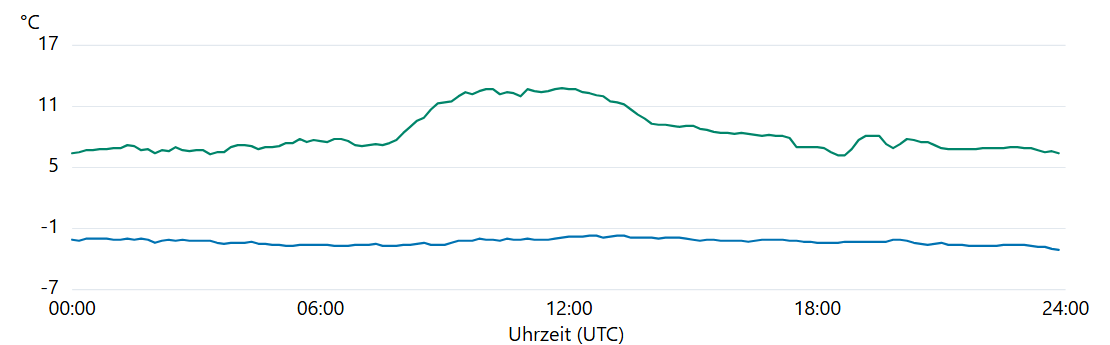
\includegraphics[width=\linewidth,height=0.38\textheight,keepaspectratio]{Abbildungen/anwendungsfall_dezember.png}
  \par\smallskip
  {\small\begin{tabular}{lrr}
  Station & Vorhandene Werte & Temperaturmittel \\
  \hline \textcolor[HTML]{0072b2}{Wittenberg} & 144/144 & $-2{,}30$\,°C \\
  \textcolor[HTML]{00856a}{Brocken} & 144/144 & 8,42\,°C \\
  \end{tabular}\par}
  \caption{Temperaturdiagramm nach Auswahl des 28. Dezember in der
  Differenzübersicht. Brocken ist an diesem Tag im Mittel 10,72\,°C
  wärmer als Wittenberg. Beide Reihen besitzen vollständige Abdeckung.}
  \label{fig:case-december}
\end{figure}

Die unabhängige vollständige Jahresauswertung enthält 354 verwendbare
Vergleichstage: An 331 ist Wittenberg im Mittel wärmer, an 23 Brocken.
Zwölf Tage bleiben unvollständig und werden nicht als Nullunterschiede
gewertet. Der 28. Dezember besitzt den kleinsten Wert von Wittenberg minus
Brocken ($-10{,}72$\,°C), der 27. September den größten
(10,20\,°C). Diese Rangfolge stammt aus der rechnerischen Auswertung;
die Farbklassen allein unterscheiden keine Rangfolge innerhalb einer Klasse.

\begin{figure}[htbp]
  \centering
  % Generiert aus stationsdifferenzen.csv; A=Wittenberg, B=Brocken.
\begingroup\setlength{\unitlength}{1pt}
\begin{picture}(420,266)
\put(0,252){\small (a) Recursive Pattern}
\put(225,252){\small (b) Kalender: Mo bis So}
\put(0,227){\color[HTML]{d6604d}\rule{7pt}{7pt}}
\put(7,227){\color[HTML]{f4a582}\rule{7pt}{7pt}}
\put(14,227){\color[HTML]{d6604d}\rule{7pt}{7pt}}
\put(21,227){\color[HTML]{d6604d}\rule{7pt}{7pt}}
\put(28,227){\color[HTML]{f4a582}\rule{7pt}{7pt}}
\put(35,227){\color[HTML]{fddbc7}\rule{7pt}{7pt}}
\put(42,227){\color[HTML]{d6604d}\rule{7pt}{7pt}}
\put(0,220){\color[HTML]{d6604d}\rule{7pt}{7pt}}
\put(7,220){\color[HTML]{d1e5f0}\rule{7pt}{7pt}}
\put(14,220){\color[HTML]{92c5de}\rule{7pt}{7pt}}
\put(21,220){\color[HTML]{92c5de}\rule{7pt}{7pt}}
\put(28,220){\color[HTML]{f4a582}\rule{7pt}{7pt}}
\put(35,220){\color[HTML]{d6604d}\rule{7pt}{7pt}}
\put(42,220){\color[HTML]{d6604d}\rule{7pt}{7pt}}
\put(0,213){\color[HTML]{d6604d}\rule{7pt}{7pt}}
\put(7,213){\color[HTML]{d6604d}\rule{7pt}{7pt}}
\put(14,213){\color[HTML]{f4a582}\rule{7pt}{7pt}}
\put(21,213){\color[HTML]{f4a582}\rule{7pt}{7pt}}
\put(28,213){\color[HTML]{f4a582}\rule{7pt}{7pt}}
\put(35,213){\color[HTML]{f4a582}\rule{7pt}{7pt}}
\put(42,213){\color[HTML]{f4a582}\rule{7pt}{7pt}}
\put(0,206){\color[HTML]{d6604d}\rule{7pt}{7pt}}
\put(7,206){\color[HTML]{d6604d}\rule{7pt}{7pt}}
\put(14,206){\color[HTML]{d6604d}\rule{7pt}{7pt}}
\put(21,206){\color[HTML]{d6604d}\rule{7pt}{7pt}}
\put(28,206){\color[HTML]{f4a582}\rule{7pt}{7pt}}
\put(35,206){\color[HTML]{d6604d}\rule{7pt}{7pt}}
\put(42,206){\color[HTML]{d1e5f0}\rule{7pt}{7pt}}
\put(0,199){\color[HTML]{92c5de}\rule{7pt}{7pt}}
\put(7,199){\color[HTML]{fddbc7}\rule{7pt}{7pt}}
\put(14,199){\color[HTML]{d6604d}\rule{7pt}{7pt}}
\put(21,199){\color[HTML]{d6604d}\rule{7pt}{7pt}}
\put(28,199){\color[HTML]{d6604d}\rule{7pt}{7pt}}
\put(35,199){\color[HTML]{d6604d}\rule{7pt}{7pt}}
\put(42,199){\color[HTML]{d6604d}\rule{7pt}{7pt}}
\put(0,192){\color[HTML]{d6604d}\rule{7pt}{7pt}}
\put(7,192){\color[HTML]{d6604d}\rule{7pt}{7pt}}
\put(14,192){\color[HTML]{d6604d}\rule{7pt}{7pt}}
\put(21,192){\color[HTML]{f4a582}\rule{7pt}{7pt}}
\put(28,192){\color[HTML]{f4a582}\rule{7pt}{7pt}}
\put(35,192){\color[HTML]{d6604d}\rule{7pt}{7pt}}
\put(42,192){\color[HTML]{f4a582}\rule{7pt}{7pt}}
\put(61,227){\color[HTML]{d6604d}\rule{7pt}{7pt}}
\put(68,227){\color[HTML]{d6604d}\rule{7pt}{7pt}}
\put(75,227){\color[HTML]{d6604d}\rule{7pt}{7pt}}
\put(82,227){\color[HTML]{d6604d}\rule{7pt}{7pt}}
\put(89,227){\color[HTML]{f4a582}\rule{7pt}{7pt}}
\put(96,227){\color[HTML]{d6604d}\rule{7pt}{7pt}}
\put(103,227){\color[HTML]{f4a582}\rule{7pt}{7pt}}
\put(61,220){\color[HTML]{d6604d}\rule{7pt}{7pt}}
\put(68,220){\color[HTML]{d6604d}\rule{7pt}{7pt}}
\put(75,220){\color[HTML]{d6604d}\rule{7pt}{7pt}}
\put(82,220){\color[HTML]{d6604d}\rule{7pt}{7pt}}
\put(89,220){\color[HTML]{d6604d}\rule{7pt}{7pt}}
\put(96,220){\color[HTML]{d6604d}\rule{7pt}{7pt}}
\put(103,220){\color[HTML]{d6604d}\rule{7pt}{7pt}}
\put(61,213){\color[HTML]{d6604d}\rule{7pt}{7pt}}
\put(68,213){\color[HTML]{d6604d}\rule{7pt}{7pt}}
\put(75,213){\color[HTML]{f4a582}\rule{7pt}{7pt}}
\put(82,213){\color[HTML]{f4a582}\rule{7pt}{7pt}}
\put(89,213){\color[HTML]{f4a582}\rule{7pt}{7pt}}
\put(96,213){\color[HTML]{d6604d}\rule{7pt}{7pt}}
\put(103,213){\color[HTML]{f4a582}\rule{7pt}{7pt}}
\put(61,206){\color[HTML]{f4a582}\rule{7pt}{7pt}}
\put(68,206){\color[HTML]{d6604d}\rule{7pt}{7pt}}
\put(75,206){\color[HTML]{d6604d}\rule{7pt}{7pt}}
\put(82,206){\color[HTML]{d6604d}\rule{7pt}{7pt}}
\put(89,206){\color[HTML]{d6604d}\rule{7pt}{7pt}}
\put(96,206){\color[HTML]{d6604d}\rule{7pt}{7pt}}
\put(103,206){\color[HTML]{d6604d}\rule{7pt}{7pt}}
\put(61,199){\color[HTML]{d6604d}\rule{7pt}{7pt}}
\put(68,199){\color[HTML]{d6604d}\rule{7pt}{7pt}}
\put(75,199){\color[HTML]{d6604d}\rule{7pt}{7pt}}
\put(82,199){\color[HTML]{d6604d}\rule{7pt}{7pt}}
\put(89,199){\color[HTML]{d6604d}\rule{7pt}{7pt}}
\put(96,199){\color[HTML]{d6604d}\rule{7pt}{7pt}}
\put(103,199){\color[HTML]{f4a582}\rule{7pt}{7pt}}
\put(61,192){\color[HTML]{fddbc7}\rule{7pt}{7pt}}
\put(68,192){\color[HTML]{fddbc7}\rule{7pt}{7pt}}
\put(75,192){\color[HTML]{f4a582}\rule{7pt}{7pt}}
\put(82,192){\color[HTML]{d6604d}\rule{7pt}{7pt}}
\put(89,192){\color[HTML]{d6604d}\rule{7pt}{7pt}}
\put(96,192){\color[HTML]{d6604d}\rule{7pt}{7pt}}
\put(103,192){\color[HTML]{d6604d}\rule{7pt}{7pt}}
\put(122,227){\color[HTML]{d6604d}\rule{7pt}{7pt}}
\put(129,227){\color[HTML]{d6604d}\rule{7pt}{7pt}}
\put(136,227){\color[HTML]{f4a582}\rule{7pt}{7pt}}
\put(143,227){\color[HTML]{d6604d}\rule{7pt}{7pt}}
\put(150,227){\color[HTML]{d6604d}\rule{7pt}{7pt}}
\put(157,227){\color[HTML]{d6604d}\rule{7pt}{7pt}}
\put(164,227){\color[HTML]{d6604d}\rule{7pt}{7pt}}
\put(122,220){\color[HTML]{d6604d}\rule{7pt}{7pt}}
\put(129,220){\color[HTML]{d6604d}\rule{7pt}{7pt}}
\put(136,220){\color[HTML]{d6604d}\rule{7pt}{7pt}}
\put(143,220){\color[HTML]{d6604d}\rule{7pt}{7pt}}
\put(150,220){\color[HTML]{d6604d}\rule{7pt}{7pt}}
\put(157,220){\color[HTML]{bbbbbb}\rule{7pt}{7pt}}
\put(157,220){\color{black}\rotatebox{45}{\rule{9.899pt}{0.25pt}}}
\put(164,220){\color[HTML]{bbbbbb}\rule{7pt}{7pt}}
\put(164,220){\color{black}\rotatebox{45}{\rule{9.899pt}{0.25pt}}}
\put(122,213){\color[HTML]{bbbbbb}\rule{7pt}{7pt}}
\put(122,213){\color{black}\rotatebox{45}{\rule{9.899pt}{0.25pt}}}
\put(129,213){\color[HTML]{d6604d}\rule{7pt}{7pt}}
\put(136,213){\color[HTML]{d6604d}\rule{7pt}{7pt}}
\put(143,213){\color[HTML]{d6604d}\rule{7pt}{7pt}}
\put(150,213){\color[HTML]{d6604d}\rule{7pt}{7pt}}
\put(157,213){\color[HTML]{d6604d}\rule{7pt}{7pt}}
\put(164,213){\color[HTML]{d6604d}\rule{7pt}{7pt}}
\put(122,206){\color[HTML]{d6604d}\rule{7pt}{7pt}}
\put(129,206){\color[HTML]{d6604d}\rule{7pt}{7pt}}
\put(136,206){\color[HTML]{d6604d}\rule{7pt}{7pt}}
\put(143,206){\color[HTML]{d6604d}\rule{7pt}{7pt}}
\put(150,206){\color[HTML]{d6604d}\rule{7pt}{7pt}}
\put(157,206){\color[HTML]{d6604d}\rule{7pt}{7pt}}
\put(164,206){\color[HTML]{d6604d}\rule{7pt}{7pt}}
\put(122,199){\color[HTML]{d6604d}\rule{7pt}{7pt}}
\put(129,199){\color[HTML]{d6604d}\rule{7pt}{7pt}}
\put(136,199){\color[HTML]{d6604d}\rule{7pt}{7pt}}
\put(143,199){\color[HTML]{d6604d}\rule{7pt}{7pt}}
\put(150,199){\color[HTML]{d6604d}\rule{7pt}{7pt}}
\put(157,199){\color[HTML]{d6604d}\rule{7pt}{7pt}}
\put(164,199){\color[HTML]{d6604d}\rule{7pt}{7pt}}
\put(122,192){\color[HTML]{d6604d}\rule{7pt}{7pt}}
\put(129,192){\color[HTML]{d6604d}\rule{7pt}{7pt}}
\put(136,192){\color[HTML]{d6604d}\rule{7pt}{7pt}}
\put(143,192){\color[HTML]{d6604d}\rule{7pt}{7pt}}
\put(150,192){\color[HTML]{d6604d}\rule{7pt}{7pt}}
\put(157,192){\color[HTML]{d6604d}\rule{7pt}{7pt}}
\put(164,192){\color[HTML]{d6604d}\rule{7pt}{7pt}}
\put(0,162){\color[HTML]{d6604d}\rule{7pt}{7pt}}
\put(7,162){\color[HTML]{d6604d}\rule{7pt}{7pt}}
\put(14,162){\color[HTML]{d6604d}\rule{7pt}{7pt}}
\put(21,162){\color[HTML]{d6604d}\rule{7pt}{7pt}}
\put(28,162){\color[HTML]{d6604d}\rule{7pt}{7pt}}
\put(35,162){\color[HTML]{d6604d}\rule{7pt}{7pt}}
\put(42,162){\color[HTML]{d6604d}\rule{7pt}{7pt}}
\put(0,155){\color[HTML]{d6604d}\rule{7pt}{7pt}}
\put(7,155){\color[HTML]{d6604d}\rule{7pt}{7pt}}
\put(14,155){\color[HTML]{d6604d}\rule{7pt}{7pt}}
\put(21,155){\color[HTML]{b2182b}\rule{7pt}{7pt}}
\put(28,155){\color[HTML]{d6604d}\rule{7pt}{7pt}}
\put(35,155){\color[HTML]{d6604d}\rule{7pt}{7pt}}
\put(42,155){\color[HTML]{d6604d}\rule{7pt}{7pt}}
\put(0,148){\color[HTML]{d6604d}\rule{7pt}{7pt}}
\put(7,148){\color[HTML]{d6604d}\rule{7pt}{7pt}}
\put(14,148){\color[HTML]{d6604d}\rule{7pt}{7pt}}
\put(21,148){\color[HTML]{d6604d}\rule{7pt}{7pt}}
\put(28,148){\color[HTML]{d6604d}\rule{7pt}{7pt}}
\put(35,148){\color[HTML]{d6604d}\rule{7pt}{7pt}}
\put(42,148){\color[HTML]{bbbbbb}\rule{7pt}{7pt}}
\put(42,148){\color{black}\rotatebox{45}{\rule{9.899pt}{0.25pt}}}
\put(0,141){\color[HTML]{bbbbbb}\rule{7pt}{7pt}}
\put(0,141){\color{black}\rotatebox{45}{\rule{9.899pt}{0.25pt}}}
\put(7,141){\color[HTML]{bbbbbb}\rule{7pt}{7pt}}
\put(7,141){\color{black}\rotatebox{45}{\rule{9.899pt}{0.25pt}}}
\put(14,141){\color[HTML]{d6604d}\rule{7pt}{7pt}}
\put(21,141){\color[HTML]{d6604d}\rule{7pt}{7pt}}
\put(28,141){\color[HTML]{d6604d}\rule{7pt}{7pt}}
\put(35,141){\color[HTML]{d6604d}\rule{7pt}{7pt}}
\put(42,141){\color[HTML]{d6604d}\rule{7pt}{7pt}}
\put(0,134){\color[HTML]{bbbbbb}\rule{7pt}{7pt}}
\put(0,134){\color{black}\rotatebox{45}{\rule{9.899pt}{0.25pt}}}
\put(7,134){\color[HTML]{d6604d}\rule{7pt}{7pt}}
\put(14,134){\color[HTML]{d6604d}\rule{7pt}{7pt}}
\put(21,134){\color[HTML]{d6604d}\rule{7pt}{7pt}}
\put(28,134){\color[HTML]{d6604d}\rule{7pt}{7pt}}
\put(35,134){\color[HTML]{d6604d}\rule{7pt}{7pt}}
\put(42,134){\color[HTML]{d6604d}\rule{7pt}{7pt}}
\put(0,127){\color[HTML]{d6604d}\rule{7pt}{7pt}}
\put(7,127){\color[HTML]{d6604d}\rule{7pt}{7pt}}
\put(14,127){\color[HTML]{d6604d}\rule{7pt}{7pt}}
\put(21,127){\color[HTML]{d6604d}\rule{7pt}{7pt}}
\put(28,127){\color[HTML]{d6604d}\rule{7pt}{7pt}}
\put(35,127){\color[HTML]{d6604d}\rule{7pt}{7pt}}
\put(42,127){\color[HTML]{d6604d}\rule{7pt}{7pt}}
\put(61,162){\color[HTML]{d6604d}\rule{7pt}{7pt}}
\put(68,162){\color[HTML]{d6604d}\rule{7pt}{7pt}}
\put(75,162){\color[HTML]{d6604d}\rule{7pt}{7pt}}
\put(82,162){\color[HTML]{d6604d}\rule{7pt}{7pt}}
\put(89,162){\color[HTML]{d6604d}\rule{7pt}{7pt}}
\put(96,162){\color[HTML]{d6604d}\rule{7pt}{7pt}}
\put(103,162){\color[HTML]{d6604d}\rule{7pt}{7pt}}
\put(61,155){\color[HTML]{d6604d}\rule{7pt}{7pt}}
\put(68,155){\color[HTML]{bbbbbb}\rule{7pt}{7pt}}
\put(68,155){\color{black}\rotatebox{45}{\rule{9.899pt}{0.25pt}}}
\put(75,155){\color[HTML]{bbbbbb}\rule{7pt}{7pt}}
\put(75,155){\color{black}\rotatebox{45}{\rule{9.899pt}{0.25pt}}}
\put(82,155){\color[HTML]{d6604d}\rule{7pt}{7pt}}
\put(89,155){\color[HTML]{d6604d}\rule{7pt}{7pt}}
\put(96,155){\color[HTML]{d6604d}\rule{7pt}{7pt}}
\put(103,155){\color[HTML]{d6604d}\rule{7pt}{7pt}}
\put(61,148){\color[HTML]{d6604d}\rule{7pt}{7pt}}
\put(68,148){\color[HTML]{d6604d}\rule{7pt}{7pt}}
\put(75,148){\color[HTML]{d6604d}\rule{7pt}{7pt}}
\put(82,148){\color[HTML]{d6604d}\rule{7pt}{7pt}}
\put(89,148){\color[HTML]{d6604d}\rule{7pt}{7pt}}
\put(96,148){\color[HTML]{d6604d}\rule{7pt}{7pt}}
\put(103,148){\color[HTML]{d6604d}\rule{7pt}{7pt}}
\put(61,141){\color[HTML]{d6604d}\rule{7pt}{7pt}}
\put(68,141){\color[HTML]{d6604d}\rule{7pt}{7pt}}
\put(75,141){\color[HTML]{d6604d}\rule{7pt}{7pt}}
\put(82,141){\color[HTML]{d6604d}\rule{7pt}{7pt}}
\put(89,141){\color[HTML]{d6604d}\rule{7pt}{7pt}}
\put(96,141){\color[HTML]{d6604d}\rule{7pt}{7pt}}
\put(103,141){\color[HTML]{d6604d}\rule{7pt}{7pt}}
\put(61,134){\color[HTML]{d6604d}\rule{7pt}{7pt}}
\put(68,134){\color[HTML]{b2182b}\rule{7pt}{7pt}}
\put(75,134){\color[HTML]{d6604d}\rule{7pt}{7pt}}
\put(82,134){\color[HTML]{d6604d}\rule{7pt}{7pt}}
\put(89,134){\color[HTML]{d6604d}\rule{7pt}{7pt}}
\put(96,134){\color[HTML]{d6604d}\rule{7pt}{7pt}}
\put(103,134){\color[HTML]{d6604d}\rule{7pt}{7pt}}
\put(61,127){\color[HTML]{d6604d}\rule{7pt}{7pt}}
\put(68,127){\color[HTML]{d6604d}\rule{7pt}{7pt}}
\put(75,127){\color[HTML]{d6604d}\rule{7pt}{7pt}}
\put(82,127){\color[HTML]{d6604d}\rule{7pt}{7pt}}
\put(89,127){\color[HTML]{d6604d}\rule{7pt}{7pt}}
\put(96,127){\color[HTML]{d6604d}\rule{7pt}{7pt}}
\put(103,127){\color[HTML]{d6604d}\rule{7pt}{7pt}}
\put(122,162){\color[HTML]{f4a582}\rule{7pt}{7pt}}
\put(129,162){\color[HTML]{f4a582}\rule{7pt}{7pt}}
\put(136,162){\color[HTML]{d6604d}\rule{7pt}{7pt}}
\put(143,162){\color[HTML]{d6604d}\rule{7pt}{7pt}}
\put(150,162){\color[HTML]{d6604d}\rule{7pt}{7pt}}
\put(157,162){\color[HTML]{d6604d}\rule{7pt}{7pt}}
\put(164,162){\color[HTML]{d6604d}\rule{7pt}{7pt}}
\put(122,155){\color[HTML]{d6604d}\rule{7pt}{7pt}}
\put(129,155){\color[HTML]{f4a582}\rule{7pt}{7pt}}
\put(136,155){\color[HTML]{d6604d}\rule{7pt}{7pt}}
\put(143,155){\color[HTML]{d6604d}\rule{7pt}{7pt}}
\put(150,155){\color[HTML]{d6604d}\rule{7pt}{7pt}}
\put(157,155){\color[HTML]{d6604d}\rule{7pt}{7pt}}
\put(164,155){\color[HTML]{d6604d}\rule{7pt}{7pt}}
\put(122,148){\color[HTML]{f4a582}\rule{7pt}{7pt}}
\put(129,148){\color[HTML]{f4a582}\rule{7pt}{7pt}}
\put(136,148){\color[HTML]{f4a582}\rule{7pt}{7pt}}
\put(143,148){\color[HTML]{d6604d}\rule{7pt}{7pt}}
\put(150,148){\color[HTML]{d6604d}\rule{7pt}{7pt}}
\put(157,148){\color[HTML]{d6604d}\rule{7pt}{7pt}}
\put(164,148){\color[HTML]{d6604d}\rule{7pt}{7pt}}
\put(122,141){\color[HTML]{d6604d}\rule{7pt}{7pt}}
\put(129,141){\color[HTML]{d6604d}\rule{7pt}{7pt}}
\put(136,141){\color[HTML]{d6604d}\rule{7pt}{7pt}}
\put(143,141){\color[HTML]{d6604d}\rule{7pt}{7pt}}
\put(150,141){\color[HTML]{d6604d}\rule{7pt}{7pt}}
\put(157,141){\color[HTML]{d6604d}\rule{7pt}{7pt}}
\put(164,141){\color[HTML]{d6604d}\rule{7pt}{7pt}}
\put(122,134){\color[HTML]{d6604d}\rule{7pt}{7pt}}
\put(129,134){\color[HTML]{d6604d}\rule{7pt}{7pt}}
\put(136,134){\color[HTML]{d6604d}\rule{7pt}{7pt}}
\put(143,134){\color[HTML]{d6604d}\rule{7pt}{7pt}}
\put(150,134){\color[HTML]{d6604d}\rule{7pt}{7pt}}
\put(157,134){\color[HTML]{d6604d}\rule{7pt}{7pt}}
\put(164,134){\color[HTML]{d6604d}\rule{7pt}{7pt}}
\put(122,127){\color[HTML]{f4a582}\rule{7pt}{7pt}}
\put(129,127){\color[HTML]{d6604d}\rule{7pt}{7pt}}
\put(136,127){\color[HTML]{d6604d}\rule{7pt}{7pt}}
\put(143,127){\color[HTML]{d6604d}\rule{7pt}{7pt}}
\put(150,127){\color[HTML]{d6604d}\rule{7pt}{7pt}}
\put(157,127){\color[HTML]{d6604d}\rule{7pt}{7pt}}
\put(164,127){\color[HTML]{d6604d}\rule{7pt}{7pt}}
\put(0,97){\color[HTML]{d6604d}\rule{7pt}{7pt}}
\put(7,97){\color[HTML]{d6604d}\rule{7pt}{7pt}}
\put(14,97){\color[HTML]{d6604d}\rule{7pt}{7pt}}
\put(21,97){\color[HTML]{d6604d}\rule{7pt}{7pt}}
\put(28,97){\color[HTML]{d6604d}\rule{7pt}{7pt}}
\put(35,97){\color[HTML]{d6604d}\rule{7pt}{7pt}}
\put(42,97){\color[HTML]{d6604d}\rule{7pt}{7pt}}
\put(0,90){\color[HTML]{d6604d}\rule{7pt}{7pt}}
\put(7,90){\color[HTML]{d6604d}\rule{7pt}{7pt}}
\put(14,90){\color[HTML]{d6604d}\rule{7pt}{7pt}}
\put(21,90){\color[HTML]{d6604d}\rule{7pt}{7pt}}
\put(28,90){\color[HTML]{d6604d}\rule{7pt}{7pt}}
\put(35,90){\color[HTML]{d6604d}\rule{7pt}{7pt}}
\put(42,90){\color[HTML]{f4a582}\rule{7pt}{7pt}}
\put(0,83){\color[HTML]{f4a582}\rule{7pt}{7pt}}
\put(7,83){\color[HTML]{d6604d}\rule{7pt}{7pt}}
\put(14,83){\color[HTML]{d6604d}\rule{7pt}{7pt}}
\put(21,83){\color[HTML]{d6604d}\rule{7pt}{7pt}}
\put(28,83){\color[HTML]{b2182b}\rule{7pt}{7pt}}
\put(35,83){\color[HTML]{d6604d}\rule{7pt}{7pt}}
\put(42,83){\color[HTML]{d6604d}\rule{7pt}{7pt}}
\put(0,76){\color[HTML]{d6604d}\rule{7pt}{7pt}}
\put(7,76){\color[HTML]{d6604d}\rule{7pt}{7pt}}
\put(14,76){\color[HTML]{d6604d}\rule{7pt}{7pt}}
\put(21,76){\color[HTML]{d6604d}\rule{7pt}{7pt}}
\put(28,76){\color[HTML]{d6604d}\rule{7pt}{7pt}}
\put(35,76){\color[HTML]{d6604d}\rule{7pt}{7pt}}
\put(42,76){\color[HTML]{d6604d}\rule{7pt}{7pt}}
\put(0,69){\color[HTML]{f4a582}\rule{7pt}{7pt}}
\put(7,69){\color[HTML]{d6604d}\rule{7pt}{7pt}}
\put(14,69){\color[HTML]{d6604d}\rule{7pt}{7pt}}
\put(21,69){\color[HTML]{d6604d}\rule{7pt}{7pt}}
\put(28,69){\color[HTML]{d6604d}\rule{7pt}{7pt}}
\put(35,69){\color[HTML]{d6604d}\rule{7pt}{7pt}}
\put(42,69){\color[HTML]{d6604d}\rule{7pt}{7pt}}
\put(0,62){\color[HTML]{d6604d}\rule{7pt}{7pt}}
\put(7,62){\color[HTML]{f4a582}\rule{7pt}{7pt}}
\put(14,62){\color[HTML]{f4a582}\rule{7pt}{7pt}}
\put(21,62){\color[HTML]{d1e5f0}\rule{7pt}{7pt}}
\put(28,62){\color[HTML]{d1e5f0}\rule{7pt}{7pt}}
\put(35,62){\color[HTML]{f4a582}\rule{7pt}{7pt}}
\put(42,62){\color[HTML]{f4a582}\rule{7pt}{7pt}}
\put(61,97){\color[HTML]{d6604d}\rule{7pt}{7pt}}
\put(68,97){\color[HTML]{d6604d}\rule{7pt}{7pt}}
\put(75,97){\color[HTML]{f4a582}\rule{7pt}{7pt}}
\put(82,97){\color[HTML]{f4a582}\rule{7pt}{7pt}}
\put(89,97){\color[HTML]{fddbc7}\rule{7pt}{7pt}}
\put(96,97){\color[HTML]{fddbc7}\rule{7pt}{7pt}}
\put(103,97){\color[HTML]{bbbbbb}\rule{7pt}{7pt}}
\put(103,97){\color{black}\rotatebox{45}{\rule{9.899pt}{0.25pt}}}
\put(61,90){\color[HTML]{bbbbbb}\rule{7pt}{7pt}}
\put(61,90){\color{black}\rotatebox{45}{\rule{9.899pt}{0.25pt}}}
\put(68,90){\color[HTML]{bbbbbb}\rule{7pt}{7pt}}
\put(68,90){\color{black}\rotatebox{45}{\rule{9.899pt}{0.25pt}}}
\put(75,90){\color[HTML]{d6604d}\rule{7pt}{7pt}}
\put(82,90){\color[HTML]{f4a582}\rule{7pt}{7pt}}
\put(89,90){\color[HTML]{f4a582}\rule{7pt}{7pt}}
\put(96,90){\color[HTML]{d6604d}\rule{7pt}{7pt}}
\put(103,90){\color[HTML]{4393c3}\rule{7pt}{7pt}}
\put(61,83){\color[HTML]{92c5de}\rule{7pt}{7pt}}
\put(68,83){\color[HTML]{4393c3}\rule{7pt}{7pt}}
\put(75,83){\color[HTML]{92c5de}\rule{7pt}{7pt}}
\put(82,83){\color[HTML]{92c5de}\rule{7pt}{7pt}}
\put(89,83){\color[HTML]{f4a582}\rule{7pt}{7pt}}
\put(96,83){\color[HTML]{92c5de}\rule{7pt}{7pt}}
\put(103,83){\color[HTML]{4393c3}\rule{7pt}{7pt}}
\put(61,76){\color[HTML]{f4a582}\rule{7pt}{7pt}}
\put(68,76){\color[HTML]{d6604d}\rule{7pt}{7pt}}
\put(75,76){\color[HTML]{f4a582}\rule{7pt}{7pt}}
\put(82,76){\color[HTML]{f4a582}\rule{7pt}{7pt}}
\put(89,76){\color[HTML]{d6604d}\rule{7pt}{7pt}}
\put(96,76){\color[HTML]{d6604d}\rule{7pt}{7pt}}
\put(103,76){\color[HTML]{d6604d}\rule{7pt}{7pt}}
\put(61,69){\color[HTML]{d6604d}\rule{7pt}{7pt}}
\put(68,69){\color[HTML]{d6604d}\rule{7pt}{7pt}}
\put(75,69){\color[HTML]{d6604d}\rule{7pt}{7pt}}
\put(82,69){\color[HTML]{d6604d}\rule{7pt}{7pt}}
\put(89,69){\color[HTML]{d6604d}\rule{7pt}{7pt}}
\put(96,69){\color[HTML]{d6604d}\rule{7pt}{7pt}}
\put(103,69){\color[HTML]{f4a582}\rule{7pt}{7pt}}
\put(61,62){\color[HTML]{d6604d}\rule{7pt}{7pt}}
\put(68,62){\color[HTML]{d6604d}\rule{7pt}{7pt}}
\put(75,62){\color[HTML]{d6604d}\rule{7pt}{7pt}}
\put(82,62){\color[HTML]{d6604d}\rule{7pt}{7pt}}
\put(89,62){\color[HTML]{d6604d}\rule{7pt}{7pt}}
\put(96,62){\color[HTML]{d1e5f0}\rule{7pt}{7pt}}
\put(103,62){\color[HTML]{4393c3}\rule{7pt}{7pt}}
\put(122,97){\color[HTML]{fddbc7}\rule{7pt}{7pt}}
\put(129,97){\color[HTML]{d6604d}\rule{7pt}{7pt}}
\put(136,97){\color[HTML]{d6604d}\rule{7pt}{7pt}}
\put(143,97){\color[HTML]{d6604d}\rule{7pt}{7pt}}
\put(150,97){\color[HTML]{d6604d}\rule{7pt}{7pt}}
\put(157,97){\color[HTML]{d6604d}\rule{7pt}{7pt}}
\put(164,97){\color[HTML]{d6604d}\rule{7pt}{7pt}}
\put(122,90){\color[HTML]{d6604d}\rule{7pt}{7pt}}
\put(129,90){\color[HTML]{f4a582}\rule{7pt}{7pt}}
\put(136,90){\color[HTML]{f4a582}\rule{7pt}{7pt}}
\put(143,90){\color[HTML]{fddbc7}\rule{7pt}{7pt}}
\put(150,90){\color[HTML]{fddbc7}\rule{7pt}{7pt}}
\put(157,90){\color[HTML]{f4a582}\rule{7pt}{7pt}}
\put(164,90){\color[HTML]{d6604d}\rule{7pt}{7pt}}
\put(122,83){\color[HTML]{d6604d}\rule{7pt}{7pt}}
\put(129,83){\color[HTML]{d6604d}\rule{7pt}{7pt}}
\put(136,83){\color[HTML]{d6604d}\rule{7pt}{7pt}}
\put(143,83){\color[HTML]{d6604d}\rule{7pt}{7pt}}
\put(150,83){\color[HTML]{d6604d}\rule{7pt}{7pt}}
\put(157,83){\color[HTML]{d6604d}\rule{7pt}{7pt}}
\put(164,83){\color[HTML]{d6604d}\rule{7pt}{7pt}}
\put(122,76){\color[HTML]{d6604d}\rule{7pt}{7pt}}
\put(129,76){\color[HTML]{f4a582}\rule{7pt}{7pt}}
\put(136,76){\color[HTML]{d1e5f0}\rule{7pt}{7pt}}
\put(143,76){\color[HTML]{92c5de}\rule{7pt}{7pt}}
\put(150,76){\color[HTML]{4393c3}\rule{7pt}{7pt}}
\put(157,76){\color[HTML]{2166ac}\rule{7pt}{7pt}}
\put(157,76){\color{black}\framebox(7,7){}}
\put(164,76){\color[HTML]{4393c3}\rule{7pt}{7pt}}
\put(122,69){\color[HTML]{92c5de}\rule{7pt}{7pt}}
\put(129,69){\color[HTML]{d1e5f0}\rule{7pt}{7pt}}
\put(0,240){\scriptsize Block 1}
\put(61,240){\scriptsize Block 2}
\put(122,240){\scriptsize Block 3}
\put(0,175){\scriptsize Block 4}
\put(61,175){\scriptsize Block 5}
\put(122,175){\scriptsize Block 6}
\put(0,110){\scriptsize Block 7}
\put(61,110){\scriptsize Block 8}
\put(122,110){\scriptsize Block 9}
\put(225,240){\scriptsize Jan.}
\put(225,227){\color[HTML]{d6604d}\rule{7pt}{7pt}}
\put(232,227){\color[HTML]{f4a582}\rule{7pt}{7pt}}
\put(239,227){\color[HTML]{d6604d}\rule{7pt}{7pt}}
\put(246,227){\color[HTML]{d6604d}\rule{7pt}{7pt}}
\put(253,227){\color[HTML]{f4a582}\rule{7pt}{7pt}}
\put(260,227){\color[HTML]{fddbc7}\rule{7pt}{7pt}}
\put(267,227){\color[HTML]{d6604d}\rule{7pt}{7pt}}
\put(225,220){\color[HTML]{d6604d}\rule{7pt}{7pt}}
\put(232,220){\color[HTML]{d1e5f0}\rule{7pt}{7pt}}
\put(239,220){\color[HTML]{92c5de}\rule{7pt}{7pt}}
\put(246,220){\color[HTML]{92c5de}\rule{7pt}{7pt}}
\put(253,220){\color[HTML]{f4a582}\rule{7pt}{7pt}}
\put(260,220){\color[HTML]{d6604d}\rule{7pt}{7pt}}
\put(267,220){\color[HTML]{d6604d}\rule{7pt}{7pt}}
\put(225,213){\color[HTML]{d6604d}\rule{7pt}{7pt}}
\put(232,213){\color[HTML]{d6604d}\rule{7pt}{7pt}}
\put(239,213){\color[HTML]{f4a582}\rule{7pt}{7pt}}
\put(246,213){\color[HTML]{f4a582}\rule{7pt}{7pt}}
\put(253,213){\color[HTML]{f4a582}\rule{7pt}{7pt}}
\put(260,213){\color[HTML]{f4a582}\rule{7pt}{7pt}}
\put(267,213){\color[HTML]{f4a582}\rule{7pt}{7pt}}
\put(225,206){\color[HTML]{d6604d}\rule{7pt}{7pt}}
\put(232,206){\color[HTML]{d6604d}\rule{7pt}{7pt}}
\put(239,206){\color[HTML]{d6604d}\rule{7pt}{7pt}}
\put(246,206){\color[HTML]{d6604d}\rule{7pt}{7pt}}
\put(253,206){\color[HTML]{f4a582}\rule{7pt}{7pt}}
\put(260,206){\color[HTML]{d6604d}\rule{7pt}{7pt}}
\put(267,206){\color[HTML]{d1e5f0}\rule{7pt}{7pt}}
\put(225,199){\color[HTML]{92c5de}\rule{7pt}{7pt}}
\put(232,199){\color[HTML]{fddbc7}\rule{7pt}{7pt}}
\put(239,199){\color[HTML]{d6604d}\rule{7pt}{7pt}}
\put(286,240){\scriptsize Feb.}
\put(307,227){\color[HTML]{d6604d}\rule{7pt}{7pt}}
\put(314,227){\color[HTML]{d6604d}\rule{7pt}{7pt}}
\put(321,227){\color[HTML]{d6604d}\rule{7pt}{7pt}}
\put(328,227){\color[HTML]{d6604d}\rule{7pt}{7pt}}
\put(286,220){\color[HTML]{d6604d}\rule{7pt}{7pt}}
\put(293,220){\color[HTML]{d6604d}\rule{7pt}{7pt}}
\put(300,220){\color[HTML]{d6604d}\rule{7pt}{7pt}}
\put(307,220){\color[HTML]{f4a582}\rule{7pt}{7pt}}
\put(314,220){\color[HTML]{f4a582}\rule{7pt}{7pt}}
\put(321,220){\color[HTML]{d6604d}\rule{7pt}{7pt}}
\put(328,220){\color[HTML]{f4a582}\rule{7pt}{7pt}}
\put(286,213){\color[HTML]{d6604d}\rule{7pt}{7pt}}
\put(293,213){\color[HTML]{d6604d}\rule{7pt}{7pt}}
\put(300,213){\color[HTML]{d6604d}\rule{7pt}{7pt}}
\put(307,213){\color[HTML]{d6604d}\rule{7pt}{7pt}}
\put(314,213){\color[HTML]{f4a582}\rule{7pt}{7pt}}
\put(321,213){\color[HTML]{d6604d}\rule{7pt}{7pt}}
\put(328,213){\color[HTML]{f4a582}\rule{7pt}{7pt}}
\put(286,206){\color[HTML]{d6604d}\rule{7pt}{7pt}}
\put(293,206){\color[HTML]{d6604d}\rule{7pt}{7pt}}
\put(300,206){\color[HTML]{d6604d}\rule{7pt}{7pt}}
\put(307,206){\color[HTML]{d6604d}\rule{7pt}{7pt}}
\put(314,206){\color[HTML]{d6604d}\rule{7pt}{7pt}}
\put(321,206){\color[HTML]{d6604d}\rule{7pt}{7pt}}
\put(328,206){\color[HTML]{d6604d}\rule{7pt}{7pt}}
\put(286,199){\color[HTML]{d6604d}\rule{7pt}{7pt}}
\put(293,199){\color[HTML]{d6604d}\rule{7pt}{7pt}}
\put(300,199){\color[HTML]{f4a582}\rule{7pt}{7pt}}
\put(307,199){\color[HTML]{f4a582}\rule{7pt}{7pt}}
\put(347,240){\scriptsize März}
\put(375,227){\color[HTML]{f4a582}\rule{7pt}{7pt}}
\put(382,227){\color[HTML]{d6604d}\rule{7pt}{7pt}}
\put(389,227){\color[HTML]{f4a582}\rule{7pt}{7pt}}
\put(347,220){\color[HTML]{f4a582}\rule{7pt}{7pt}}
\put(354,220){\color[HTML]{d6604d}\rule{7pt}{7pt}}
\put(361,220){\color[HTML]{d6604d}\rule{7pt}{7pt}}
\put(368,220){\color[HTML]{d6604d}\rule{7pt}{7pt}}
\put(375,220){\color[HTML]{d6604d}\rule{7pt}{7pt}}
\put(382,220){\color[HTML]{d6604d}\rule{7pt}{7pt}}
\put(389,220){\color[HTML]{d6604d}\rule{7pt}{7pt}}
\put(347,213){\color[HTML]{d6604d}\rule{7pt}{7pt}}
\put(354,213){\color[HTML]{d6604d}\rule{7pt}{7pt}}
\put(361,213){\color[HTML]{d6604d}\rule{7pt}{7pt}}
\put(368,213){\color[HTML]{d6604d}\rule{7pt}{7pt}}
\put(375,213){\color[HTML]{d6604d}\rule{7pt}{7pt}}
\put(382,213){\color[HTML]{d6604d}\rule{7pt}{7pt}}
\put(389,213){\color[HTML]{f4a582}\rule{7pt}{7pt}}
\put(347,206){\color[HTML]{fddbc7}\rule{7pt}{7pt}}
\put(354,206){\color[HTML]{fddbc7}\rule{7pt}{7pt}}
\put(361,206){\color[HTML]{f4a582}\rule{7pt}{7pt}}
\put(368,206){\color[HTML]{d6604d}\rule{7pt}{7pt}}
\put(375,206){\color[HTML]{d6604d}\rule{7pt}{7pt}}
\put(382,206){\color[HTML]{d6604d}\rule{7pt}{7pt}}
\put(389,206){\color[HTML]{d6604d}\rule{7pt}{7pt}}
\put(347,199){\color[HTML]{d6604d}\rule{7pt}{7pt}}
\put(354,199){\color[HTML]{d6604d}\rule{7pt}{7pt}}
\put(361,199){\color[HTML]{f4a582}\rule{7pt}{7pt}}
\put(368,199){\color[HTML]{d6604d}\rule{7pt}{7pt}}
\put(375,199){\color[HTML]{d6604d}\rule{7pt}{7pt}}
\put(382,199){\color[HTML]{d6604d}\rule{7pt}{7pt}}
\put(389,199){\color[HTML]{d6604d}\rule{7pt}{7pt}}
\put(225,184){\scriptsize Apr.}
\put(225,171){\color[HTML]{d6604d}\rule{7pt}{7pt}}
\put(232,171){\color[HTML]{d6604d}\rule{7pt}{7pt}}
\put(239,171){\color[HTML]{d6604d}\rule{7pt}{7pt}}
\put(246,171){\color[HTML]{d6604d}\rule{7pt}{7pt}}
\put(253,171){\color[HTML]{d6604d}\rule{7pt}{7pt}}
\put(260,171){\color[HTML]{bbbbbb}\rule{7pt}{7pt}}
\put(260,171){\color{black}\rotatebox{45}{\rule{9.899pt}{0.25pt}}}
\put(267,171){\color[HTML]{bbbbbb}\rule{7pt}{7pt}}
\put(267,171){\color{black}\rotatebox{45}{\rule{9.899pt}{0.25pt}}}
\put(225,164){\color[HTML]{bbbbbb}\rule{7pt}{7pt}}
\put(225,164){\color{black}\rotatebox{45}{\rule{9.899pt}{0.25pt}}}
\put(232,164){\color[HTML]{d6604d}\rule{7pt}{7pt}}
\put(239,164){\color[HTML]{d6604d}\rule{7pt}{7pt}}
\put(246,164){\color[HTML]{d6604d}\rule{7pt}{7pt}}
\put(253,164){\color[HTML]{d6604d}\rule{7pt}{7pt}}
\put(260,164){\color[HTML]{d6604d}\rule{7pt}{7pt}}
\put(267,164){\color[HTML]{d6604d}\rule{7pt}{7pt}}
\put(225,157){\color[HTML]{d6604d}\rule{7pt}{7pt}}
\put(232,157){\color[HTML]{d6604d}\rule{7pt}{7pt}}
\put(239,157){\color[HTML]{d6604d}\rule{7pt}{7pt}}
\put(246,157){\color[HTML]{d6604d}\rule{7pt}{7pt}}
\put(253,157){\color[HTML]{d6604d}\rule{7pt}{7pt}}
\put(260,157){\color[HTML]{d6604d}\rule{7pt}{7pt}}
\put(267,157){\color[HTML]{d6604d}\rule{7pt}{7pt}}
\put(225,150){\color[HTML]{d6604d}\rule{7pt}{7pt}}
\put(232,150){\color[HTML]{d6604d}\rule{7pt}{7pt}}
\put(239,150){\color[HTML]{d6604d}\rule{7pt}{7pt}}
\put(246,150){\color[HTML]{d6604d}\rule{7pt}{7pt}}
\put(253,150){\color[HTML]{d6604d}\rule{7pt}{7pt}}
\put(260,150){\color[HTML]{d6604d}\rule{7pt}{7pt}}
\put(267,150){\color[HTML]{d6604d}\rule{7pt}{7pt}}
\put(225,143){\color[HTML]{d6604d}\rule{7pt}{7pt}}
\put(232,143){\color[HTML]{d6604d}\rule{7pt}{7pt}}
\put(286,184){\scriptsize Mai}
\put(300,171){\color[HTML]{d6604d}\rule{7pt}{7pt}}
\put(307,171){\color[HTML]{d6604d}\rule{7pt}{7pt}}
\put(314,171){\color[HTML]{d6604d}\rule{7pt}{7pt}}
\put(321,171){\color[HTML]{d6604d}\rule{7pt}{7pt}}
\put(328,171){\color[HTML]{d6604d}\rule{7pt}{7pt}}
\put(286,164){\color[HTML]{d6604d}\rule{7pt}{7pt}}
\put(293,164){\color[HTML]{d6604d}\rule{7pt}{7pt}}
\put(300,164){\color[HTML]{d6604d}\rule{7pt}{7pt}}
\put(307,164){\color[HTML]{d6604d}\rule{7pt}{7pt}}
\put(314,164){\color[HTML]{d6604d}\rule{7pt}{7pt}}
\put(321,164){\color[HTML]{d6604d}\rule{7pt}{7pt}}
\put(328,164){\color[HTML]{d6604d}\rule{7pt}{7pt}}
\put(286,157){\color[HTML]{d6604d}\rule{7pt}{7pt}}
\put(293,157){\color[HTML]{d6604d}\rule{7pt}{7pt}}
\put(300,157){\color[HTML]{d6604d}\rule{7pt}{7pt}}
\put(307,157){\color[HTML]{b2182b}\rule{7pt}{7pt}}
\put(314,157){\color[HTML]{d6604d}\rule{7pt}{7pt}}
\put(321,157){\color[HTML]{d6604d}\rule{7pt}{7pt}}
\put(328,157){\color[HTML]{d6604d}\rule{7pt}{7pt}}
\put(286,150){\color[HTML]{d6604d}\rule{7pt}{7pt}}
\put(293,150){\color[HTML]{d6604d}\rule{7pt}{7pt}}
\put(300,150){\color[HTML]{d6604d}\rule{7pt}{7pt}}
\put(307,150){\color[HTML]{d6604d}\rule{7pt}{7pt}}
\put(314,150){\color[HTML]{d6604d}\rule{7pt}{7pt}}
\put(321,150){\color[HTML]{d6604d}\rule{7pt}{7pt}}
\put(328,150){\color[HTML]{bbbbbb}\rule{7pt}{7pt}}
\put(328,150){\color{black}\rotatebox{45}{\rule{9.899pt}{0.25pt}}}
\put(286,143){\color[HTML]{bbbbbb}\rule{7pt}{7pt}}
\put(286,143){\color{black}\rotatebox{45}{\rule{9.899pt}{0.25pt}}}
\put(293,143){\color[HTML]{bbbbbb}\rule{7pt}{7pt}}
\put(293,143){\color{black}\rotatebox{45}{\rule{9.899pt}{0.25pt}}}
\put(300,143){\color[HTML]{d6604d}\rule{7pt}{7pt}}
\put(307,143){\color[HTML]{d6604d}\rule{7pt}{7pt}}
\put(314,143){\color[HTML]{d6604d}\rule{7pt}{7pt}}
\put(347,184){\scriptsize Juni}
\put(382,171){\color[HTML]{d6604d}\rule{7pt}{7pt}}
\put(389,171){\color[HTML]{d6604d}\rule{7pt}{7pt}}
\put(347,164){\color[HTML]{bbbbbb}\rule{7pt}{7pt}}
\put(347,164){\color{black}\rotatebox{45}{\rule{9.899pt}{0.25pt}}}
\put(354,164){\color[HTML]{d6604d}\rule{7pt}{7pt}}
\put(361,164){\color[HTML]{d6604d}\rule{7pt}{7pt}}
\put(368,164){\color[HTML]{d6604d}\rule{7pt}{7pt}}
\put(375,164){\color[HTML]{d6604d}\rule{7pt}{7pt}}
\put(382,164){\color[HTML]{d6604d}\rule{7pt}{7pt}}
\put(389,164){\color[HTML]{d6604d}\rule{7pt}{7pt}}
\put(347,157){\color[HTML]{d6604d}\rule{7pt}{7pt}}
\put(354,157){\color[HTML]{d6604d}\rule{7pt}{7pt}}
\put(361,157){\color[HTML]{d6604d}\rule{7pt}{7pt}}
\put(368,157){\color[HTML]{d6604d}\rule{7pt}{7pt}}
\put(375,157){\color[HTML]{d6604d}\rule{7pt}{7pt}}
\put(382,157){\color[HTML]{d6604d}\rule{7pt}{7pt}}
\put(389,157){\color[HTML]{d6604d}\rule{7pt}{7pt}}
\put(347,150){\color[HTML]{d6604d}\rule{7pt}{7pt}}
\put(354,150){\color[HTML]{d6604d}\rule{7pt}{7pt}}
\put(361,150){\color[HTML]{d6604d}\rule{7pt}{7pt}}
\put(368,150){\color[HTML]{d6604d}\rule{7pt}{7pt}}
\put(375,150){\color[HTML]{d6604d}\rule{7pt}{7pt}}
\put(382,150){\color[HTML]{d6604d}\rule{7pt}{7pt}}
\put(389,150){\color[HTML]{d6604d}\rule{7pt}{7pt}}
\put(347,143){\color[HTML]{d6604d}\rule{7pt}{7pt}}
\put(354,143){\color[HTML]{bbbbbb}\rule{7pt}{7pt}}
\put(354,143){\color{black}\rotatebox{45}{\rule{9.899pt}{0.25pt}}}
\put(361,143){\color[HTML]{bbbbbb}\rule{7pt}{7pt}}
\put(361,143){\color{black}\rotatebox{45}{\rule{9.899pt}{0.25pt}}}
\put(368,143){\color[HTML]{d6604d}\rule{7pt}{7pt}}
\put(375,143){\color[HTML]{d6604d}\rule{7pt}{7pt}}
\put(382,143){\color[HTML]{d6604d}\rule{7pt}{7pt}}
\put(389,143){\color[HTML]{d6604d}\rule{7pt}{7pt}}
\put(225,128){\scriptsize Juli}
\put(225,115){\color[HTML]{d6604d}\rule{7pt}{7pt}}
\put(232,115){\color[HTML]{d6604d}\rule{7pt}{7pt}}
\put(239,115){\color[HTML]{d6604d}\rule{7pt}{7pt}}
\put(246,115){\color[HTML]{d6604d}\rule{7pt}{7pt}}
\put(253,115){\color[HTML]{d6604d}\rule{7pt}{7pt}}
\put(260,115){\color[HTML]{d6604d}\rule{7pt}{7pt}}
\put(267,115){\color[HTML]{d6604d}\rule{7pt}{7pt}}
\put(225,108){\color[HTML]{d6604d}\rule{7pt}{7pt}}
\put(232,108){\color[HTML]{d6604d}\rule{7pt}{7pt}}
\put(239,108){\color[HTML]{d6604d}\rule{7pt}{7pt}}
\put(246,108){\color[HTML]{d6604d}\rule{7pt}{7pt}}
\put(253,108){\color[HTML]{d6604d}\rule{7pt}{7pt}}
\put(260,108){\color[HTML]{d6604d}\rule{7pt}{7pt}}
\put(267,108){\color[HTML]{d6604d}\rule{7pt}{7pt}}
\put(225,101){\color[HTML]{d6604d}\rule{7pt}{7pt}}
\put(232,101){\color[HTML]{b2182b}\rule{7pt}{7pt}}
\put(239,101){\color[HTML]{d6604d}\rule{7pt}{7pt}}
\put(246,101){\color[HTML]{d6604d}\rule{7pt}{7pt}}
\put(253,101){\color[HTML]{d6604d}\rule{7pt}{7pt}}
\put(260,101){\color[HTML]{d6604d}\rule{7pt}{7pt}}
\put(267,101){\color[HTML]{d6604d}\rule{7pt}{7pt}}
\put(225,94){\color[HTML]{d6604d}\rule{7pt}{7pt}}
\put(232,94){\color[HTML]{d6604d}\rule{7pt}{7pt}}
\put(239,94){\color[HTML]{d6604d}\rule{7pt}{7pt}}
\put(246,94){\color[HTML]{d6604d}\rule{7pt}{7pt}}
\put(253,94){\color[HTML]{d6604d}\rule{7pt}{7pt}}
\put(260,94){\color[HTML]{d6604d}\rule{7pt}{7pt}}
\put(267,94){\color[HTML]{d6604d}\rule{7pt}{7pt}}
\put(225,87){\color[HTML]{f4a582}\rule{7pt}{7pt}}
\put(232,87){\color[HTML]{f4a582}\rule{7pt}{7pt}}
\put(239,87){\color[HTML]{d6604d}\rule{7pt}{7pt}}
\put(286,128){\scriptsize Aug.}
\put(307,115){\color[HTML]{d6604d}\rule{7pt}{7pt}}
\put(314,115){\color[HTML]{d6604d}\rule{7pt}{7pt}}
\put(321,115){\color[HTML]{d6604d}\rule{7pt}{7pt}}
\put(328,115){\color[HTML]{d6604d}\rule{7pt}{7pt}}
\put(286,108){\color[HTML]{d6604d}\rule{7pt}{7pt}}
\put(293,108){\color[HTML]{f4a582}\rule{7pt}{7pt}}
\put(300,108){\color[HTML]{d6604d}\rule{7pt}{7pt}}
\put(307,108){\color[HTML]{d6604d}\rule{7pt}{7pt}}
\put(314,108){\color[HTML]{d6604d}\rule{7pt}{7pt}}
\put(321,108){\color[HTML]{d6604d}\rule{7pt}{7pt}}
\put(328,108){\color[HTML]{d6604d}\rule{7pt}{7pt}}
\put(286,101){\color[HTML]{f4a582}\rule{7pt}{7pt}}
\put(293,101){\color[HTML]{f4a582}\rule{7pt}{7pt}}
\put(300,101){\color[HTML]{f4a582}\rule{7pt}{7pt}}
\put(307,101){\color[HTML]{d6604d}\rule{7pt}{7pt}}
\put(314,101){\color[HTML]{d6604d}\rule{7pt}{7pt}}
\put(321,101){\color[HTML]{d6604d}\rule{7pt}{7pt}}
\put(328,101){\color[HTML]{d6604d}\rule{7pt}{7pt}}
\put(286,94){\color[HTML]{d6604d}\rule{7pt}{7pt}}
\put(293,94){\color[HTML]{d6604d}\rule{7pt}{7pt}}
\put(300,94){\color[HTML]{d6604d}\rule{7pt}{7pt}}
\put(307,94){\color[HTML]{d6604d}\rule{7pt}{7pt}}
\put(314,94){\color[HTML]{d6604d}\rule{7pt}{7pt}}
\put(321,94){\color[HTML]{d6604d}\rule{7pt}{7pt}}
\put(328,94){\color[HTML]{d6604d}\rule{7pt}{7pt}}
\put(286,87){\color[HTML]{d6604d}\rule{7pt}{7pt}}
\put(293,87){\color[HTML]{d6604d}\rule{7pt}{7pt}}
\put(300,87){\color[HTML]{d6604d}\rule{7pt}{7pt}}
\put(307,87){\color[HTML]{d6604d}\rule{7pt}{7pt}}
\put(314,87){\color[HTML]{d6604d}\rule{7pt}{7pt}}
\put(321,87){\color[HTML]{d6604d}\rule{7pt}{7pt}}
\put(347,128){\scriptsize Sep.}
\put(389,115){\color[HTML]{d6604d}\rule{7pt}{7pt}}
\put(347,108){\color[HTML]{f4a582}\rule{7pt}{7pt}}
\put(354,108){\color[HTML]{d6604d}\rule{7pt}{7pt}}
\put(361,108){\color[HTML]{d6604d}\rule{7pt}{7pt}}
\put(368,108){\color[HTML]{d6604d}\rule{7pt}{7pt}}
\put(375,108){\color[HTML]{d6604d}\rule{7pt}{7pt}}
\put(382,108){\color[HTML]{d6604d}\rule{7pt}{7pt}}
\put(389,108){\color[HTML]{d6604d}\rule{7pt}{7pt}}
\put(347,101){\color[HTML]{d6604d}\rule{7pt}{7pt}}
\put(354,101){\color[HTML]{d6604d}\rule{7pt}{7pt}}
\put(361,101){\color[HTML]{d6604d}\rule{7pt}{7pt}}
\put(368,101){\color[HTML]{d6604d}\rule{7pt}{7pt}}
\put(375,101){\color[HTML]{d6604d}\rule{7pt}{7pt}}
\put(382,101){\color[HTML]{d6604d}\rule{7pt}{7pt}}
\put(389,101){\color[HTML]{d6604d}\rule{7pt}{7pt}}
\put(347,94){\color[HTML]{d6604d}\rule{7pt}{7pt}}
\put(354,94){\color[HTML]{d6604d}\rule{7pt}{7pt}}
\put(361,94){\color[HTML]{d6604d}\rule{7pt}{7pt}}
\put(368,94){\color[HTML]{d6604d}\rule{7pt}{7pt}}
\put(375,94){\color[HTML]{d6604d}\rule{7pt}{7pt}}
\put(382,94){\color[HTML]{d6604d}\rule{7pt}{7pt}}
\put(389,94){\color[HTML]{f4a582}\rule{7pt}{7pt}}
\put(347,87){\color[HTML]{f4a582}\rule{7pt}{7pt}}
\put(354,87){\color[HTML]{d6604d}\rule{7pt}{7pt}}
\put(361,87){\color[HTML]{d6604d}\rule{7pt}{7pt}}
\put(368,87){\color[HTML]{d6604d}\rule{7pt}{7pt}}
\put(375,87){\color[HTML]{b2182b}\rule{7pt}{7pt}}
\put(382,87){\color[HTML]{d6604d}\rule{7pt}{7pt}}
\put(389,87){\color[HTML]{d6604d}\rule{7pt}{7pt}}
\put(347,80){\color[HTML]{d6604d}\rule{7pt}{7pt}}
\put(225,72){\scriptsize Okt.}
\put(232,59){\color[HTML]{d6604d}\rule{7pt}{7pt}}
\put(239,59){\color[HTML]{d6604d}\rule{7pt}{7pt}}
\put(246,59){\color[HTML]{d6604d}\rule{7pt}{7pt}}
\put(253,59){\color[HTML]{d6604d}\rule{7pt}{7pt}}
\put(260,59){\color[HTML]{d6604d}\rule{7pt}{7pt}}
\put(267,59){\color[HTML]{d6604d}\rule{7pt}{7pt}}
\put(225,52){\color[HTML]{f4a582}\rule{7pt}{7pt}}
\put(232,52){\color[HTML]{d6604d}\rule{7pt}{7pt}}
\put(239,52){\color[HTML]{d6604d}\rule{7pt}{7pt}}
\put(246,52){\color[HTML]{d6604d}\rule{7pt}{7pt}}
\put(253,52){\color[HTML]{d6604d}\rule{7pt}{7pt}}
\put(260,52){\color[HTML]{d6604d}\rule{7pt}{7pt}}
\put(267,52){\color[HTML]{d6604d}\rule{7pt}{7pt}}
\put(225,45){\color[HTML]{d6604d}\rule{7pt}{7pt}}
\put(232,45){\color[HTML]{f4a582}\rule{7pt}{7pt}}
\put(239,45){\color[HTML]{f4a582}\rule{7pt}{7pt}}
\put(246,45){\color[HTML]{d1e5f0}\rule{7pt}{7pt}}
\put(253,45){\color[HTML]{d1e5f0}\rule{7pt}{7pt}}
\put(260,45){\color[HTML]{f4a582}\rule{7pt}{7pt}}
\put(267,45){\color[HTML]{f4a582}\rule{7pt}{7pt}}
\put(225,38){\color[HTML]{d6604d}\rule{7pt}{7pt}}
\put(232,38){\color[HTML]{d6604d}\rule{7pt}{7pt}}
\put(239,38){\color[HTML]{f4a582}\rule{7pt}{7pt}}
\put(246,38){\color[HTML]{f4a582}\rule{7pt}{7pt}}
\put(253,38){\color[HTML]{fddbc7}\rule{7pt}{7pt}}
\put(260,38){\color[HTML]{fddbc7}\rule{7pt}{7pt}}
\put(267,38){\color[HTML]{bbbbbb}\rule{7pt}{7pt}}
\put(267,38){\color{black}\rotatebox{45}{\rule{9.899pt}{0.25pt}}}
\put(225,31){\color[HTML]{bbbbbb}\rule{7pt}{7pt}}
\put(225,31){\color{black}\rotatebox{45}{\rule{9.899pt}{0.25pt}}}
\put(232,31){\color[HTML]{bbbbbb}\rule{7pt}{7pt}}
\put(232,31){\color{black}\rotatebox{45}{\rule{9.899pt}{0.25pt}}}
\put(239,31){\color[HTML]{d6604d}\rule{7pt}{7pt}}
\put(246,31){\color[HTML]{f4a582}\rule{7pt}{7pt}}
\put(286,72){\scriptsize Nov.}
\put(314,59){\color[HTML]{f4a582}\rule{7pt}{7pt}}
\put(321,59){\color[HTML]{d6604d}\rule{7pt}{7pt}}
\put(328,59){\color[HTML]{4393c3}\rule{7pt}{7pt}}
\put(286,52){\color[HTML]{92c5de}\rule{7pt}{7pt}}
\put(293,52){\color[HTML]{4393c3}\rule{7pt}{7pt}}
\put(300,52){\color[HTML]{92c5de}\rule{7pt}{7pt}}
\put(307,52){\color[HTML]{92c5de}\rule{7pt}{7pt}}
\put(314,52){\color[HTML]{f4a582}\rule{7pt}{7pt}}
\put(321,52){\color[HTML]{92c5de}\rule{7pt}{7pt}}
\put(328,52){\color[HTML]{4393c3}\rule{7pt}{7pt}}
\put(286,45){\color[HTML]{f4a582}\rule{7pt}{7pt}}
\put(293,45){\color[HTML]{d6604d}\rule{7pt}{7pt}}
\put(300,45){\color[HTML]{f4a582}\rule{7pt}{7pt}}
\put(307,45){\color[HTML]{f4a582}\rule{7pt}{7pt}}
\put(314,45){\color[HTML]{d6604d}\rule{7pt}{7pt}}
\put(321,45){\color[HTML]{d6604d}\rule{7pt}{7pt}}
\put(328,45){\color[HTML]{d6604d}\rule{7pt}{7pt}}
\put(286,38){\color[HTML]{d6604d}\rule{7pt}{7pt}}
\put(293,38){\color[HTML]{d6604d}\rule{7pt}{7pt}}
\put(300,38){\color[HTML]{d6604d}\rule{7pt}{7pt}}
\put(307,38){\color[HTML]{d6604d}\rule{7pt}{7pt}}
\put(314,38){\color[HTML]{d6604d}\rule{7pt}{7pt}}
\put(321,38){\color[HTML]{d6604d}\rule{7pt}{7pt}}
\put(328,38){\color[HTML]{f4a582}\rule{7pt}{7pt}}
\put(286,31){\color[HTML]{d6604d}\rule{7pt}{7pt}}
\put(293,31){\color[HTML]{d6604d}\rule{7pt}{7pt}}
\put(300,31){\color[HTML]{d6604d}\rule{7pt}{7pt}}
\put(307,31){\color[HTML]{d6604d}\rule{7pt}{7pt}}
\put(314,31){\color[HTML]{d6604d}\rule{7pt}{7pt}}
\put(321,31){\color[HTML]{d1e5f0}\rule{7pt}{7pt}}
\put(347,72){\scriptsize Dez.}
\put(389,59){\color[HTML]{4393c3}\rule{7pt}{7pt}}
\put(347,52){\color[HTML]{fddbc7}\rule{7pt}{7pt}}
\put(354,52){\color[HTML]{d6604d}\rule{7pt}{7pt}}
\put(361,52){\color[HTML]{d6604d}\rule{7pt}{7pt}}
\put(368,52){\color[HTML]{d6604d}\rule{7pt}{7pt}}
\put(375,52){\color[HTML]{d6604d}\rule{7pt}{7pt}}
\put(382,52){\color[HTML]{d6604d}\rule{7pt}{7pt}}
\put(389,52){\color[HTML]{d6604d}\rule{7pt}{7pt}}
\put(347,45){\color[HTML]{d6604d}\rule{7pt}{7pt}}
\put(354,45){\color[HTML]{f4a582}\rule{7pt}{7pt}}
\put(361,45){\color[HTML]{f4a582}\rule{7pt}{7pt}}
\put(368,45){\color[HTML]{fddbc7}\rule{7pt}{7pt}}
\put(375,45){\color[HTML]{fddbc7}\rule{7pt}{7pt}}
\put(382,45){\color[HTML]{f4a582}\rule{7pt}{7pt}}
\put(389,45){\color[HTML]{d6604d}\rule{7pt}{7pt}}
\put(347,38){\color[HTML]{d6604d}\rule{7pt}{7pt}}
\put(354,38){\color[HTML]{d6604d}\rule{7pt}{7pt}}
\put(361,38){\color[HTML]{d6604d}\rule{7pt}{7pt}}
\put(368,38){\color[HTML]{d6604d}\rule{7pt}{7pt}}
\put(375,38){\color[HTML]{d6604d}\rule{7pt}{7pt}}
\put(382,38){\color[HTML]{d6604d}\rule{7pt}{7pt}}
\put(389,38){\color[HTML]{d6604d}\rule{7pt}{7pt}}
\put(347,31){\color[HTML]{d6604d}\rule{7pt}{7pt}}
\put(354,31){\color[HTML]{f4a582}\rule{7pt}{7pt}}
\put(361,31){\color[HTML]{d1e5f0}\rule{7pt}{7pt}}
\put(368,31){\color[HTML]{92c5de}\rule{7pt}{7pt}}
\put(375,31){\color[HTML]{4393c3}\rule{7pt}{7pt}}
\put(382,31){\color[HTML]{2166ac}\rule{7pt}{7pt}}
\put(382,31){\color{black}\framebox(7,7){}}
\put(389,31){\color[HTML]{4393c3}\rule{7pt}{7pt}}
\put(347,24){\color[HTML]{92c5de}\rule{7pt}{7pt}}
\put(354,24){\color[HTML]{d1e5f0}\rule{7pt}{7pt}}
\put(0,12){\footnotesize Rahmen: 28. Dezember. Grau mit Diagonale: unvollständig.}
\put(0,0){\footnotesize Weißraum: kein Datum. Gleiche Zellgröße und Farbgrenzen in beiden Ansichten.}
\end{picture}\endgroup

  \caption{Entwurfsvergleich für dieselbe Frage und dieselben 366 Tage:
  Wittenberg minus Brocken, mit identischen Farbgrenzen wie in
  Abbildung~\ref{fig:difference}. Beide Anordnungen zeigen 354 gültige
  und zwölf unvollständige Vergleichstage. Die Kalenderansicht ist eine
  Vergleichsabbildung für den Bericht, keine zusätzliche Anwendungsansicht.}
  \label{fig:calendar-comparison}
\end{figure}
Die beiden Anordnungen in Abbildung~\ref{fig:calendar-comparison} machen
die Umkehr Ende Dezember durch dieselbe blaue Farbe sichtbar. Für die
Frage nach einem bestimmten Monat ist der Kalender direkter: Seine
Monatsüberschriften und Wochentagsspalten entsprechen vertrauten
Datumsbezügen. Recursive Pattern benötigt dagegen die erläuterte
42-Tage-Leserichtung und den Datumszugriff. Bei gleicher Zellgröße
nutzt es in diesem Entwurf drei Blockzeilen statt vier Monatszeilen;
das schafft Platz für mehrere gleich angeordnete Stationspanels.
Andere Kalenderlayouts können diesen Flächenunterschied verändern.
Die gewählte Technik verbindet den Vorlesungsbezug mit einer festen,
kompakten Jahreszuordnung; der Kalender bleibt eine ernsthafte Alternative.

Für Wetterinteressierte führt die Auswahl eines blauen Tages vom
ungewöhnlichen Stationsverhältnis zu den überprüfbaren Tageskurven.
Eine nach Differenz gefilterte Tabelle findet negative Tage ebenfalls
direkt und liefert exakte Zahlen; die Jahresansicht ergänzt deren
chronologische Umgebung. Für genaue Nulldurchgänge wäre eine
Differenzlinie geeigneter. Die Farbklassen ersetzen diese Aufgaben nicht.
Eine meteorologische Erklärung der beobachteten Umkehr wurde nicht
untersucht; Stationshöhen allein belegen ihre Ursache nicht.

\section{Verwandte Arbeiten}
\subsection{Wetter- und Luftverschmutzungsanalyse in Hongkong}
Qu et al. verbinden Polaransichten mit eingebetteten Pixelbalken,
erweiterte parallele Koordinaten und einen Korrelationsgraphen zur Analyse
von Wetter- und Luftverschmutzungsdaten. Die Aufgaben umfassen
Stationsvergleich, Attributbeziehungen und zeitliche Entwicklung.
Windgeschwindigkeit und Windrichtung bestimmen wichtige Auswahlgesten;
der Korrelationsgraph unterstützt die Achsenanordnung. Abschnitt~5
demonstriert die Verwendung anhand von Fallbeispielen
\autocite[Abschnitte~3--5]{qu2007pollution}.

Gemeinsam ist der Wechsel zwischen Überblick und Untersuchung gefilterter
Stationsdaten. Unsere Profilfilter und Tageswahl koordinieren dafür
Jahres- und Temperaturansichten. Der Unterschied liegt in Aufgabe und
Datenumfang: Vier skalare Wettergrößen eines Jahres unterstützen einen
Vergleich für Wetterinteressierte, während die veröffentlichte Anwendung
die fachliche Untersuchung von Schadstoffbeziehungen verfolgt. Ohne
Windrichtungs- und Schadstoffdaten würde die Übernahme ihrer speziellen
Polar- und Korrelationsansichten unsere festgelegten Fragen nicht lösen.
Qu et al. unterstützen die Achsenanordnung mit einem Korrelationsgraphen.
Für unsere feste Schnittmengenfrage werden Wind und Niederschlag dagegen
gezielt nebeneinander angeordnet; ein Korrelationsgraph wäre dafür ein
zusätzlicher Analyseschritt ohne erforderlichen Nutzen.
Wir verwenden daher vier gerade, fest angeordnete Profilachsen und einen
Temperaturdifferenzüberblick. Der eigene Beitrag liegt in geprüfter
Tageszuordnung, sichtbarer gemeinsamer Abdeckung und den dokumentierten
Bedienabläufen. Wie gut unsere Oberfläche bedienbar ist, lässt sich aus den Fallbeispielen
von Qu et al. allerdings nicht ableiten.

\subsection{Meteorologische Zeitreihen mit Visplore}
Vuckovic und Schmidt untersuchen mit Visplore die Qualität synthetischer
typischer Wetterjahre gegenüber beobachteten meteorologischen Zeitreihen.
Verbundene Analyseansichten unterstützen Qualitätsprüfung, zeitliche
Filterung und Untersuchung verschiedener Granularitäten. Fehlstellen,
Zeitkurven und Verteilungen erhalten unterschiedliche Darstellungen.
Die Autoren beschreiben auch Grenzen der Datenvorbereitung und
betonen die beschränkte Übertragbarkeit der Untersuchung eines Systems
\autocite[Abschnitte~2--4 und~6]{vuckovic2020meteorological}.

Abschnitt~3.2 verbindet Vollständigkeitsprüfung, deskriptive Kennzahlen
und zeitliches Drill-down in einem Qualitätscockpit. Dieser konkrete
Zusammenhang begründet, Messabdeckung neben Tageskennzahlen anzuzeigen:
Ein fehlender Niederschlagswert darf den Wind-/0-mm-Filter nicht erfüllen.
Für unser Projekt ist besonders die Verbindung von Messabdeckung und
zeitlichem Vergleich relevant. Unsere Jahreszellen und Tagesdetails
unterscheiden unvollständige Daten von echten Nullwerten, während die
Zeitraumwahl zwischen Rohwerten und Tagesmitteln wechselt. Der Zweck ist
jedoch ein räumlicher Vergleich beobachteter Stationen von 2024, keine
Validierung eines synthetischen Wetterjahres. Datenabruf und Aggregation
erfolgen unmittelbar in Elm über die Uni-Schnittstelle. Allgemeine
Datenaufbereitung, automatische Mustersuche oder ein umfassender
Qualitätsmonitor sind nicht Teil unseres Systems. Die explizite gemeinsame
Temperaturabdeckung begrenzt hier eine konkrete Vergleichskennzahl.
Die Sieben-Tage-Grenze folgt unserem Entwurf; sie wird nicht aus der
Visplore-Untersuchung als optimale Einstellung abgeleitet.

\subsection{Einordnung der eigenen Anwendung}
Die Übertragung lässt sich auf drei Entwurfsentscheidungen verdichten
(Tabelle~\ref{tab:related-transfer}). Qu et al. begründen den Bezug von
Attributauswahl und koordinierter Detailuntersuchung; Vuckovic und Schmidt
verdeutlichen, warum zeitliche Vergleiche ihre Datenqualität mitführen
müssen \autocite{qu2007pollution,vuckovic2020meteorological}. Unsere
Anwendung verbindet beides für einen begrenzten Stationsvergleich.

\begin{table}[htbp]
  \centering\small
  \begin{tabular}{>{\raggedright\arraybackslash}p{0.27\linewidth}>{\raggedright\arraybackslash}p{0.32\linewidth}>{\raggedright\arraybackslash}p{0.31\linewidth}}
    Bezug & Publizierter Schwerpunkt & Übertragung im Projekt \\
    \hline
    Qu et al.: Attributbeziehungen & Schadstoffe, Windrichtung und anpassbare Achsenanordnung & Vier skalare Wettergrößen; feste benachbarte Wind-/Regenachsen für die Schnittmengenfrage \\
    Vuckovic/Schmidt: Qualität und Zeit & Synthetische Wetterjahre gegenüber beobachteten Reihen; Qualitätscockpit & Beobachtete Stationsdaten; Messabdeckung neben Kennzahlen und offenen Linienlücken \\
    Beide: abgestimmte Untersuchung & Filterung und Zugriff auf zugehörige Details & Profilintervalle, Jahreszellen und Tagesdetails teilen Auswahl und Datum \\
  \end{tabular}
  \caption{Aufgabenbezogene Übertragung aus zwei wissenschaftlichen Anwendungen.}
  \label{tab:related-transfer}
\end{table}

Die Einschränkung auf ein Jahr und vier Stationen ersetzt weder deren
fachliche Funktionen noch die Bewertung ihrer Systeme. Technische
Browserprüfungen belegen hier Berechnungen und Zustandsübergänge; ein
Leistungsvergleich mit den publizierten Anwendungen wurde nicht durchgeführt.

\section{Zusammenfassung und Ausblick}
Die Elm-Anwendung ermöglicht den Vergleich vier deutscher DWD-Stationen
im Jahr 2024 mit drei interaktiv verbundenen Techniken. Recursive Pattern
unterstützt die Jahresorientierung, parallele Koordinaten die Untersuchung
vollständiger Vier-Größen-Profile und Linien die zeitlichen Temperaturdetails.
Tages-, Zeitraum- und Wertebereichsauswahl verbinden diese Teilaufgaben.
Für Wetterinteressierte entsteht der Nutzen daraus, auffällige Tage
auszuwählen und ihre Verläufe und Kennzahlen unmittelbar im gleichen
Stationskontext zu prüfen. Der Differenzmodus benennt die Richtung
A minus B und macht die gemeinsame Temperaturabdeckung sichtbar.

Die Anwendungsfälle zeigen den Nutzen der Verbindung: Ein Monatsvergleich
lässt sich auf eine Woche mit detaillierten Verläufen eingrenzen, eine
gemeinsame Bedingung für Wind und Niederschlag auf vollständigen Tagesprofilen
prüfen und ein Vorzeichenwechsel aus dem Jahresraster unmittelbar im
Tagesverlauf nachvollziehen. Messabdeckung und genaue Kennzahlen bleiben
dabei zugänglich. Die Datenaufbereitung trennt Momentanwerte,
Intervallmittel und Intervallsummen; fehlende Werte werden nicht zu
Nullwerten oder vollständigen Tageskennzahlen. Die unabhängigen Abgleiche
bestätigen die Berechnungen. Die Ergebnisse beschreiben die ausgewählten
Stationen und belegen keine meteorologische Ursache.

Grenzen bestehen in der nicht repräsentativen Stationsauswahl, einem
einzelnen Jahr, nominaler Niederschlagszeitzuordnung, festen Skalen,
Profilüberlagerung und dem Ausschluss unvollständiger Profile.
Die Anwendung kann keine langfristigen Klimatrends belegen. Eine Nutzerstudie zur Verständlichkeit und Bedienung wurde nicht durchgeführt.

Über die statische Gegenüberstellung in Abbildung~\ref{fig:calendar-comparison}
hinaus wäre ein kontrollierter Bedienvergleich mit einer Kalender-Heatmap
sinnvoll. Weitere Erweiterungen wären eine Auswahl weiterer Jahre und Stationen sowie
genauer zugeordnete Standort-/Gerätehistorien. Vor einer Erweiterung
müssten Skalen, Aggregationsregeln und Abrufstrategie erneut geprüft
werden. Vorrangig wäre die Prüfung der Leserichtung und Auswahlzustände mit
der Zielgruppe, bevor weitere Daten die Darstellungsdichte erhöhen.
Dabei könnte untersucht werden, ob
Leserichtung, Differenzvorzeichen und Auflösungswechsel verstanden werden.
Damit ließen sich die bisher begründeten Gestaltungsentscheidungen
über die technischen Tests hinaus bewerten.

\section*{Anhang: Git-Repository}
\url{https://gitlab.informatik.uni-halle.de/amhxr/informationsvisualisierung}

\section*{Anhang: Vorgehen bei der KI-gestützten Entwicklung}
\phantomsection\label{app:ai-workflow}
Die Zusammenarbeit mit Codex umfasste die folgenden Schritte. Dabei
bauten spätere Aufträge auf den bisherigen Entscheidungen und Dateien auf.

\begin{description}
  \item[Aufgaben und Entwurf.]
  Festgelegt wurden Wetter als Thema, vier Stationen, das Jahr 2024 und
  Fragen zum zeitlichen Temperaturvergleich, zu gemeinsamen
  Wetterbedingungen und zur Umkehr von Stationsunterschieden.
  Die Auswahl der Techniken erfolgte anhand dieser Aufgaben und der
  geforderten Visualisierungsbereiche.
  \item[Kontext.]
  Grundlage waren Projektbeschreibung und Berichtsvorlage,
  Vorlesungs- und Übungsunterlagen, Angaben zur HTTP-Schnittstelle und
  zu den Messfeldern sowie verlinkte Implementierungs- und
  Methodenerläuterungen. Das Übungsbeispiel zur rekursiven Anordnung
  konkretisierte die Positionserzeugung. Die Kolleginnenarbeit lieferte
  Orientierung zum Umfang einer Ausarbeitung.
  \item[Schrittweise Erstellung.]
  Codex erstellte zunächst Anmeldung, Datenabruf und Temperaturdarstellung.
  Es folgten Jahresaggregation und Recursive Pattern, Wind und
  Niederschlag mit parallelen Koordinaten sowie Differenzmodus und
  Mehrtagesansicht. Auch Prüfskripte, wissenschaftliche Einordnung und
  Berichtspassagen wurden mit KI-Unterstützung erstellt.
  \item[Bewertung und Anpassung.]
  Die Zwischenergebnisse wurden durchgesehen und mit den Aufgaben
  abgeglichen. Änderungswünsche wurden als weitere Arbeitsaufträge
  formuliert. Größere Überarbeitungen erfolgten durch Codex; kleinere
  manuelle Eingriffe betrafen Layout und Beschriftungspositionen. Diese
  kleinen Änderungen wurden nicht einzeln protokolliert.
  \item[Technische Nachweise.]
  Compiler, echte HTTP-Abrufe, kontrollierte Fehlerantworten und
  CSV-Abgleiche prüften unter anderem Tagesgrenzen, Aggregation,
  fehlende Werte und Auswahlverknüpfungen. Codex führte diese automatisierten Prüfungen aus.
  \item[Weitere Überarbeitung.]
  Ergänzt wurden Profilsuche, Darstellungsmodi, vergrößerbare Jahrespanels,
  begrenzte Rohwertcaches und die gebündelte Stationsübernahme.
  Datenidentische Kalender- und Streudiagrammvergleiche vertieften die
  Abwägung von Alternativen im Bericht.
\end{description}

\printbibliography
\end{document}
